%%% Local Variables:
%%% mode: latex
%%% TeX-master: t
%%% End:

\documentclass[master]{tongjithesis}
% \documentclass[%
%   master|doctor, % mandatory option
%   xetex|pdftex|dvips|dvipdfm, % optional
%   secret,
%   openany|openright,
%   arialtoc,arialtitle]{tongjithesis}

% 所有其它可能用到的包都统一放到这里了,可以根据自己的实际添加或者删除。
\usepackage{tongjiutils}
\usepackage[top=3.8cm, bottom=3.8cm, left=3.2cm, right=3.2cm]{geometry}

% 你可以在这里修改配置文件中的定义,导言区可以使用中文。
\def\myname{邱君诚}

\begin{document}

% 定义所有的eps文件在 figures 子目录下
\graphicspath{{D:/mthall/}{figures/}}

%%% 封面部分
\frontmatter

%%% Local Variables:
%%% mode: latex
%%% TeX-master: t
%%% End:
\secretlevel{保密} 
\secretyear{2}

\ctitle{电容式离子电流检测电路的离子电流适用工况拓展}

% 按照申请工学学位设计。如有其它需要,请修改相应文字。
\makeatletter
  \iftongji@doctor
    \cdegree{工学博士}
  \else
    \iftongji@master
      \cdegree{工学硕士}
    \fi
  \fi

\makeatother

\cdepartment{汽车学院}

\cmajorfirst{动力工程}

\cmajorsecond{}

\cauthor{邱君诚}

\cstnr{1335034}

\degtype{工学}

\csupervisor{吴志军 教授}

% 如果没有副指导老师或者联合指导老师,把各自{}中内容留空即可。

\cassosupervisor{}

\ccosupervisor{}

% 日期自动生成,如果你要自己写就改这个cdate
%\cdate{\CJKdigits{\the\year}年\CJKnumber{\the\month}月}
\makeatletter
  \iftongji@doctor
    \edegree{Doctor of Philosophy}
  \else
    \iftongji@master
      \edegree{Master of Science}
    \fi
  \fi

\makeatother

\cfunds{}

\efunds{}

\etitle{Condition Expand on Ion Current Characteristics Based On Capacitive Detection Circuit}

\edepartment{School of Automotive Study}

\emajorfirst{Power Machinery and Engineering}

\emajorsecond{TONGJILUG}

\edispline{Engineering Science}

\eauthor{Juncheng Qiu}

\esupervisor{Prof. Zhijun Wu}

%\eassosupervisor{Prof. Gang Wan}

% 这个日期也会自动生成,你要改么?
% \edate{May, 2009}

% 定义中英文摘要和关键字
\begin{cabstract}
电容式离子电流检测电路具有性价比高,安装方便的特点。但是由于没有屏蔽点火干扰,随着转速的增加,容易造成点火干扰淹没正常的离子电流信号的弊端。\par
本文通过小波分析的方法很好的将离子电流信号中的点火干扰信号分离出去,获得了理想的离子电流信号。同时比较不同的小波基函数以及小波分析层级,得出了最佳的小波基函数和分解层数。离子电流的火焰后期
信号在理论上近似高斯函数,同时缸内的循环废弃导致的离子电流信号也可以近似成高斯函数,整个检测到的离子电流信号可以用双高斯曲线进行拟合。
采用了拟合算法得到的拟合曲线参数,能够快速地计算出离子电流的各种特征值,能够大大缩小需要的发动机控制系统的计算资源;比较了特征值的估计值和真实值之间的相关性和循环波动率,验证了
双高斯曲线拟合算法估算离子电流特征值的有效性。\par
离子电流的火焰后期开始时刻估计值与结束时刻估计值、最大离子电流升高率估计值与各自对应的特征值有一定的相关性。
离子电流的火焰后期峰值相位估计值、离子电流积分值估计值和最大离子电流升高率相位估计值与各自对应的特征值有明显的相关性。
离子电流积分值和升高率估计值有一定波动,其他特征值的估计值都具有很好的稳定性。
\end{cabstract}

\ckeywords{离子电流, 点火干扰, 小波分析, 高斯曲线}

\begin{eabstract}
Capacitive detection circuit has cost effeciency and is easy to deposit. 
But due to the ignition interfere, the ion current would be submerged by the interfere with the engine speed up.
This is a weak point of this kind of ion current detection circuit.\par
In this paper, real and ideal ion current is extracted
using wavelet analysis method. Different wavelet functions are compared and different wavelet are discussed to dertermine
the best wavelet function and wavelet level. The profile of real ion current in post-frame peroid is similar to that of 
gaussian curve, and the ion current caused by residual waste gas of last cycle also has the similar profile to gaussian
 curve. So the whole ion curren could be simulated by the addition of two gaussian curves and eigen value of ion current
 can be calculated fast by the parameters of two gaussian curves conviniently reducing the computing resource of engine control 
 system. The coefficience of estimated value of each eigen value to each eigen value is validated and fluctuation ratio 
 of each eigen value is calculated to determine the application of double-gaussian method.\par
The time of start and end of post-frame period, the maximum ion rising rate has certain
correspondence to each corresponding eigen value. Ion peak phase, ion integeration and maximum ion
rising rate phase has explicit correspondence to each corresponding eign value.
Despite ion integration and ion rising rate, all the other estimated value have good solidity.
\end{eabstract}

\ekeywords{Ion Current, Ignition Interfere, Wavelet Analysis, Gaussian}

\makecover


% 目录

\tableofcontents

% 符号对照表
\begin{denotation}
\item[GNU] GNU's Not Unix /'gnu:/
\item[GFDL] GNU Free Documentation License
\item[GPL] GNU General Public License
\item[FSF] Free Software Foundation
\item[SMP] �Գƶദ��
\item[API] Ӧ�ó����̽ӿ�
\item[$E$] ����
\item[$m$] ����
\item[$c$] ����
\item[$P$] ����
\item[$T$] ʱ��
\item[$v$] �ٶ�
\end{denotation}


%%% 以下索引按需要选择
% 插图索引
%\listoffigures
% 表格索引f
%\listoftables
% 公式索引
%\listofequations

%%% 正文
\mainmatter
\chapter{绪论}
\section{前言}
早在十九世纪,人们就观察到碳氢化合物在燃烧时会产生自由离子,使得火焰和燃烧产物具有导电能力。这一现象被注意到,
并逐渐运用到燃烧过程研究工作。在火花塞点火式发动机中,当燃烧发生时,火花塞电极之间就产生大量的离子。如果在火花塞
两极之间加上适当的直流偏置电压就会形成离子电流,通过该电流可以对发动机进行检测实现对发动机的实时监测。但是,由于
以往对发动机控制技术要求不高,同时受发动机控制软、硬件系统的整体技术水平限制,该方法并未引起人们的广泛
注意。近年来,随着对发动机效率及排放性能要求的逐渐提高,该方法逐渐引起重视。离子电流检测技术的最
初应用主要是面向于失火现象的检测,在美国国家环保局(EPA)第II代车载诊断装置(OBDII)法规颁
布后,要求在所有负荷和转速下实现100\%失火检测\cite{grzys}。世界上许多厂家采用的是曲轴转速波动法,但这种方法在
路况较差的情况下会产生干扰信号,影响检测结果,而采用离子电流法则可以避免上述问题,实现100%失火检测。由此,对离子
电流检测技术的研究逐渐由对燃烧过程中的失火、爆震等现象的定性检测,逐渐向空燃比、燃烧相位及缸内燃烧压力状态等参数的定量检测上来。
\section{国内外研究现状}
目前,对离子电流检测技术的研究主要集中于离子电流的形成机理、应用途径、特征提取及参数估计方法以及实际控制应用等四个方面。
\subsection{离子电流的形成机理研究}
早在1953年Winch和Mayes\cite{winch1953method}就利用了偏置电压式的离子电流检测电路记录了离子电流信号,并以此分析了缸内燃烧状况。在20世纪
50年代,出现了大量的研究火焰中化学离子平衡和火焰后燃区的研究成果。进入80年代,汽车领域的科技工作者致力于离子电流信号的研究,取
得了很多重要的成果。1986至1997年Nick Collings\cite{collings1986knock,collings1991plug,collings1985knock}发表了利用火花塞作为传感器检测爆震的三篇论文,介绍了离子电流
法的基本原理和离子电流的发展历程,并完善了爆震检测的方法。1996年Andre Saitzkoff\cite{saitzkoff1996ionization}发表了火花塞离子电流的平衡计算的论
文,利用偏置电源式离子电流检测电路测量了离子电流信号,通过分析得到了火花塞离子电流的近似理论计算公式。2000年Wayne University
的D. Schneider\cite{schneider2000experimental}发表了离子电流与内燃机工作参数之间关系的博士论文。

在离子电流的形成机理研究方面, Saitzkoff和Reinmann等人\cite{saitzkoff1996ionization}率先对$N_{2}$,$H_{2}O$,$CHO$和$NO$四种基团在离子电流形成过程中所起的作用
进行了对比分析。研究认为燃烧火焰电离后能够定向移动的自由离子只占极小部分,其原因在于移动能力上的差异。同时,研究表明占离子总浓
度1%的$NO$基团产生离子电流的能力最强。Kessler等人\cite{kessler}在柴油机上采用光学方法对离子电流的研究表明,由于柴油和汽油在燃烧时产
生自由离子的化学反应过程不同,二者产生的离子电流信号波形差异显著。在汽油机上形成的离子电流中,电子是负电荷的主要载体,而对于
柴油机上的所形成的离子电流,带负电的离子也需考虑。A.Franke\cite{franke2003analysis}在对汽油机离子电流产生的物质来源的分析基础上,首次将离子
电流的产生划分为火焰前锋期和火焰后期两个阶段,认为在火焰前峰期的离子电流主要是由火焰前锋面与火花塞电极接触时所产生的,而
在火焰后期热电离过程是形成离子电流的主要原因。

除了离子电流产生的化学动力学机理外,气缸结构及火花塞位置等物理因素也是影响离子电流波形的重要成因。L.Peron等人\cite{peron2000limitations}对离子电流
信号的局限性分析认为,离子电流生成机理并不是决定信号波形的唯一原因。
\subsection{基于离子电流的检测应用研究}
目前对离子电流的应用已经从初期对失火及爆震的定性研究转入对燃烧参数的定量研究。在空燃比检测方面,Reinmann\cite{reinmann1997local}利用离子电
流公式理论和实验论证拟合了空燃比-离子电流公式。Kenneth Ratton和Ming C. Lai等人\cite{balles1998cylinder}利用火花间隙电离检测研究了缸
内空燃比的近似值,观察到了空燃比和离子电流特征之间的较强相互关系。其研究认为,从整体性能上看,离子电流检测无法取代缸压检测,二者
信号质量和性质都完全不同。但通过具体工况下对离子电流波形的具体分析,该方法仍具备有对空燃比进行实时反馈的潜力。在对缸内燃烧
压力状态的检测方面,Chao.F等人\cite{zhu2003mbt}提出,部分负荷工况下,对离子电流信号进行了多循环平均处理,通过处理后信号的第二峰位置
及幅值,实现了对缸内燃烧峰值压力及其位置的准确预测。
\subsection{特征提取及参数估计算法}
在基于离子电流的燃烧特征提取算法方面,J.Forster等人\cite{forster1999ion}率先基于离子电流的频域特征,实现了对爆震及其强度的准确估计。该研
究展示了爆震强度与离子电流频域信号高频区域内幅值的相关性。此后,一系列针对产品发动机爆震检测的相关研究也相继出现。这些研究
中普遍采用了离子电流的频域特征实现了较高质量的爆震检测。

此外,Gerard等人\cite{malaczynski2003real}针对不同燃烧边界条件下,离子电流信号变化规律复杂的情况,提出了基于信号时域特征,采用主成分分析方
法对离子电流信号进行了特征提取,该方法可以有效的对离子电流信号观测窗内观测样本进行降维,从而减小后续的参数估计算法的计
算量。

在基于离子电流的参数估计方法方面,由于离子电流信号的产生机理复杂,信号波形变化规律多样,在利用该信号进行燃烧特征检测时
,大多采用了数学模型来建立电流信号特征与被估参数之间的映射关系。在这方面,Gazis等人\cite{panousakis2006ion}通过双高斯曲线拟合的方法,对电流
信号的时域特征进行了提取,并针对离子电流信号的非线性变化特征,采用神经网络方法实现了对汽油机燃烧峰值压力位置的准确预测。
\subsection{基于离子电流反馈的实时控制}
Magnus等人\cite{glavmo1999closed}在研究柴油机EGR和颗粒污染对离子电流的影响时,尝试了在稳态工况下,通过多循环均值后的离子电流信特征值
号对燃烧始点进行反馈和控制。先预定一个离子电流信号强度阈值,当检测到的离子电流信号首次越过该阈值时,该时刻被定义为燃烧
始点。对燃烧始点检测成功后,可以通过调整燃油十六烷值和空气、燃油以及发动机温度等相应方法,对滞燃期加以调整。
\subsection{国内研究现状}
在国内许多科研院校和研究所针对离子电流也展开了大量的研究工作,其中典型的诸如,同济大学李理光课题组针对汽油机的点燃方式和
均质压燃方式下离子电流的产生机理及信号特征变化规律进行了研究,分析了两种燃烧模式下信号的产生机理及影响因素。在此基础上,研
究了基于该信号的特征提取及燃烧信息反馈方法。进而,针对现有发动机传感及控制方法的不足,提出了以离子电流信号为反馈量,在发
动机上实现基于循环的燃烧信息反馈及控制思想。西安交通大学的吴筱敏\cite{gh2010}和天津大学的谢辉等课题组也基于离子电流检测手段进行汽
油机爆震、空燃比检测和燃烧相位判断等相关研究。
\section{本课题的意义和主要研究内容}
常见的离子电流检测电路分为电容式和偏置电源式。偏置电源式检测电路可以将点火干扰屏蔽,获得的离子电流曲线便于分析计算\cite{cyb2012},但
是由于需要使用高压硅堆和外置电源成本太高。电容式检测电路结构简单,成本低廉,但是点火干扰阶段容易和火焰前锋期甚至包括焰后期重
叠,导致离子电流的一些特征参数无法识别。如果能够提出一种较好的信号处理方法处理点火干扰阶段信号,将会使成本低廉、结构简单的电容
式检测电路得到推广。
\par正常情况下,采用电容式离子电流检测电路得到的离子电流信号曲线可以分为三个时期;火花塞放电期,火焰前锋期,火焰后期。火花塞放
电期间,由于次级线圈放电导致检测电路中产生了较大的电流。但如果火花塞附近发生早燃,则在点火信号之前或之后将产生一些峰值\cite{eriksson1997closed}。如
果火花塞点火放电时间过长,将会和火焰前锋期甚至是火焰后期的离子电流信号重叠,从而影响了离子电流信号的分析。
\par在重叠情况下,仍然可以预估甚至提取离子电流。由于点火干扰的根本原因是点火能量在点火线圈中的震荡,其频率是有一定规律的。火焰前锋
期的电流信号主要和火焰传播过程相关,火焰后期的电流信号和缸内的热力学过程相关,这两个时期的电流信号频率和点火线圈中的能量震
荡频率区分明显。这是离子电流被淹没而仍然可以预估甚至提取的基本原理。所以为了能够准确地提取离子电流信号,首先需要通过对电容式
离子电流检测电路和纯点火干扰信号进行分析,以便了解点火干扰信号的频幅特性。而在失火情况下,由于燃烧没有发生,离子电流信号没有产生。所以
失火是检测电路测定的信号就是纯点火干扰信号。除了信号提取的方法之外,Saitzkoff\cite{saitzkoff1996ionization}做了很多研究,提出了近似的离子电流计算公式。通过将
这些公式进行简化提出一些参数函数,也能够很好的预测离子电流的波形和特征参数,甚至可以达到预测空燃比的要求。
\par离子电流的火焰前锋期信号是由于燃烧的火焰前锋造成的,所以该时期的离子电流能够很好的用于分析缸内的燃烧状况,比如计算燃烧锋面的速度。而
离子电流的火焰后期是由于火焰前锋面已经离开火花塞电极,但是缸内燃烧仍在继续,导致的缸内热力学变化引起的热电离而形成的,所以能够很好的反应内燃机的负荷,缸内压力变化等。
\par所以正确地获得离子电流两个时期的信号曲线对于分析缸内的燃烧情况是非常重要的。但是这两个时期的信号极容易被点火干扰信号淹没,导致无法得到
准确的离子电流信号。通过上述的一些方法去除干扰信号,就可以帮助更好的认识离子电流信号,为后续的研究扫清障碍。即使无法完整准确地消除点火放
电干扰信号,仍然能够通过上述方法统一处理每个循环的离子电流信号,得到该处理方法下的某个稳定的特征变量,从而指导反馈控制发动机的运行参数。

\chapter{数值模型的建立和验证}
数值模拟已经成为内燃机设计开发和优化过程中的一个重要研究手段。由于内燃机工作过程中缸内形成高温和高压的环境
现有的测试方法很难直接将传感器安装在缸内进行测量,因此数值模拟在内燃机工作过程的研究上得到了广泛应用。
\section{离子电流模型}
点燃式发动机缸内混合气在火花点火、火核形成、火焰传播等燃烧过程中会产生大量的自由电子、正负离子和自由基等带电粒子,使燃气具有
一定的电导性。如果在火花塞两级施加一个稳定的直偏电压,由于有外加电场存在,带电粒子发生定向迁移,从而形成了火花塞离子电流。\par
以下的离子电流模型是基于以下的几个假设而成立的:
\begin{itemize}
\item 火花塞间隙中的燃气完全燃烧
\item 燃烧过程满足绝热过程
\item 燃气满足热力学平衡
\item 火花塞间隙近似成圆柱模型
\end{itemize}
\subsection{缸内燃烧化学反应式}
离子电流根据火焰的传播过程主要分为火焰前锋期和火焰后期。点火开始后,火焰前锋面从火花塞点火处开始燃烧,此时形成离子电流的火焰
前锋期;当火焰前锋面离开火花塞两端时为离子电流的火焰后期。其中火焰前锋期的主要化学反应如下:
\begin{align}
CH+O\stackrel{K_{1}}{\longrightarrow}CHO^{+}+e^{-}\\
CHO^{+}+H_{2}O\stackrel{K_{2}}{\longrightarrow}H_{3}O^{+}+CO\\
CH+C_{2}H_{2}\stackrel{}{\longrightarrow}C_{3}H_{3}+e^{-}\\
H_{3}O^{+}+e^{-}\stackrel{K_{3}}{\longrightarrow}H_{2}O+H
\end{align}
其中$K_{i}(i=1,2,3)$表示反应常数,大小分别为:
\begin{align}
K_{1}=5\times10^{-14}cm^{3}/s\\
K_{2}=7\times10^{-9}cm^{3}/s\\
K_{3}=2.3\times10^{-9}cm^{3}/s
\end{align}
由式可以看出,$K_{2}$大于$K_{1}$,也就是说火焰前锋中的离子大部分转化为$H_{3}O^{+}$,$K_{3}$
虽然也较大,但是由于反应不剧烈,因此在后火焰区$H_{3}O^{+}$还会存在。\par
在后火焰期,导致$H_{3}O^{+}$的快速放热反应基本完成,$H_{3}O^{+}$基本上消失。此时的燃气温度可能在$1500^{\circ}C$以上,高温下的热电离决定了离子电流的变化。
焰后区内产生电离过程的主要物质是一氧化氮,研究表明\cite{reinmann1997local},95\%的有效的自由电子是由于$NO$的热电离产生的。
$NO$起主导作用的原因见表\ref{tab:nozx},$NO$的电离能在燃气内主要物质中是最小的,
\begin{table}[!h]
	\centering
	\caption{燃气中主要物质的电离参数}
	\label{tab:nozx}
	\begin{tabular}{c|rl|c|c}
		\hline
		物质			    &    \multicolumn{2}{c|}{电离能$/eV$}    &    浓度(在$15^{\circ} CA\ ATDC$时)    &    电离率\\\hline
		$NO$    		&   9.264&05     	&$1.48 \times 10^{-2}$  &  $2.44 \times 10^{-8}$\\
		$H_{2}O_{2}$    &   10.540&00 		&$1.60 \times 10^{-6}$  & $1.73 \times 10^{-9}$\\
		$CO$			&	14.013&90		&$4.85 \times 10^{-2}$	& $1.30 \times 10^{-12}$\\
		$CO_{2}$		&	13.777&00		&$7.17 \times 10^{-2}$	& $2.10 \times 10^{-12}$\\
		$H_{2}O$		&	12.618&80		&$1.16 \times 10^{-1}$	& $2.33 \times 10^{-11}$\\
		$N_{2}$			&	15.580&80		&$6.99 \times 10^{-1}$	& $5.03 \times 10^{-14}$\\
		$H_{2}$			&	15.425&89		&$9.72 \times 10^{-3}$	& $6.87 \times 10^{-14}$\\\hline
	\end{tabular}
\end{table}
这样,$NO$的电离率比其他物质的要大很多。大部分$NO$在$1000^{\circ}C$以上的温度根据Thermal或
Zeldovich\cite{zeldovich1946oxidation}机理形成,其后火焰期的主要化学反应为:
\begin{align}
O+N_{2}\longleftrightarrow NO+N\\
N+O_{2}\longleftrightarrow NO+O\\
N+OH\longleftrightarrow NO+H
\end{align}
由于在高温高压的环境下$NO^{+}$浓度增加;当压力最大时,$NO^{+}$浓度达到最大,而对应的离子电流也达到峰值。
所以火焰后期的离子电流和缸内压力有很明确的关系。\par
总的来说,火焰前锋期的离子电流主要是化学电离产生的$H_{3}O^{+}$导致的;火焰后期的离子电流主要是$NO$热电离产生的电子导致的。
\subsection{离子电流产生的基本原理}
当火花塞两级加上偏置电压$U$时,火花塞间隙内会形成一个电场,如果此间燃气为等离子体状态,即存在带电粒子,那么这些带电粒子
的运动为自身的无规则热运动和电场方向迁移运动的叠加。如果他们在$dt$时间内分别移动了$dx_{i}$和$dy_{i}$距离,并使电极
上产生的面电荷密度的变化量为$q_{i}$和$q_{e}$,既有
\begin{equation}
q=q_{i}+q_{e}=en_{i}dx_{i}+en_{e}dx_{e}
\end{equation}
式中:$n_{i}$、$n_{e}$是正负带电粒子的浓度;$e$为元电荷的电量即一个电子所带的电荷。那么,在离阴极$x$距离处的电流密度为
\begin{equation}
j_{e}(x)=\frac{aq}{dt}=en_{i}v_{di}+en_{e}v_{de}
\end{equation}
式中$v_{di}$、$v_{de}$为正负带电粒子的迁移速度。\par
对外电路而言,形成的火花塞离子电流为
\begin{equation}
I_{on}=\int_{A} j_{e}dA=j_{e}\pi r^{2}=(en_{i}v_{di}+en_{e}v_{de})\pi r^{2}
\end{equation}
式中$r$为火花塞中心电极的半径。
\subsection{带电粒子迁移速度的数学表达}
\subsubsection*{离子的迁移率$\mu_{i}$}
Langevin根据气体动力学,分析推导出离子的迁移率为
\begin{equation}
\mu_{i}=0.815\frac{e\overline{\lambda}}{M\ddot{v}}(\frac{M+M_{a}}{M})^{\frac{1}{2}}
\end{equation}
式中:$M$和$M_{a}$分别为离子和气体原子的质量;$\ddot{v}$为离子的均方根速度;$\overline{\lambda}$为离子在气体中的平均自由程。\par
从上式可以看,$\mu_{i}$与电场强度$E$无关,这是由于上式推导是在$E/p$比较低的情况下进行的。实际上当$E/p$增大时,
$\mu_{i}$将于电场强度$E$有关。可以用一个经验公式表达,即
\begin{equation}
\mu_{i}=\mu_{0}[1+\alpha(\frac{E}{p})]^{\frac{1}{2}}
\end{equation}
式中:$\mu_{0}$为单位压强下离子的迁移率;$\alpha$为迁移常数,数值由实验测得;$E$为电场强度;$p$为气体压强。
\subsubsection*{电子的迁移率$\mu_{e}$}
电子和离子的迁移运动由于本身的特性差异很大,如下表\ref{tab:lzdz}所示。所以在处理电子迁移运动时,不能完全按照离子迁移运动的方式来
处理,经过公式推导,可以得到电子的迁移率为:
\begin{equation}
\mu_{e}=\frac{1}{3}e\overline{\lambda}(\frac{2}{\kappa Tm})^{1/2}
\end{equation}
\par 在燃气等离子体中,带电粒子在电场作用下会产生扩散和迁移运动;其根本原因是它们之间交换着能量和变更着位置。带电粒子的扩散和迁移反映出火花塞
离子电流的基本特性。
\begin{table}[!h]
	\centering
	\caption{离子和电子的比较}
	\label{tab:lzdz}
	\begin{tabular}{c|c|c}
	\hline
	&电子&离子\\
	\hline
	质量&小&大\\
	平均热运动& 大&小\\
	能量积累&可以&不可以\\
	碰撞面积&小&大\\
	刚体碰撞&否&是\\
	\hline
	\end{tabular}
\end{table}
\subsection{火花塞离子电流的数学模型}
\subsubsection*{火焰前期离子电流模型}
根据火焰前锋期的化学反应方程式可以得到各反应物和生成物的生成率。下式是$H_{3}O^{+}$在反应过程中满足的公式
\begin{equation}
\frac{d[H_{3}O^{+}]}{dt}=k_{2}[CHO^{+}][H_{2}O]-k_{3}[H_{3}O^{+}][e]
\end{equation}
当上式右边为零时,即为燃起的化学反应达到了平衡状态。同理,其他的反应物和生成物也满足类似的公式。于是可以得到:
\begin{equation}
%	[H_{3}O^{+}]=\frac{k_{2}[CHO^{+}][H_{2}O]}{k_{3}[e]}\\
%	[CHO^{+}]=\frac{k_{1}[CH][O]}{k_{2}[H_{2}O]}
	[H_{3}O^{+}]=[e]=(\frac{k_{1}[CH][O]}{k_{3}})^{1/2}
\end{equation}
\par $[CH]$和$[O]$的平衡浓度主要取决于被点燃燃油混合气的空燃比。Reinman等人\cite{reinmann1997local}的研究表明,在空燃比$\phi_{at}$大于0.8的稀混合气条件下,$[H_{3}O^{+}]$可表示为
\begin{equation}
	[H_{3}O^{+}]=\frac{c}{\sqrt{\phi_{at}}}
\end{equation}
式中$c$为常数。\par
现在已经求得了离子浓度,火花塞离子电流可以得到为
\begin{equation}
	I_{on}=en_{e}\pi r^{2}E\mu
\end{equation}
式中:$n_{e}$为相应于离子浓度的自由电子浓度;$v_{d}$为迁移速度;$E$为电厂强度;$\mu$为迁移速率;$e$为单位电荷。这里将反应区看成一个简单的
圆柱体,所以截面半径为$r$。
\subsubsection*{火焰后期的离子电流模型}
火焰后期离子电流主要收到$NO$的热电离的影响,而不是化学电离。首先计算出燃烧产物中的$NO$的浓度,然后可利用沙哈(Saha)方程求解$NO$在特定条件下发生热电离生成$NO^{+}$和
自由电子的电离率,并结合自由电子和离子的在外加电场作用下的迁移速率,就可以推导出火焰后期火花塞离子电流的数学模型。\par
沙哈方程的公式如下:
	\begin{equation}
		\frac{\chi^{2}}{1-\chi^{2}}p=\frac{(2\pi m_{e})^{3/2}}{h^{3}}(\kappa T)^{5/2}exp(-\frac{E_{i}}{\kappa T})
	\end{equation}
其中:$m_{e}$为电子质量;$h$为普朗克质量;$\kappa$为波尔兹曼常数;$T$为气体的绝对温度;$E_{i}$为电离能;$p$为缸内压力;$\chi$为电离率。\par
如果将火花塞间隙局部看成一个圆柱形的等离子体,那么有
\begin{equation}
	I_{on}=eN_{a}\chi \mu E\pi r^{2}
\end{equation}
其中$N_{a}$为离子浓度。
离子浓度满足公式
\begin{equation}
	\frac{dN_{a}}{dt}=6\times10^{16}T_{eq}^{-1/2}exp[-\frac{69090}{T_{eq}}](O_{2})_{eq}^{1/2}(N_{2})_{eq}
\end{equation}
于是可以得到火花塞离子电流公式为
\begin{equation}
	I_{on}=e^{3/2}N_{a}\pi r^{2}(\frac{\kappa}{2})^{1/4}\sqrt{\frac{3.2\times10^{-2}}{pm_{e}\overline{\lambda}}ET^{5/2}exp(-\frac{E_{i}}{\kappa T})}
\end{equation}
其中$p$为缸内压力;$E$为外加电场强度;$r$为火花塞中心电极半径;$\overline{\lambda}$为电子平均自由程;$T$为气体的绝对温度;$E_{i}$为电离能;$m_{e}$为电子质量;
$\kappa$为波尔兹曼常数。
\section{电容式离子电流电路结构的简化模型}
\subsection{电容式离子电流电路结构}
如下图\ref{fig:ionstruct}所示的是电容式离子电流检测电路结构
\begin{figure}[!h]
	\centering
	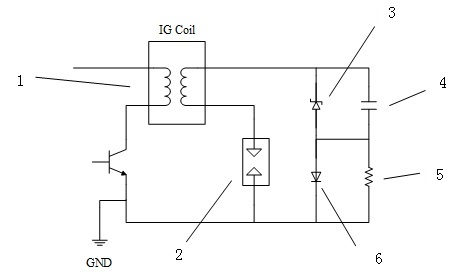
\includegraphics{thesis_figure/ion_struct}
	\caption{电容式离子电流检测电路结构}
	\label{fig:ionstruct}
\end{figure}
\par$1$表示点火线圈
\par$2$表示火花塞电极两段
\par$3$表示瞬态抑制二极管,防止电压过高使电路失效
\par$4$是电容,作为次级电路电源
\par$5$是检测电阻
\par$6$是普通二极管,用于限定检测电阻两端最大电压
\subsection{电容式离子电流曲线}
电容式离子电流分为三个时期:点火干扰期,火焰前锋期和火焰后期。如下图\ref{fig:ion_basic}所示是离子电流的三个时期。
\begin{figure}[!h]
	\centering
	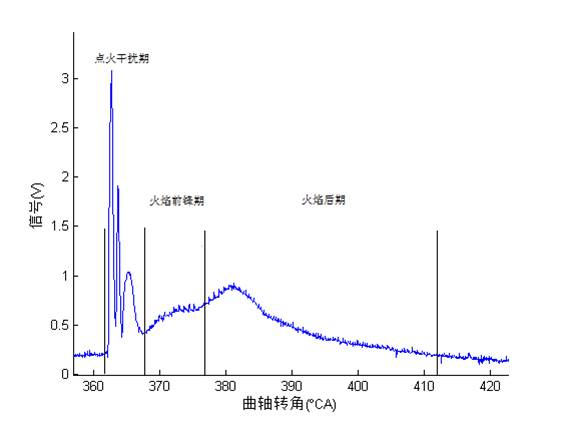
\includegraphics[width = 0.8\textwidth]{thesis_figure/model_chapter/ion_basic}
	\caption{电容式离子电流的三个时期}
	\label{fig:ion_basic}
\end{figure}
其中点火干扰期是由点火干扰造成的。火焰前锋期由火焰锋面经过电极附近的化学电离导致的;火焰后期由火焰锋面离开电极附近后的$NO$的热电离导致的。由于点火干扰的持续时间
和点火线圈的内部结构有关系,而火焰前锋期和火焰后期和燃烧有关系,所以点火干扰期可能会和火焰前锋期甚至是火焰后期相重合。但是点火干扰的曲线和火焰前锋或火焰后期的区别在于,点火干扰
期的曲线存在稳定的震荡信号,而化学电离或热电离导致的电流频率较低。通常来说火焰后期持续到整个燃烧阶段结束。
\subsection{火花塞动态电路模型}
火花塞结构复杂,但针对电磁干扰问题,主要考虑点火过程的放电通路,因此对其作适当的简化后的结果如图\ref{fig:hhsstruct}所示,其中金属外壳接地,具有耐高温、耐高压的氧化铝陶
瓷作为绝缘体,内置电阻由导电碳粉制成,中心电极为镍铜合金\cite{zyl2011}。
\begin{figure}[!h]
\centering
	\begin{minipage}[b]{0.5\textwidth}
		%\centering
		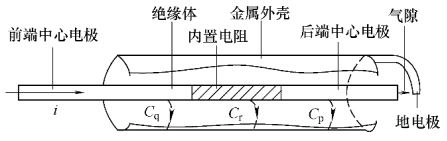
\includegraphics[width=\textwidth]{thesis_figure/anecdote_struct}
		\caption{火花塞内部放电通路}
		\label{fig:hhsstruct}
	\end{minipage}

	\begin{minipage}[b]{0.5\textwidth}
		%\centering
		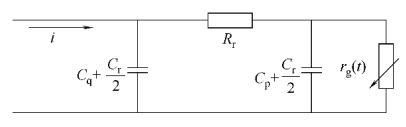
\includegraphics[width=\textwidth]{thesis_figure/anecdote_circuit}
		\caption{火花塞动态电路模型}
		\label{fig:hhscircuit}
	\end{minipage}
\end{figure}
其中$R_{r}$为火花塞内置电阻,其阻值可通过万用表测得或由生产商提供,通常为几千欧;$r_{g}$为火花塞气隙电阻,其阻值随火花塞的放电状态而发生变化,表征火花塞的非线性特性;
$C_{q}$、$C_{r}$、$C_{p}$分别表示前端中心电极、内置电阻、后端中心电极对火花塞金属外壳的寄生电容。火花塞内部可以看作静电场,因此火花塞动态模型可以如图\ref{fig:hhscircuit}所示。\
\subsection{火花塞间隙间的火花电阻}
图\ref{fig:hhscircuit}中的火花塞内置电阻$r_{g}$,前段中心电极对火花塞金属外壳的寄生电容$C_{q}$,内置电阻对火花塞金属外壳的寄生电容$C_{r}$,后端中心电极对火花塞
金属外壳的寄生电容$C_{p}$都可以通过有限元的方法进行计算\cite{zyl2011}。而火花塞间隙间的火花电阻$R_{g}$需要另外的方法进行计算。
\par由Rompe-Weizel理论可知,火花电阻$r_{g}$是一个随时间变化的量,当火花间隙被击穿后,其随时间变化的关系为:
\begin{equation}
	\label{eqn:qxr}
	r_{g}=l_{g}(\frac{2\alpha}{p\int_{\infty}i_{g}^{2}dt})^{-0.5}
\end{equation}
式中,$l_{g}$为间隙宽度;$a$为火花系数;$p$为混合燃气压力;$i_{g}$为流过间隙的火花电流。
\par间隙击穿后,火花电阻$r_{g}\leq5\Omega$,而火花塞电阻的阻值$5k\Omega\leq R_{r}\leq 20k\Omega$,所以$r_{g}\leq R_{r}$。考虑到高压点火导线的电阻$R_{w}$,火花
电流$i_{g}$主要有电容放电引起,根据电路理论可以得到:
\begin{align}
C &= C_{p}+\frac{C_{r}}{2}\\
\frac{du_{g}(t)}{dt}&=-\frac{1}{C}i_{g}(t)\\
\frac{di_{g}(t)}{dt}&=\frac{\alpha}{l_{g}^{2}p}u_{g}^{2}(t)i_{g}(t)-\frac{1}{C}\frac{i_{g}^{2}(t)}{u_{g}(t)}
\end{align}
设$t=t_{1}$时刻为电极产生电晕瞬间,$i_{g}(t_{1})=0$,$u_{g}(t_{1})=V_{br}$,$V_{br}$为火花塞气隙的击穿电压。利用数值算法,可以计算得到气隙电流$i_{g}(t)$及电压
$u_{g}(t)$。再代入式\ref{eqn:qxr}中即可求得$r_{g}$。
\subsection{离子电流检测电路等效电路模型}
根据火花塞的动态电路模型以及火花塞间隙间的火花电阻的计算公式,我们可以得到离子电流检测电路的等效电路模型如下:
\begin{figure}[!h]
	\centering
	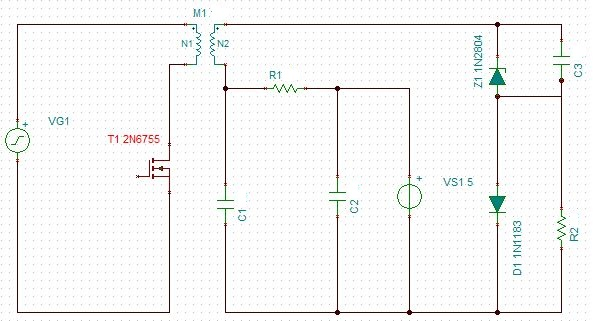
\includegraphics[width=0.8\textwidth]{thesis_figure/cmp_circuit}
	\caption{电路等效电路模型}
	\label{fig:cmp_circuit}
\end{figure}
\par其中$C_{1}=C_{q}+C_{r}/2$,$C_{2}=C_{p}+C_{r}/2$。由于火花塞间隙间的火花电阻$r_{g}$在不同时间的阻值不同,可以将该电路分为三种情况。
\subsubsection*{气隙断开的电路模型}
当MOSFET被点火控制信号触发后,在其导通时间内,一次线圈有电流通过,二次线圈出现感应电动势。但此时火花塞两极间的电压达不到击穿电压,此时火花塞气隙处于断开状态,此时在
MOSFET导通阶段有
\begin{gather}
	0\leq t\leq t_{1} \\
	r_{g}(t)=\infty \\                     
	i_{g}(t)=0
\end{gather}
时间$t_{1}$的计算即是计算火花塞气隙两段电压达到击穿电压$V_{br}$的时间。
\subsubsection*{气隙击穿瞬间的电路模型}
设火花塞气隙在$t=t_{1}$时开始产生电晕,$t=t_{2}$时被击穿,此过程火花塞由高阻抗特性变为低阻抗特性,即有
\begin{gather}
	t_{1}\leq t \leq t_{2}\\
	r_{g}=l_{g}(\frac{2\alpha}{p\int_{\infty}i_{g}^{2}dt})^{-0.5}
\end{gather}
\subsubsection*{气隙自持放电时的电路模型}
火花塞气隙击穿时出现电离现象,使得混合气被电离,从而形成了等离子通道,火花塞气隙进入自持放电阶段。此时火花塞两级电极间的电压维持稳定值
\cite{sincero2008arc,tseng1997experimentally},即有
\begin{gather}
	t_{2}\leq t \leq t_{3} \\
	u_{g}=U_{0}
\end{gather}
\section{小波分析}
\subsection{小波分析理论基础}
自从1822年傅里叶发表“热传导解析理论”以来,傅里叶变换一直是传统信号处理的基本方法。傅里叶变换能够满足大多数应用的需求,但是由于在进行
傅里叶变换的时候丢掉了时间信息,因此无法同时知道频域和时域情况下的信息。傅里叶变换在分析非平稳信号时表现出了严重的性能不足。然而实际中的信号
均包含大量的非平稳成分,比如突变、偏移等,然而这些非平稳信号往往反映了信号的重要特征。
\par为了研究信号在局部时间段的频域特征,1946年Gabor提出了著名Gabor变换,之后发展成为了短时傅里叶变换(STFT),其基本思想是对信号加窗,然后对窗
内的信号进行傅里叶变换,因此它可以反映出信号的局部特性。但由于STFT的定义决定了其窗函数的大小和形状与时间和频率无关,因此对低频信号采用大时间窗进行
分析,而对于高频信号用小时间窗进行分析。小波变换继承了STFT的思想,它的窗口大小不变,但窗口形状可以改变,是一种时间窗和频率窗都可变的时频分析方法, 
即在低频部分具有较高的频率分辨率和较低的时间分辨率,在高频部分具有较高的时间分辨率和较低的频率分辨率,因此在时频都具有很强的表征信号局部特征的能力。
\par在实际应用中,尤其是在计算机实现时,连续小波变换必须加以离散化,因此有必要讨论连续小波序列$\psi_{a,b}(t)$和连续小波变换$W_{f}(a,b)$的离散化。
在连续小波中,考虑小波函数
\begin{equation}
	\psi_{a,b}=|a|^{-\frac{1}{2}}\psi(\frac{t-b}{a})
\end{equation}
这里$b\in R$,$a\in R_{+}$,且$a\neq0$,$\phi$是容许的,为方便起见,在离散化中,总限制$a$只取正值,这样相容性条件就变为
\begin{equation}
	C_{\psi}=\int^{\infty}_{0}\frac{\mid \widehat{\psi}(\overline{\omega})\mid}{\mid \overline{\omega}\mid}d\overline{\omega} < \infty
\end{equation}
通常,把连续小波变换中尺度参数$a$和平移参数$b$的离散化公式分别取作$a=a_{0}^{j}$,$b=ka_{0}^{j}b_{0}$,这里$j\in Z$,扩展步长$a_{0}\neq 1$是固定值,
为方便起见,总是假定$a_{0}>1$(由于$m$可以取正也可以取负,因此这个假定无关紧要)。所以对应的离散小波变换函数$\psi_{j,k}(t)$即可写作
\begin{equation}
	\psi_{j,k}(t)=a^{-\frac{j}{2}}_{0}\psi(\frac{t-ka_{0}^{j}b0}{a_{0}^{j}})=a_{0}^{-\frac{j}{2}}\psi(a_{0}^{-\frac{j}{2}}t-kb_{0})
\end{equation}
而离散化小波系数则可表示为
\begin{equation}
	C_{j,k}=\int_{-\infty}^{\infty}f(t)\psi_{j,k}^{*}(t)dt=<f,\psi_{j,k}>
\end{equation}
其重构公式为
\begin{equation}
	f(t)=C\sum_{-\infty}^{\infty}\sum_{-\infty}^{\infty}C_{j,k}\psi_{j,k}(t)
\end{equation}
其中$C$是一个与信号无关的常数。由此可以看到信号序列$f(t)$可以由信号无关量$C$和小波函数$\psi$组成。
\subsection{多分辨率分析}
多分辨率分析是由一个尺度函数$\phi$建立起来的,因此多分辨率分析的建立等价于寻找尺度函数在多分辨率分析的框架下的性质。通过多分辨率分析可以从尺度函数$\phi$获得小波函数$\psi$,从而
可以对已知的信号进行分析和处理。
\par Mallat在1989年给出了计算小波函数$\psi$的理论方法:
\par设$(\{ V_{m};m\in Z\} ;\phi(t))$是一个正交多分辨率分析,则存在$\{ h_{k} \}\in l^{2}$使得下面的双尺度方程
\begin{equation}
	\phi(x) = \sum_{k}h_{k}\phi(2x-k)
\end{equation}
成立,并且利用尺度函数$\phi(x)$构造小波函数
\begin{equation}
	\psi(x)=\sum_{ki}g_{k}\phi(2x-k)
\end{equation}
其中$h_{k}=2\int_{-\infty}^{\infty}\phi(x)\overline{\phi(2x-k)}dx$,$g_{k}=(-1)^{k}\overline{h_{1-k}}$。
\par根据上述理论多分辨率分析可以得到离散化的尺度函数和小波函数的获得方法。
\subsection{小波函数分析步骤}
第一步是采样。如果待分解的是模拟信号$f(t)$,选择$N=2^{n}$,得到采样信号值$a_{k}^{n}=f(\frac{k}{2^{n}})$,其中$k$的取值保证$\frac{k}{N}$位于信号$f(t)$发生的时间范围
之内,并在每个不小于$\frac{1}{N}$的时间段内都能取到采样信号$a_{k}^{n}=f(\frac{k}{2^{n}})$,于是可以用信号
\begin{gather}
f_{n}(x)=\sum_{k\in Z}a_{k}^{n}\phi(2^{n}x-k)
\end{gather}
对连续信号$f(t)$进行高精度的近似。
\par第二步是分解。设信号$f_{n}(x)$逐级分解为
\begin{gather}
	f_{n}(x)=W_{n-1}(x)+W_{n-2}(x)+...+W_{l-1}(x)+f_{l-1}(x) \nonumber \\
			=W_{n-1}(x)+W_{n-2}(x)+...+W_{0}(x)+f_{0}(x)
\end{gather}
\par其中
\begin{gather*}
W_{l-1}(x)=\sum_{k\in Z}b_{k}^{l-1}\psi(2^{l-1}x-k)\\
f_{l-1}(x)=\sum_{k\in Z}a_{k}^{l-1}\psi(2^{l-1}x-k)
\end{gather*}
系数$a_{k}^{l-1}$与$b_{k}^{l-1}$按照上标
从大到小的顺序从$l=n$开始直到$l=0$结束,满足
\begin{gather}
	b_{k}^{l-1}=\frac{a_{2k}^{l}-a_{2k+1}^{l}}{2}\\
	a_{k}^{l-1}=\frac{a_{2k}^{l}+a_{2k+1}^{l}}{2}
\end{gather}
\par第三步是信号处理。将分解后的信号表示成下面的形式
\begin{gather}
	f_{n}(x)=\sum_{l=0}^{n-1}W_{l}(x)+f_{0}(x)\nonumber \\
			=\sum_{l=0}^{n-1}(\sum_{k\in Z}b_{k}^{l}\psi(2^{l}x-k))+\sum_{k\in Z}a_{k}^{0}\phi(x-k)
\end{gather}
信号处理的过程就是根据实际情况对$b_{k}^{l}$作适当的修正。例如信号处理的目的是去噪,那么可以将不可能存在的频率范围对应的系数$b_{k}^{l}$设置为0;如果信号处理用于压缩,则可以根据压缩比的
大小及小波系数的取值范围设置适当的阈值,当小波系数绝对值小于阈值时,设置$b_{k}^{l}$为零。
\par第四步是信号重构。设重构后的信号值满足
\begin{equation}
	\widetilde{f_{n}}(x)=\sum_{k\in Z}a_{k}^{n}\phi(2^{n}x-k)
\end{equation}
则上述信号值可以通过下面的递推过程得到
\begin{equation}
	\widetilde{a}^{l}=\widetilde{L}U\widetilde{a}^{l-1}+\widetilde{H}U\widetilde{b}^{l-1}, l=1,2,3,...,n
\end{equation}
其中$\widetilde{a}^{l}$和$\widetilde{b}^{l}$,$l=0,1,2,3,...,n$是根据第二、第三步得到的修正系数。
\subsection{小波分析的特点}
\begin{enumerate}[1)]
	\item\textbf{灵活性}\quad由于小波基函数$\phi(x)$不是唯一的,只需要满足构造小波函数的条件即可,因而就有许多构造小波的方法。不同的小波函数有不同的特性,可以用来逼近不同的信号
以便得到最佳结果。而傅里叶变换只用正弦信号逼近任意信号,没有选择的余地,逼近效果不能理想化。
	\item\textbf{快速性}\quad由于有了多分辨率分析,可以提高小波分析的效率。通过尺度函数和两尺度关系推导小波系数,在未知小波函数的解析表达式情况下也可以得到分析的结果。并且在频带细分下可以起到显微镜的作用,
这是傅里叶分析无法比拟的。
	\item\textbf{双域性}\quad小波分析是时频分析,可以时域和频域同时揭示信号的特征。而傅里叶变换只能在单域中显示信号特性。
	\item\textbf{深刻性}\quad小波理论是建立实变函数、复变函数、泛函分析、调和分析等近代数学理论基础上的,具有深刻的理论基础。
\end{enumerate}
\subsection{常见的可离散小波}
\par db小波的全称是Daubechies小波。Daubechies小波是由世界著明的小波分析学者Ingrid Daubechies构造的小波函数,我们一般简写成dbN,N是小波的阶数。小波函数$\psi(t)$和
尺度函数$\phi(t)$中的支撑区为2N-1,$\psi(t)$的消失矩为N。dbN小波具有较好的正则性,即该小波作为稀疏基所引入的光滑误差不容易被察觉,使得信号重构过程比较光滑。dbN小波的特点是随着阶次(序列N)的增大消失矩阶数越大,其
中消失矩越高光滑性就越好,频域的局部化能力就越强,频带的划分效果越好,但是会使时域紧支撑性减弱,同时计算量大大增加,实时性变差。另外,除N=1外,dbN小波不具有对称性(即非线性相位),即在对信
号进行分析和重构时会产生一定的相位失真。dbN没有明确的表达式(除了N=1外,N=1时即为Haar小波)。
\par symlet小波函数是Ingrid Daubechies提出的近似对称的小波函数,它是对db函数的一种改进。Symlet小波系通常表示为symN (N=2,3,…,8)。symN小波的支撑范围为2N-1,消失矩为N,同时也具备较好的正则性。该小波与dbN小波相
比,在连续性、支集长度、滤波器长度等方面与dbN小波一致,但symN小波具有更好的对称性,即一定程度上能够减少对信号进行分析和重构时的相位失真。
\par coiflet小波是根据R.Coifman的要求,由Daubechies构造的,它具有coifN (N=1,2,3,4,5)这一系列。Coiflet的小波函数$\psi(t)$的2N阶矩为零,尺度函数$\phi(t)$的2N-1阶矩为零。$\psi(t)$和$\phi(t)$的支撑长度为6N-1。
Coiflet的$\psi(t)$和$\phi(t)$具有比dbN更好的对称性。
\par dmey小波全称是discrete meyer小波,也就是离散meyer小波。meyer小波由法国数学家Yves Meyer于1990年提出。
\subsection{离散小波之间的比较}
在不同的应用领域,小波基的选取标准不同,一般的选择原则如下:
\par(1)正交性。正交性源于数学分析的简单和工程应用中便于理解操作,表现为小波基的可微性。
\par(2)紧支性。紧支集保证有优良的时频局部特性,也利于算法的实现。若小波函数$\psi(t)$有紧支集,则称小波基函数是紧支的。紧支集小波满足空间局部性的要求,特别在为了得到有限长度的滤波器组$h(n)$,$g(n)$
;避免滤波过程中的截断误差,要求小波基为紧支的。
\par(3)对称性。对称小波基具有线性相位特性,对图像边缘作对称边界扩展时,重构图像边缘部分失真较小,有利于复杂特性的分析。对称和反对称的尺度函数和小波函数是非常重要的,因为可以构造紧支的正则小波基,而且
具有线性相位。Daubechies已经证明,除了Haar小波基,不存在对称的紧支正交小波基。而对于双正交小波基,可以合成具有对称或反对称的紧支小波基。
\par(4)正则性。正则性是函数光滑程度的一种描述,函数频域能量的一种度量。正则性越高,小波分析效果越好。
\par(5)消失矩问题。为了提高衰减程度,要求所用的基函数具有一定的消失矩。消失矩的阶数越大,精细尺度下高频部分数据值就越有可能存在许多小至可以忽略的点。
下表\ref{tab:lsxb}所示的是所有的可以进行离散小波变换的小波比较\cite{wxf2003}。
\begin{table}[!h]
	\centering
	\caption{可离散变换的小波函数比较}
	\label{tab:lsxb}
	\begin{tabular}{c|c|c|c|c}
	\hline
	小波名称&正交性&双正交性&紧支撑性&支撑长度\\
	\hline
	db&是&是&是&2N-1\\
	sym&是&是&是&2N-1\\
	dmey&是&是&是&有限长度\\
	coif&是&是&是&6N-1\\
	\hline
	\multicolumn{5}{c}{}
	\end{tabular}
	\begin{tabular}{c|c|c|c|c}
	\hline
	小波名称&滤波器长度&对称性&小波函数消失矩阶数&尺度函数消失矩阵数\\
	\hline
	db&2N&对称&N&-\\
	sym&2N&近似对称&N&-\\
	dmey&[-8,8]&对称&-&-\\
	coif&6N&近似对称&2N&2N-1\\
	\hline
	\end{tabular}
\end{table}
基本小波类型的选择较难总结成一般原则,只能针对具体问题提出具体原则。例如对于分段多项式结构组成的信号,db小波比较适用;如果信号含正弦分量或高频振荡,则局部三角函数基比较合适。如何
根据分析信号的特点,结合任务来优化设计小波函数一直是值得探讨的问题,迄今为止还没有系统完整的总结。且对于一些特定的离散问题,还可以通过利用多分辨率分析的方法自己构造离散的尺度函数和
小波函数。
\section{高斯曲线拟合}
\subsection{高斯函数}
高斯函数的应用范围很广,在自然科学、社会科学、数学以及工程学等领域都能看到它的身影。高斯函数的形式为:
\begin{equation}
	f(x)=ae^{-\frac{(x-b)^2}{c^2}}
\end{equation}
其中$a$,$b$,$c$为实常数,且$a>0$。
\par $c^2=2$的高斯函数是傅里叶变换的特征函数。这就意味着高斯函数的傅里叶变换不仅仅是另一个高斯函数,而且是进行傅里叶变换的函数的标量倍。
高斯函数的不定积分是误差函数。在自然科学、社会科学、数学以及工程学等领域都有高斯函数的身影,比如在统计学与机率论中,高斯函数是正态分布的密度函数,根据中心极限定理,他是复杂
总和的有限几率分布。
\subsection{离子电流拟合原理和方法}
Saitzkoff\cite{saitzkoff1996ionization}在缸内气体完全燃烧并且达到热化学平衡情况下推导了火焰后期的离子电流的理论公式。
\begin{equation}
	\frac{I}{I_{m}}=\frac{1}{\frac{p}{p_m}}^{\frac{1}{2}-\frac{3}{4}\frac{\gamma -1}{\gamma}}e^{-\frac{E_i}{2\kappa T_m}[\frac{1}{(\frac{p}{p_m})^{\frac{\gamma -1}{\gamma}}}-1]}
\end{equation}
其中各物理量含义如下所示\par
\begin{table}[H]
	\centering
	\begin{tabular}{cc}
	I&离子电流\\
	$I_m$&离子电流最大值\\
	p&缸压\\
	$p_m$&缸压最大值\\
	$T_m$&最大温度\\
	$\gamma$&热力学系数\\
	$\kappa$&波尔兹曼常数\\
	$E_i$&离子电流能量
	\end{tabular}
\end{table}
\par该公式与高斯函数相近。所以整个离子电流的计算公式可以写成
\begin{gather}
	I(\theta)=f(\theta)+\alpha_{1}e^{-\frac{1}{\alpha_{2}}(\theta - \alpha_{3})^2} \label{eqn:interp1}
\end{gather}
其中$f(\theta)$是火焰前锋期的模型。为了简化整个模型的计算,我们可以将火焰前锋期的模型也有高斯函数替代。于是整个离子电流的计算公式写成
\begin{gather}
	I(\theta)=\alpha_{1}e^{-\frac{1}{\alpha_{2}}(\theta - \alpha_{3})^2}+\beta_{1}e^{-\frac{1}{\beta_{2}}(\theta - \beta_{3})^2}
	\label{eqn:interp2}
\end{gather}
L.Eriksson和L.Nielsen\cite{eriksson1996ignition,eriksson1997closed,eriksson1997ionization}采用该方法能够准确地估计缸压最值对应相位,从而可以
自适应调整点火提前角,提高了发动机的燃烧效率。





% !TeX encoding = GB2312
\chapter{����ʽ���ӵ�������·ʵ��̨��}
\section{ʵ��̨��}
��ʵ��̨���ɷ�������������֧�ܣ����������Ӻ����������豸��ɡ���̨��ϵͳʾ��ͼ��\ref{fig:platformintro}ͼ��ʾ��
\begin{figure}[!h]
	\centering
	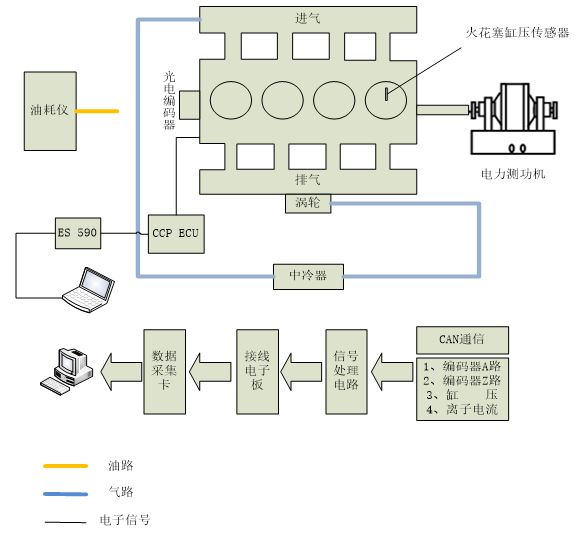
\includegraphics[width=0.85\textwidth]{thesis_figure/platformer_chapter/platformer_intro}
	\caption{̨��ϵͳʾ��ͼ}
	\label{fig:platformintro}
\end{figure}
���з������Ǵ����ڳ����1.8T��������ѹ�����������䷢�����������⹦��Ϊ�Ϸ�⹦�����ͺ���ΪAVL�ͺ��ǣ�ͨ��Kistler����ʽ��ѹ��������������ѹ���ù�������
��ͬ���źŲ�ȷ��������ֹ��λ�á�ͨ��������ͨ�ĵ����Ȧ��������Ȧ��ѹ��ͽӵص�������ӵ����ɼ���·�����ɼ����ӵ����źš���ʵ��ͼ��ͼ\ref{fig:platformintro_real}��ʾ��
\begin{figure}[t]
	\centering
	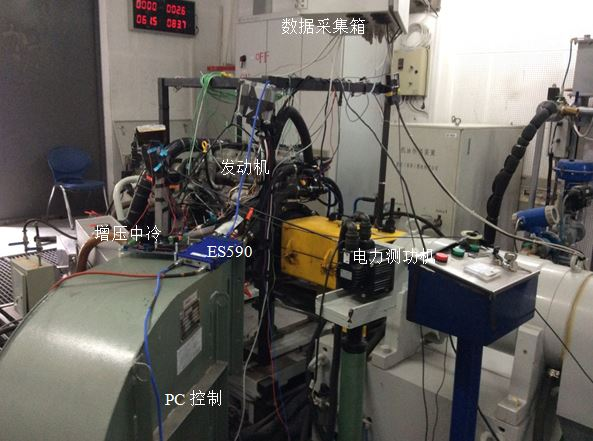
\includegraphics[width=0.8\textwidth]{thesis_figure/platformer_chapter/platformer_intro_real}
	\caption{̨��ϵͳʵ��ͼ}
	\label{fig:platformintro_real}
\end{figure}
\subsection{������}
������Ϊ�����ڳ����1.8T�ϵ�������ѹPFI����������ʵ��ͼ��\ref{fig:ecu}��ʾ�������������\ref{tab:ice}��ʾ��
��ECUΪ���������������޹�˾�ṩ�Ļ���ME788����ϵͳ��ECU��ʵ��ͼ��ͼ\ref{fig:ice}��ʾ��
\begin{figure}[!ht]
	\begin{minipage}[h]{0.5\linewidth}
		\centering
		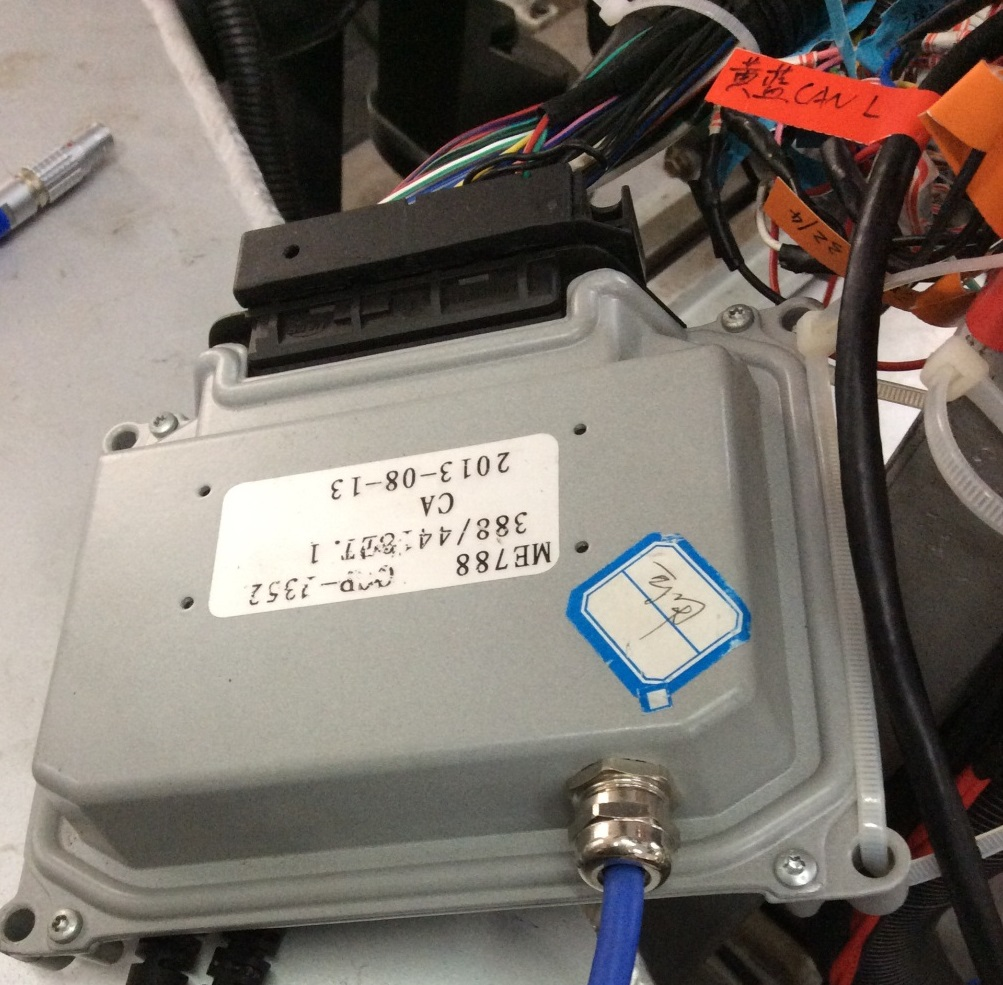
\includegraphics[width=0.8\textwidth]{thesis_figure/platformer_chapter/ecu}
		\caption{ECUʵ��ͼ}
		\label{fig:ecu}
	\end{minipage}
	\begin{minipage}[h]{0.5\linewidth}
		\centering
		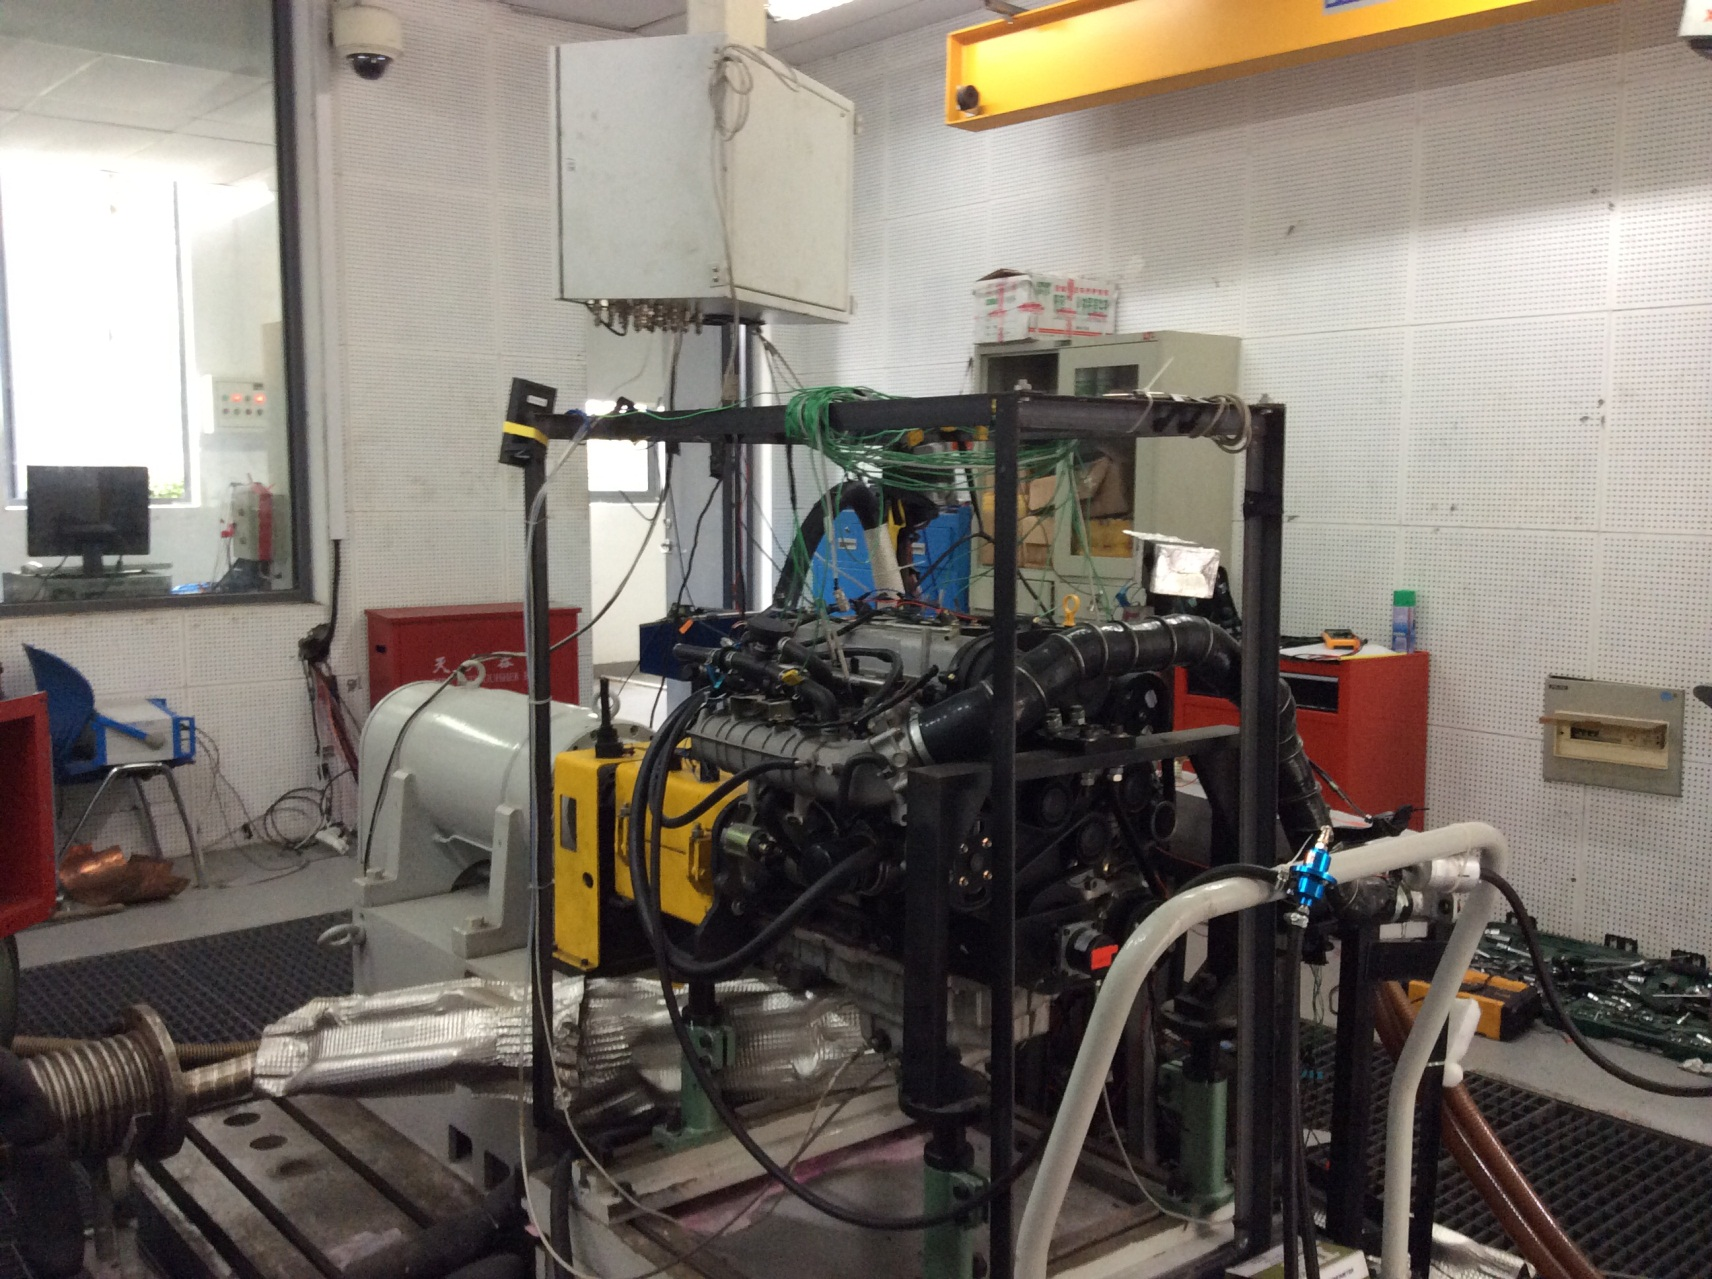
\includegraphics[width=\textwidth]{thesis_figure/platformer_chapter/ice}
		\caption{������ʵ��ͼ}
		\label{fig:ice}
	\end{minipage}
\end{figure}
\begin{table}[ht]
	\centering
	\caption{�������������}
	\label{tab:ice}
	\begin{tabular}{c|c}
		\hline
		���������� & 4���PFI������ѹ������ \\\hline
		����(cc) & 1798 \\\hline
		�����(kW) & 130 \\\hline
		���Ť��(Nm) & 230 \\\hline
		�׾�(mm) & 86 \\\hline
		�г�(mm) & 77.4 \\\hline
	\end{tabular}
\end{table}
\parͨ��INCA����������ECU��������ʾ�������������MDA�Ա�������ݽ��м򵥵����ݷ�����

\subsection{������֧��}
������֧����Ҫ�ɷ�������װ�ƽ̨�Ϳɵ�����֧����������ɡ��÷�������װ�ƽ̨�ɿ�ܡ���ĥ���졢�߾���
��λװ�á�����װ�á�������������ĥ���س��ּ������̵���ɣ�ʵ���ͼ\ref{fig:hdpt}���û��װƽ̨ͨ���߾��ȶ�λ������֤
ƽ̨�ĺ����������룬��֤�˹̶��ڸûƽ̨�ϵķ��������ԺͲ⹦���ķ����νӴ��ľ��ȣ�ͬʱ����˸ûƽ̨�ĸ����ԣ��Ӷ�
��Ч�ؼ����˷�������װ�͵�����ռ�õ�ʱ�䡣������֧����ת�ӹ�װ��ZJϵ�пɵ�֧�ܡ���������ɣ�������30��800KW��������֧��
Ҫ��ͬʱ���˻ƽ̨�кܸߵļ����ԣ����ڶ��ַ����������ã�����ʵ�ַ���������λ������
\begin{figure}[!h]
	\begin{minipage}[h]{0.5\linewidth}
		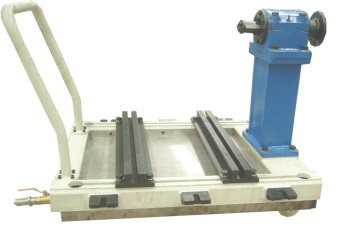
\includegraphics[width=0.8\textwidth]{thesis_figure/platformer_chapter/hdpt}
		\caption{��������װ�ƽ̨}
		\label{fig:hdpt}
	\end{minipage}%
	\begin{minipage}[h]{0.5\linewidth}
		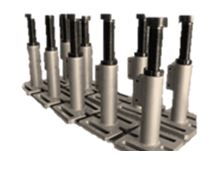
\includegraphics[width=0.8\textwidth]{thesis_figure/platformer_chapter/lxzj}
		\caption{�ɵ�����֧��}
		\label{fig:ktzj}
	\end{minipage}
\end{figure}
\par�ɵ�����֧���ɻ�ļ���˺�T�͵�����������ɣ�ʵ���ͼ\ref{fig:ktzj}��������֮��ͨ�����ƿ����ӡ�T�͵��������ڷ�������װ�ƽ̨����ĥ������
��С�������˶���ͨ��������˨���Թ̶������λ�á�����˲��ý�Ϊ�����Ľ����������ɣ���ͨ���ڰ�װ�����������ϵ���һЩ����Ƭ��߼���
Ч��������˶��������ƿף����㷢����֧����֮�̶���
\begin{figure}[h]
	\centering
	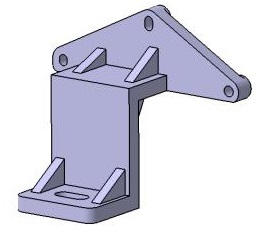
\includegraphics[width=0.3\textwidth]{thesis_figure/platformer_chapter/zj1}
	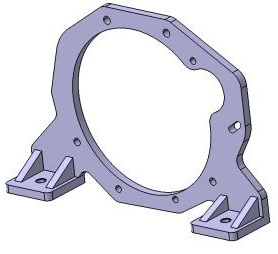
\includegraphics[width=0.3\textwidth]{thesis_figure/platformer_chapter/zj2}
	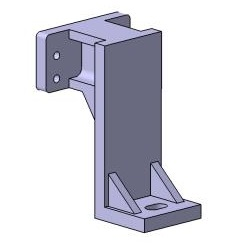
\includegraphics[width=0.3\textwidth]{thesis_figure/platformer_chapter/zj3}
	\caption{������֧�ܲ���ͼ}
	\label{fig:zjbjt}
\end{figure}
\par�������ϵ����ֻ����ṹ������˸Ŀ������֧�ܽṹ��ѡ�񷢶����������ϱ�����Ϊ������׼ˮƽƽ�棬ѡ����ֶ�ƽ��Ϊ��׼��ֱ�棬����ˮƽ�ߡ�ֱ�dzߺ�
�α꿨�ߵ����߲����̶�����������˨�����׼���Ŀռ���롣ʹ��CATIA��ά��е���������˷�����֧�ܵ���άģ�ͣ�������װ�䵽���ⷢ����ģ���ϡ�
���ֶ�֧�ܲ�������ʽ�ṹ���㹻���ܾ������ϵ�Ľ����غɣ�ͨ�����Ӽ�ǿ���밲װ�̶����ķ�ʽ����֤����ʱ�����˵�����֧�ܽṹ���գ�ͬʱ��ֿ����ŶȺ�
����������������������������������ģ������֧�ܲ��������֧����ơ�����֧�ܺ��Ӳ���ƴ�ӹ��գ�ÿ��������ʹ������λֱ���棬���ӹ����۽��������֧���ں�
�Ӻ�������α䡣��ͼ\ref{fig:zjbjt}��ʾ��
\subsection{�⹦��}
���������⹦����Ŀǰ�г������Ƚ��Ķ������ز����豸����ɼ�˸�������е���׼����ٵļ��ز⹦ʵ�飬�����ܡ��ɿ��Լ�ά�����׳̶ȵȷ��涼�бȽ����Ե����ơ�
����ʵ����õĽ��������⹦��ϵͳ���Կ������������������޹�˾���ò⹦��ϵͳ�����Ƚ���Ƶ����ƽ̨����������е͹��ԡ��߾��ȡ����ȶ��ԡ��ṹ�򵥡�ά����
�㡢�Գ�ϵ�в������ڲ��������Զ������ŵ㡣��ͼ\ref{fig:dlcgj}�Dz⹦����װ���ߵ�ʾ��ͼ��
\begin{figure}[H]
	\centering
	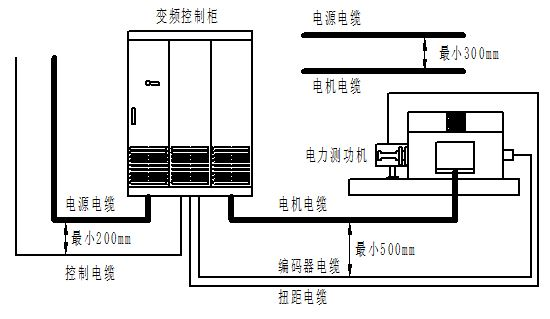
\includegraphics[width=0.5\textwidth]{thesis_figure/platformer_chapter/dlcgj}
	\caption{DCWϵ�н��������⹦��ϵͳ��װ����ʾ��ͼ}
	\label{fig:dlcgj}
\end{figure}
\par�ý��������⹦����Ҫ��һ̨�����첽������������߾���ת�ٱ�����������Ť�ط�������һ�׿����������еĽ������ٹ񡢿���ϵͳ���ɼ�ϵͳ��ɡ�������Ƶ���ٹ��Ϊ����
��Ԫ����䵥Ԫ��������ɡ�������Ԫ�Ŀɿع轫�û������380V������ת��Ϊ�ڲ�֮���㣬��ֱ���������Ϊ��ѹ��Ƶ�ʿɱ�Ľ���������������첽�����
\begin{figure}[H]
	\centering
	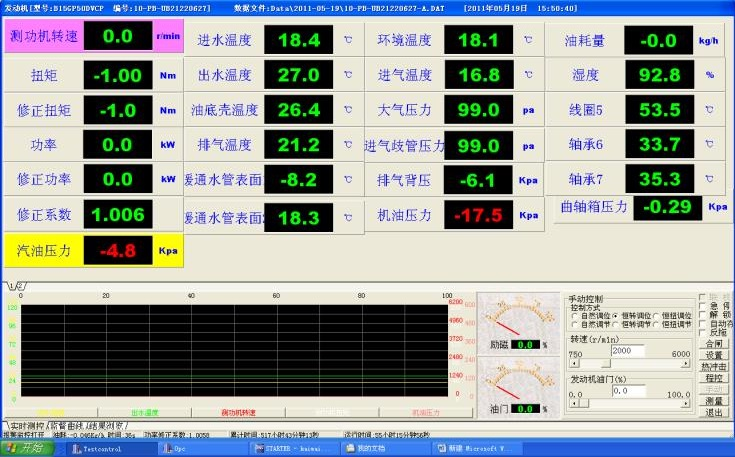
\includegraphics[width=0.8\textwidth]{thesis_figure/platformer_chapter/cgjkzjm}
	\caption{�⹦�����ƽ���}
	\label{fig:cgjkzjm}
\end{figure}

\begin{figure}[H]
	\centering
	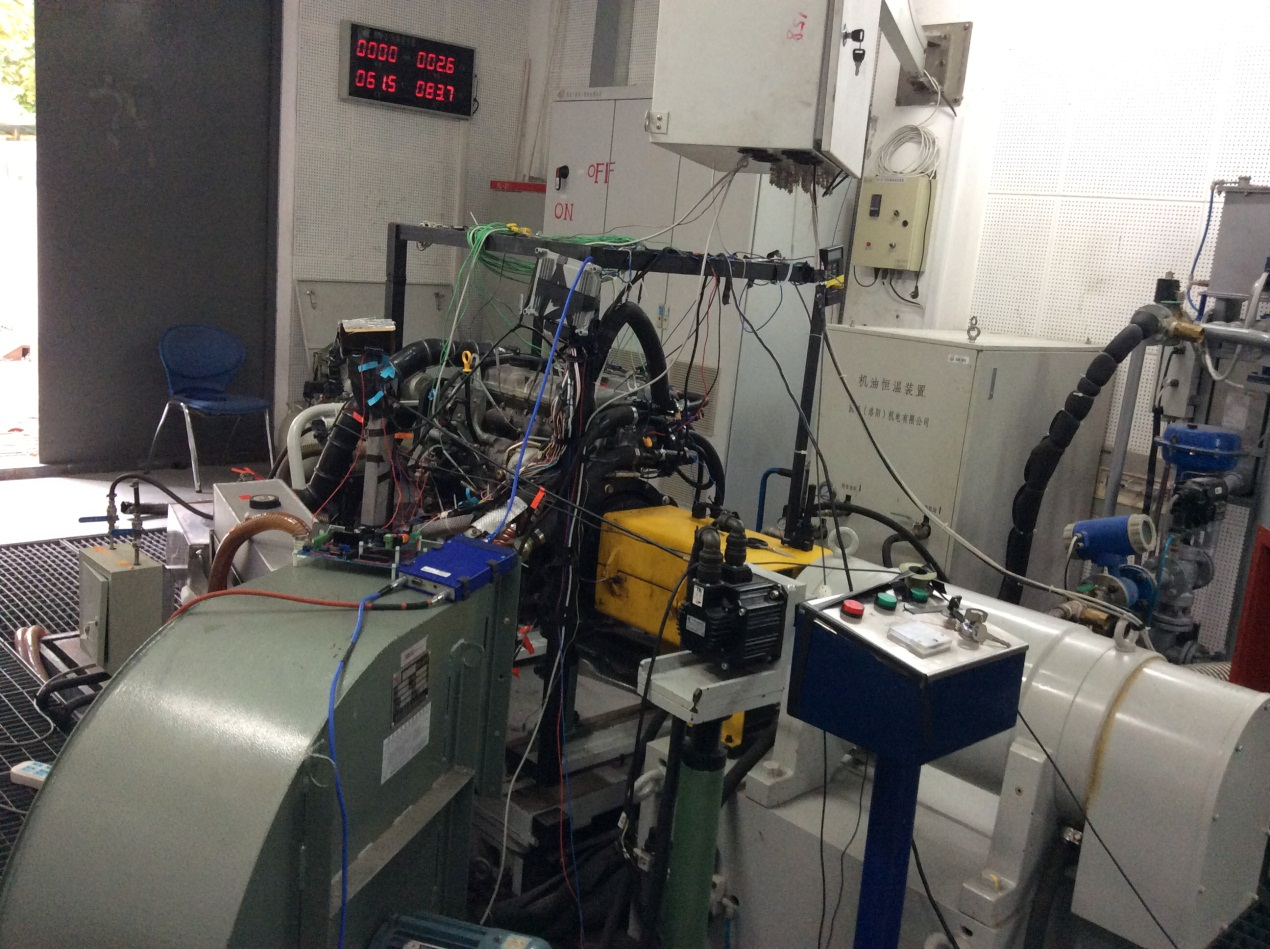
\includegraphics[width=0.65\textwidth]{thesis_figure/platformer_chapter/dlcgjswt}
	\caption{�����⹦��ʵ��ͼ}
	\label{fig:dlcgjswt}
\end{figure}
\par�⹦����ʵ��ͼ��\ref{fig:dlcgjswt}��ʾ�������������\ref{tab:dlcgjjtcs}��ʾ�����϶�״̬ʱ��ͨ�������������Ƶ�ʼ���ѹ�Ըı�ת�٣��ﵽ�϶����ص�Ŀ�ģ��ڷ���״̬ʱ��ͨ�������������ת��������������Ľ�����ת��Ϊֱ�����پ���������Ԫת��
Ϊ��������Ҫ��Ľ����磬�����������Դﵽ����ת�ص�Ŀ�ġ��⹦�����ƽ�����ͼ\ref{fig:cgjkzjm}��ʾ���ý���ʵʱ��ʾ̨�����������ת�١�ˮ�¡�Ť�ص�״̬��
���������м�ͣ���ܡ�
\begin{table}[H]
	\centering
	\caption{�����⹦���������}
	\label{tab:dlcgjjtcs}
	\begin{tabular}{ccc}
	\hline
	�������� & ������Χ & ����\\\hline
	ת�� & $0\thicksim10000r/min$ &$\pm 1 r/min$ \\
	Ť�� & $0\thicksim500N\centerdot m$ &$\pm 0.4 \%FS$ \\
	ȼ������ &$0\thicksim100Kg/h$ & $\pm 0.12\% FS$ \\
	�����¶� &$0\thicksim50^{\circ}C$ & $\pm 0.5\% FS$ \\
	����ʪ�� &$0\thicksim100\%$ & $\pm 2\% RH$ \\
	��ȴˮ���� &$0\thicksim150^{\circ}C$ & $\pm 0.5^{\circ}C$ \\
	��ȴˮ���� &$0\thicksim150^{\circ}C$ & $\pm 0.5^{\circ}C$ \\
	�����¶� &$0\thicksim150^{\circ}C$ & $\pm 0.5^{\circ}C$ \\
	ȼ���¶� &$0\thicksim150^{\circ}C$ & $\pm 0.5^{\circ}C$ \\
	����ǰ�¶� &$0\thicksim150^{\circ}C$ & $\pm 0.5^{\circ}C$ \\
	������¶� &$0\thicksim250^{\circ}C$ & $\pm 0.5^{\circ}C$ \\
	�����¶� &$0\thicksim150^{\circ}C$ & $\pm 0.5^{\circ}C$ \\
	����ѹ�� &$0\thicksim1000KPa$ & $\pm 0.5\%FS$ \\
	ȼ��ѹ�� &$0\thicksim1000KPa$ & $\pm 0.5\%FS$ \\
	��ˮѹ�� &$0\thicksim600KPa$ & $\pm 0.5\%FS$ \\
	��ˮѹ�� &$0\thicksim600KPa$ & $\pm 0.5\%FS$ \\
	������ѹ�� &$-20\thicksim20KPa$ & $\pm 0.25\%FS$ \\
	������ѹ &$0\thicksim50KPa$ & $\pm 0.5\%FS$ \\
	����ǰѹ�� &$0\thicksim300KPa$ & $\pm 0.5\%FS$ \\
	�����ѹ�� &$0\thicksim300KPa$ & $\pm 0.5\%FS$ \\
	����ѹ�� &$80\thicksim110KPa$ & $\pm 0.25\%FS$ \\\hline
	\end{tabular}
\end{table}
\subsection{����������}
����������������ѹ����ϵͳ����ȴϵͳ��������ϵͳ�ȡ�
\par\textbf{��ѹ����ϵͳ}
\par��ѹ����ϵͳ������������������������ˮ����ˮ����ѹѹ���¶ȴ������Ȳ�����ɣ�ʵ��ͼ��ͼ\ref{fig:zyzlq}��ʾ��
\begin{figure}[H]
	\centering
	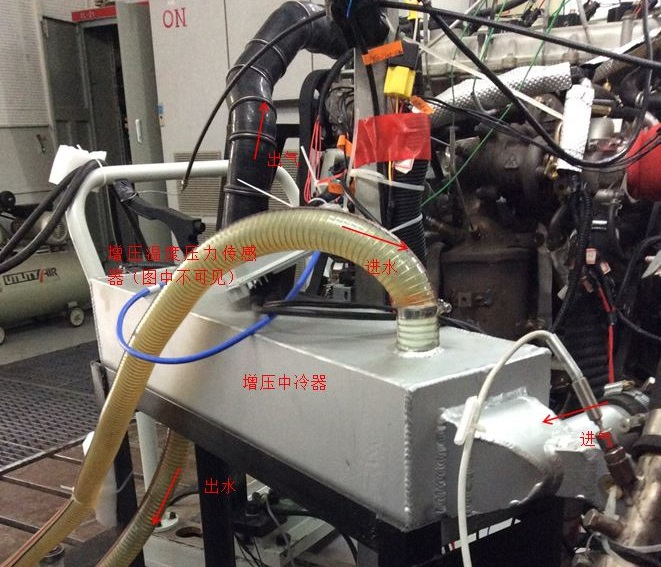
\includegraphics[width=0.7\textwidth]{thesis_figure/platformer_chapter/zyzlq}
	\caption{��������ѹ����ϵͳ}
	\label{fig:zyzlq}
\end{figure}
\par\textbf{��ȴϵͳ}
\par��ȴϵͳ��Ϊˮ��ͷ��������֣�ˮ������ӵ���ȴѭ��ϵͳ���ɣ���ͼ\ref{fig:sllqxt}��ʾ����������Ҫ��ʹ�ô�
�ʵķ���������ܣ�ʵ�ֿ��ٽ��£�ʹ�¶�����Ҫ��Χ֮�ڣ���ͼ\ref{fig:fllqxt}��ʾ��
\begin{figure}[H]
	\centering
	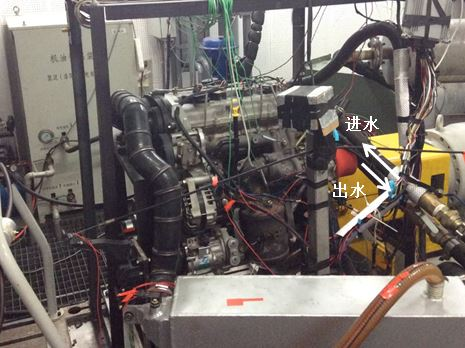
\includegraphics[width=0.7\textwidth]{thesis_figure/platformer_chapter/sllqxt}
	\caption{���������ˮ��ϵͳ}
	\label{fig:sllqxt}
\end{figure}
\begin{figure}[H]
	\centering
	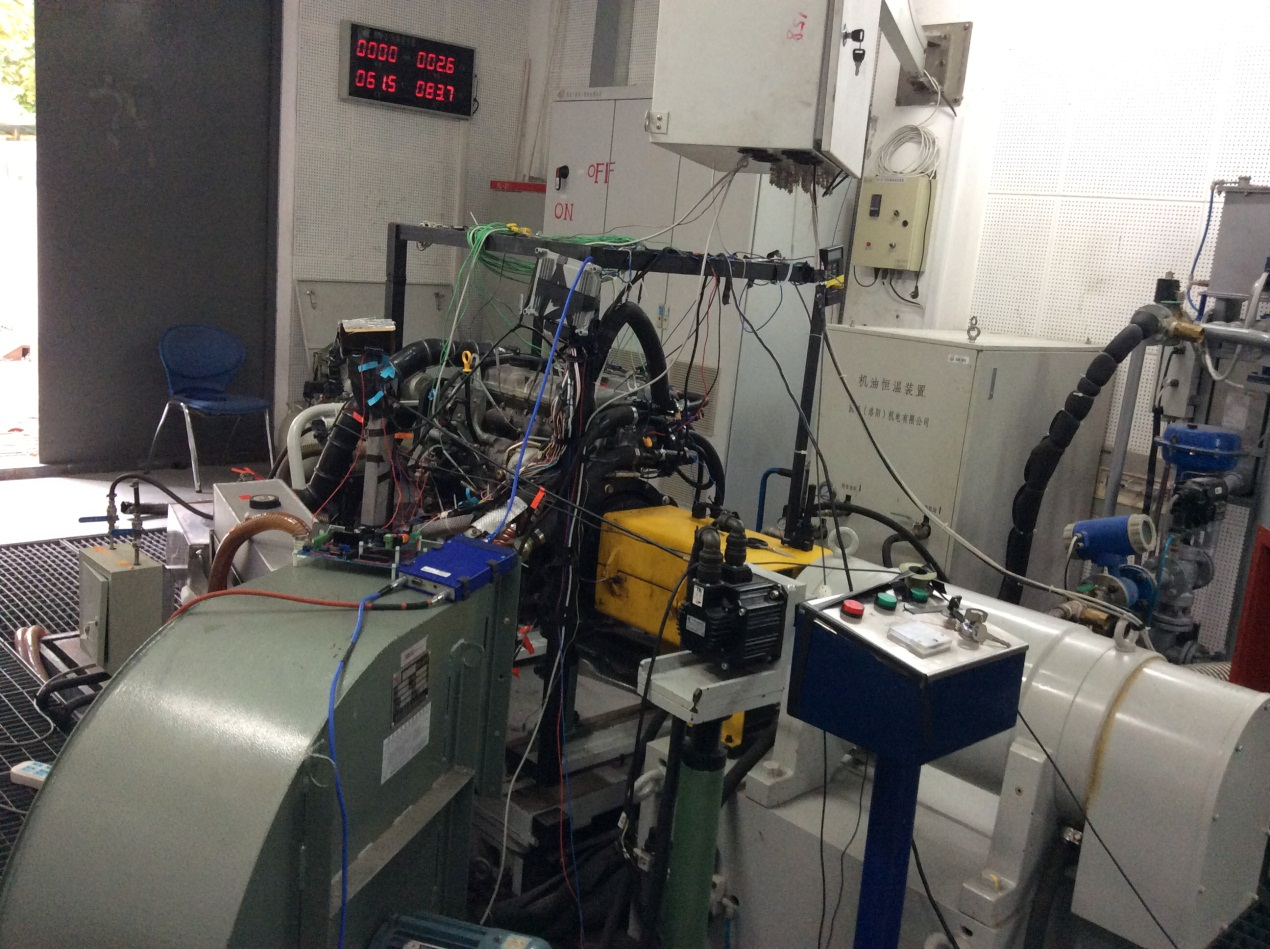
\includegraphics[width=0.7\textwidth]{thesis_figure/platformer_chapter/fllqxt}
	\caption{��������ӷ���ϵͳ}
	\label{fig:fllqxt}
\end{figure}
\par\textbf{������ϵͳ}
\par����ϵͳ�����ƿ�����������ԭ����������ɣ�����ϵͳ��ԭ��������ܡ������ܼ�������һ��������ͨ��ʵ��������ϵͳ�У�
���У���������װ�������¶ȴ�����������ϵͳ��ͼ\ref{fig:jpqxt}��ʾ��
\begin{figure}[H]
	\centering
	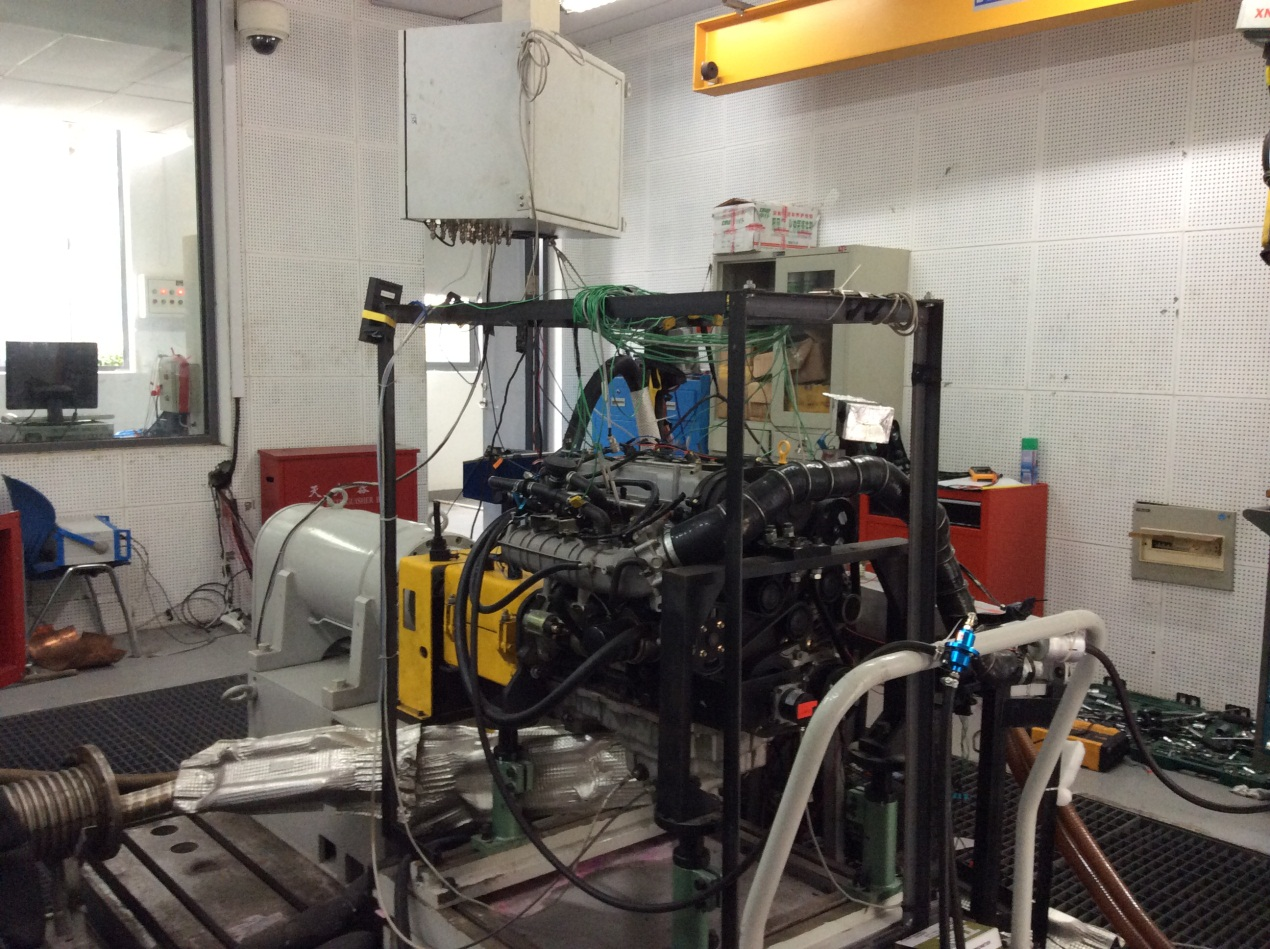
\includegraphics[width=0.7\textwidth]{thesis_figure/platformer_chapter/jpqxt}
	\caption{������������ϵͳ}
	\label{fig:jpqxt}
\end{figure}
\section{ʵ���豸������}
\subsection{��ѹ������}
��ѹ���������õ���KISTLER �ṩ��6118B�ͻ�����ѹ������������������3mm��ѹ�������Ϳɻ����£����������׼���ʵ
�ָ�ѹ�IJ�����
\begin{table}[H]
	\caption{��ѹ�������������}
	\label{tab:gycgq}
	\centering
	\begin{tabular}{ccc}
	\hline
	������ & ��λ& ��ֵ \\
	\hline
	���� & g& 50\\
	ѹ����Χ & bar & $0\thicksim 200$ \\
	�궨����(��200$^{\circ}C$) &bar & $0\thicksim 150$ \\
	���� & bar & 250 \\
	������(200$^{\circ}C$) & pC/bar & $\thickapprox10$ \\
	����Ƶ�� & kHz & $>100$ \\
	�������Զ� & \%FSO & $\leq \pm$ 0.5 \\
	���ٵ������ȣ�����;��� & bar/g & $<0.005$ \\
	�����������¶ȷ�Χ & $^{\circ}C$ & $-20\thicksim 350$ \\
	���¹����¶ȷ�Χ & $^{\circ}C$ & $-20 \thicksim 200$ \\
	�����ȱ仯($200\pm 50^{\circ}C$)&\%& $\leq\pm 1$ \\
	����Ʈ��$\triangle p$ & bar & $\leq \pm 0.6$ \\
	$\triangle p_{min}$ & \% & $\leq \pm 3$ \\
	$\triangle p_{max}$ & \% & $\leq \pm 1.5$ \\
	20$^{\circ}C$ʱ��������Ե�迹 & $\Omega$ & $>1013$ \\
	200$^{\circ}C$ʱ��������Ե�迹 & $\Omega$ & $>1011$ \\
	�����迹(1000V��������) & $\Omega$& $>100$ \\
	��Եǿ�� & kV& $<35$ \\
	���������� & pF/m& 110\\
	\hline
	\end{tabular}
\end{table}
��װ����������С��ѹ��ʽ���¸�ѹ����������װʱ��ǰ����ȼ�����ڲ�ƽ�룬����Ƶ�ʸ���100kHz����ˣ�Ҳ����
�ڸ��ٷ������ͱ�����Ʋ��ԡ���ʵ��ͼ�ͼ���������ͼ\ref{fig:gycgq}�ͱ�\ref{tab:gycgq}���仹�䱸��װ������ʽ˫
ͨ����ɷŴ���ģ����źŵ���ƽ̨���źŷŴ�ΧΪ$\pm 100\thicksim 10000$pc/V��ͨ�����Ŵ�������ѹ���źŴ�
�����ػ��ɼ�����¼����ȼ��ѹ�����ݡ�
\par���ֵ�ɷŴ�����������ʵ����ͨ��ѹ������Dz�������Ť�ء�ͨ������������ѹ�紫�����ϲ���һ���������仯�ĵ�ɡ���
������źŷŴ���ת���ɱ����������ѹ����ɷŴ�����ʵ��ͼ��ͼ\ref{fig:gycgqdhfdq}��ʾ��
\begin{figure}[ht]
	\begin{minipage}[H]{0.5\linewidth}
		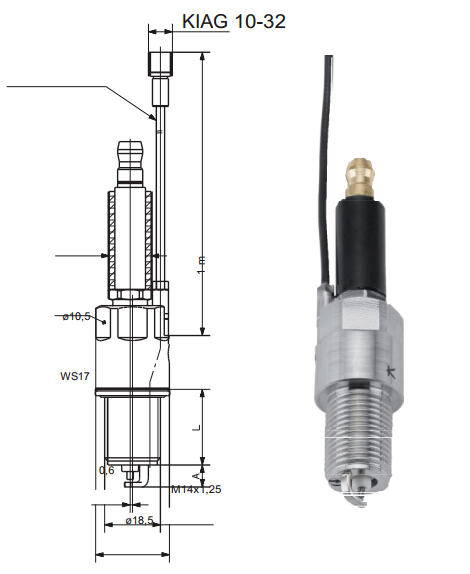
\includegraphics[width=0.8\textwidth]{thesis_figure/platformer_chapter/gycgq}
		\caption{����ʽ��ѹ������}
		\label{fig:gycgq}
	\end{minipage}
	\begin{minipage}[H]{0.5\linewidth}
		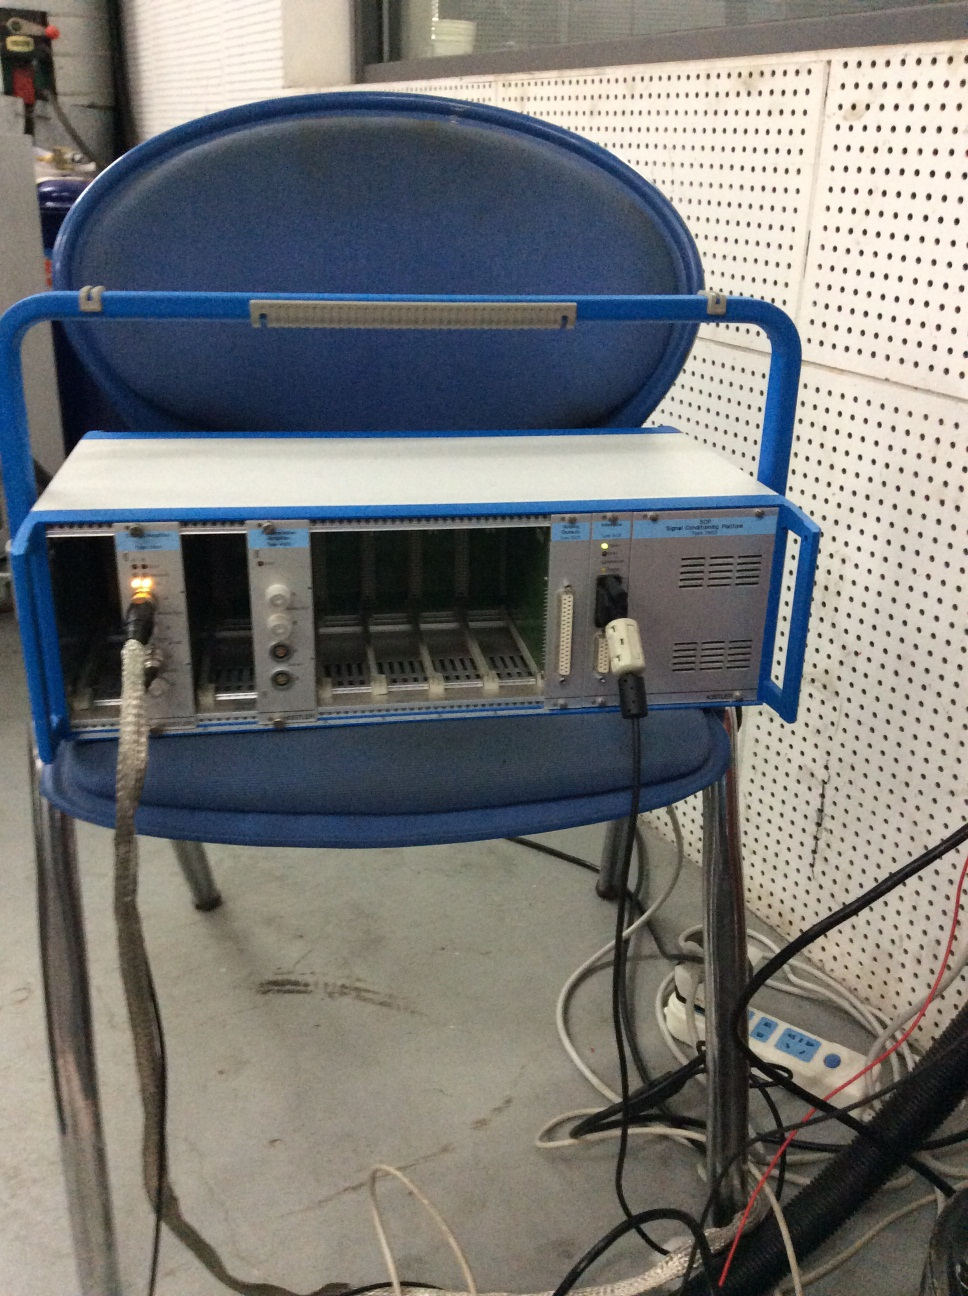
\includegraphics[width=0.8\textwidth]{thesis_figure/platformer_chapter/gycgqdhfdq}
		\caption{��ѹ��������ɷŴ���}
		\label{fig:gycgqdhfdq}
	\end{minipage}
\end{figure}
\subsection{��������}
��������ʱ����������˰�װHGAIN��˾��F5809������ʽ���������������źŲ�����Χ720 pulse/r����������$0.5^{\circ}CA$����
ͼ\ref{fig:gdbmq}��ʾ���ñ������ڲ�����ASIC�������������������ɿ��Ըߣ��źŷֱ��ʸߣ�������������ǿ���źŴ������ϳ����ŵ㣬Ϊ
�ɼ����ṩ�����жϱ�֤����A·��Z·�ź����ڸ��ٲɼ�ϵͳ����Դ�Լ���Ϊ�������ݴ���������ʱ�̲ο����ݡ�
\begin{figure}[H]
	\centering
	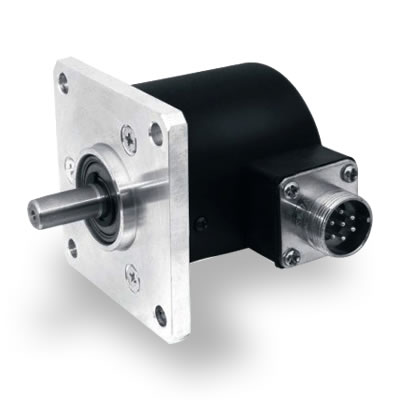
\includegraphics[width=0.4\textwidth]{thesis_figure/platformer_chapter/gdbmq}
	\caption{��������}
	\label{fig:gdbmq}
\end{figure}
\subsection{�ɼ���}
���ݲɼ�ϵͳ������ʵʱ���������淢�������й����и�˲̬�����ġ����������NI��˾��Ʒ��PCI 6250���ٲɼ�������߱�16·ģ���ź����룬16
λת�����ȣ���ͨ������Ƶ��1MHz����ͨ��ģʽ��1.25MHz�����ɼ���ֵ��ΧΪ��10V��ǿ���ܡ�\par�о����𹤿��µ����ӵ���������Ҫ�ɼ��IJ���
��Ϊ�����ࣺ��һ���Ƿ�ӳ�����ڲ�ȼ��״̬���ŷŵ��źţ������ȼ��ѹ���źš����ӵ����źż������ж�������λ��A·��Z·�źŵȣ����Ƿ�����
ECUͨ��CAN���߷��ͳ���������״̬�����źţ��緢����ת�١����������ɡ��������ֵ�������¶ȡ�����ѹ������ȴˮ�¶��Լ�����ѹ���ȵȡ��ò�
�����ܹ����������������󡣲ɼ���ʵ��ͼ��ͼ\ref{fig:nicjk}��ʾ�����ڿ�����Ϊ�˸�����š�
\begin{figure}[H]
	\centering
	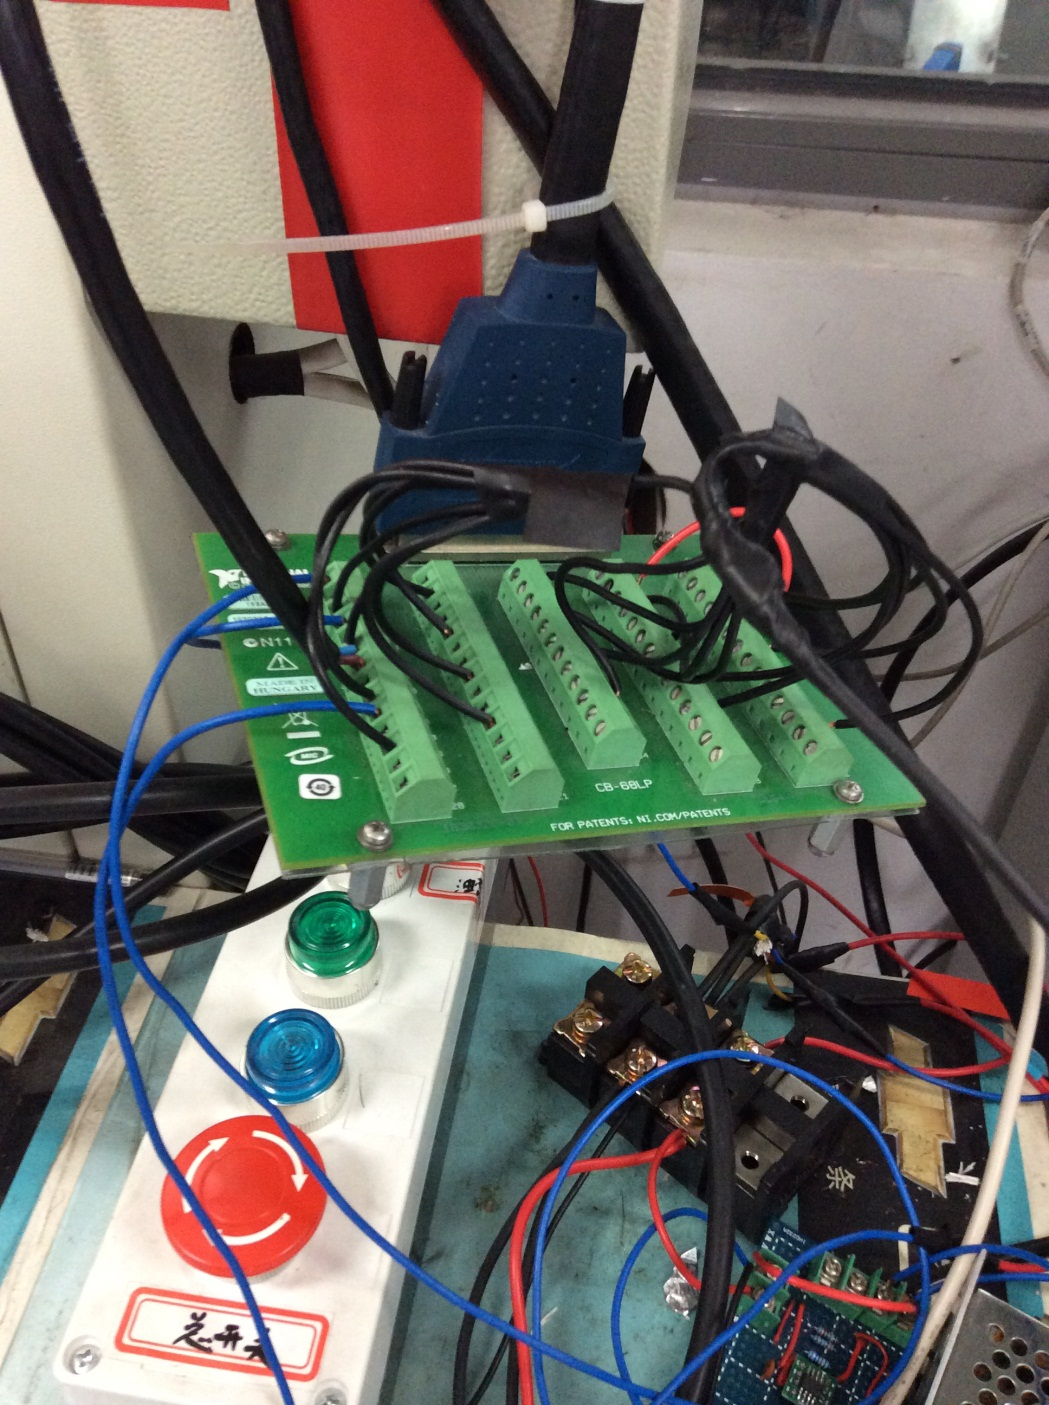
\includegraphics[width=0.4\textwidth]{thesis_figure/platformer_chapter/nicjk}
	\caption{NI��˾�ṩ�IJɼ���}
	\label{fig:nicjk}
\end{figure}
\subsection{�ɼ�����}
�ɼ���������Labview����д����Ҫ��Ϊ�ֶ��ɼ��ʹ����ɼ��������ͣ���ͨ����¼ģʽ�����л��������ֶ��ɼ�ģʽͨ���������ʼ���������ݲ�
�����������ɼ��������ô����������������õ��Ǹ�ѹֵ$>$��ֵ���ɼ�����Ὣ�����÷�ֵ��ǰ��һ��ʱ������ݲɼ�������ͼ\ref{fig:cjcxjm}�Dzɼ�����Ľ��档
\begin{figure}[!ht]
	\centering
	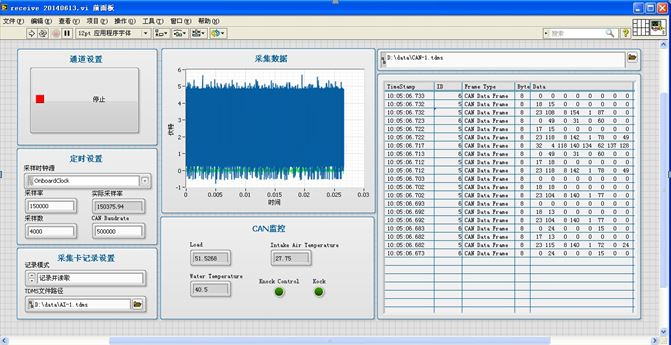
\includegraphics[width=0.9\textwidth]{thesis_figure/platformer_chapter/cjcxjm}
	\caption{�ɼ��������}
	\label{fig:cjcxjm}
\end{figure}
\par�òɼ�������Ҫ�ɶ�ʱ���ã��ɼ�����¼���ã�CAN��أ�����ʵʱ��ʾ��ͨ�����ؼ���������ɡ���ʱ���ÿ������ò���ʱ�ӡ��������������ʵȹؼ��������ɼ�����¼����
���������ļ������·����CAN��ؿ���ʵʱ���ɼ������Ƿ����쳣��ͬʱҲ����ͨ������ʵʱ��ʾ���������鿴���ݲɼ������Ƿ����쳣��






\chapter{离子电流干扰去除分析方法}
\section{电容式离子电流检测电路的局限性}
\par如下图所示的是1250r/min,2000r/min,3000r/min下在30\%,40\%,50\%时的缸压和离子电流曲线。
\begin{figure}[H]
	\centering
	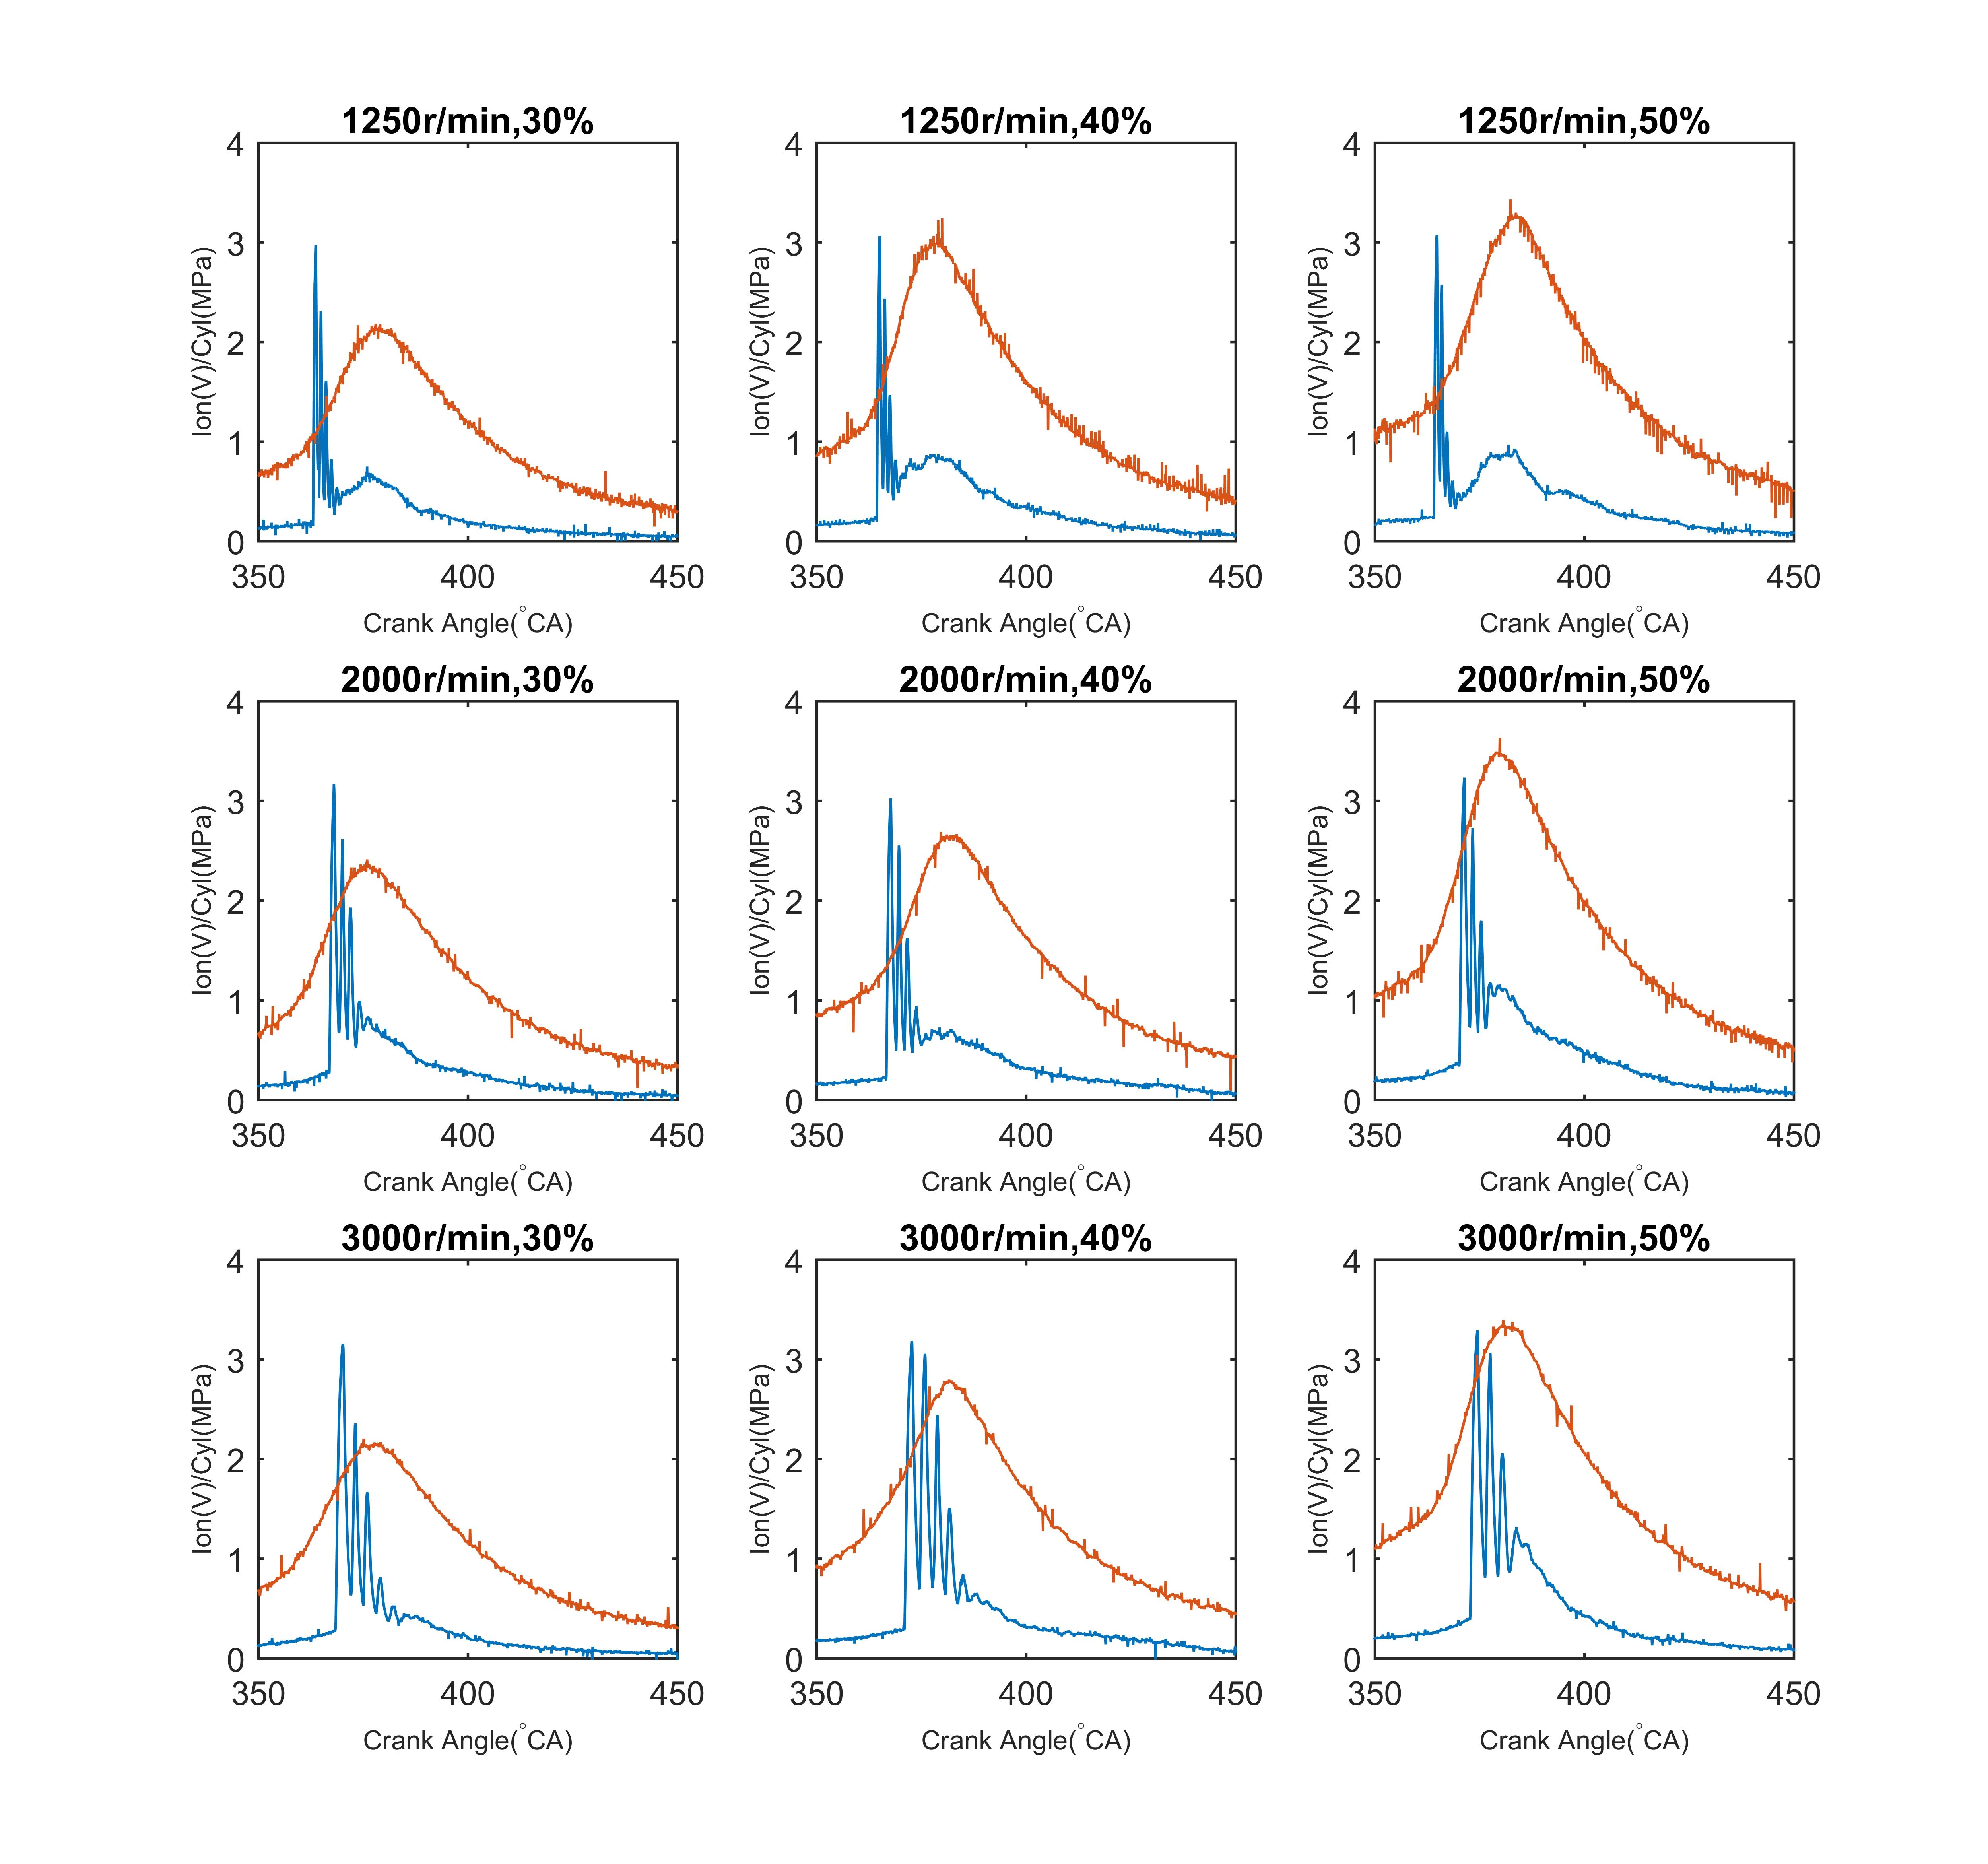
\includegraphics[width=\textwidth]{thesis_figure/ion_chapter/ion_vary_trending}
	\caption{不同转速、不同负荷下的缸压和离子电流}
	\label{fig:ion_cyp}
\end{figure}
从图\ref{fig:ion_cyp}中可以看到从上到下看是同一负荷下,随着转速增加的离子电流曲线;从左向右是同一转速下,随着负荷增大的离子电流曲线。
随着转速的增加,火焰后期的离子电流是逐渐被淹没的。也就是说点火干扰期将离子电流的性质淹没了,无法获得离子电流的特征值。
\subsection{点火放电干扰的来源和性质}
由于点火干扰期将离子电流的性质淹没,因此我们需要了解点火放电干扰的来源及其稳定的性质。如图\ref{fig:itf_rs}所示,通过检测次级电压来和离子电流进行对比可以发现,次级电压
点火放电过程的放电干扰期和离子电流的点火干扰期重合。
\begin{figure}[H]
\begin{minipage}{0.5\linewidth}
	\centering
	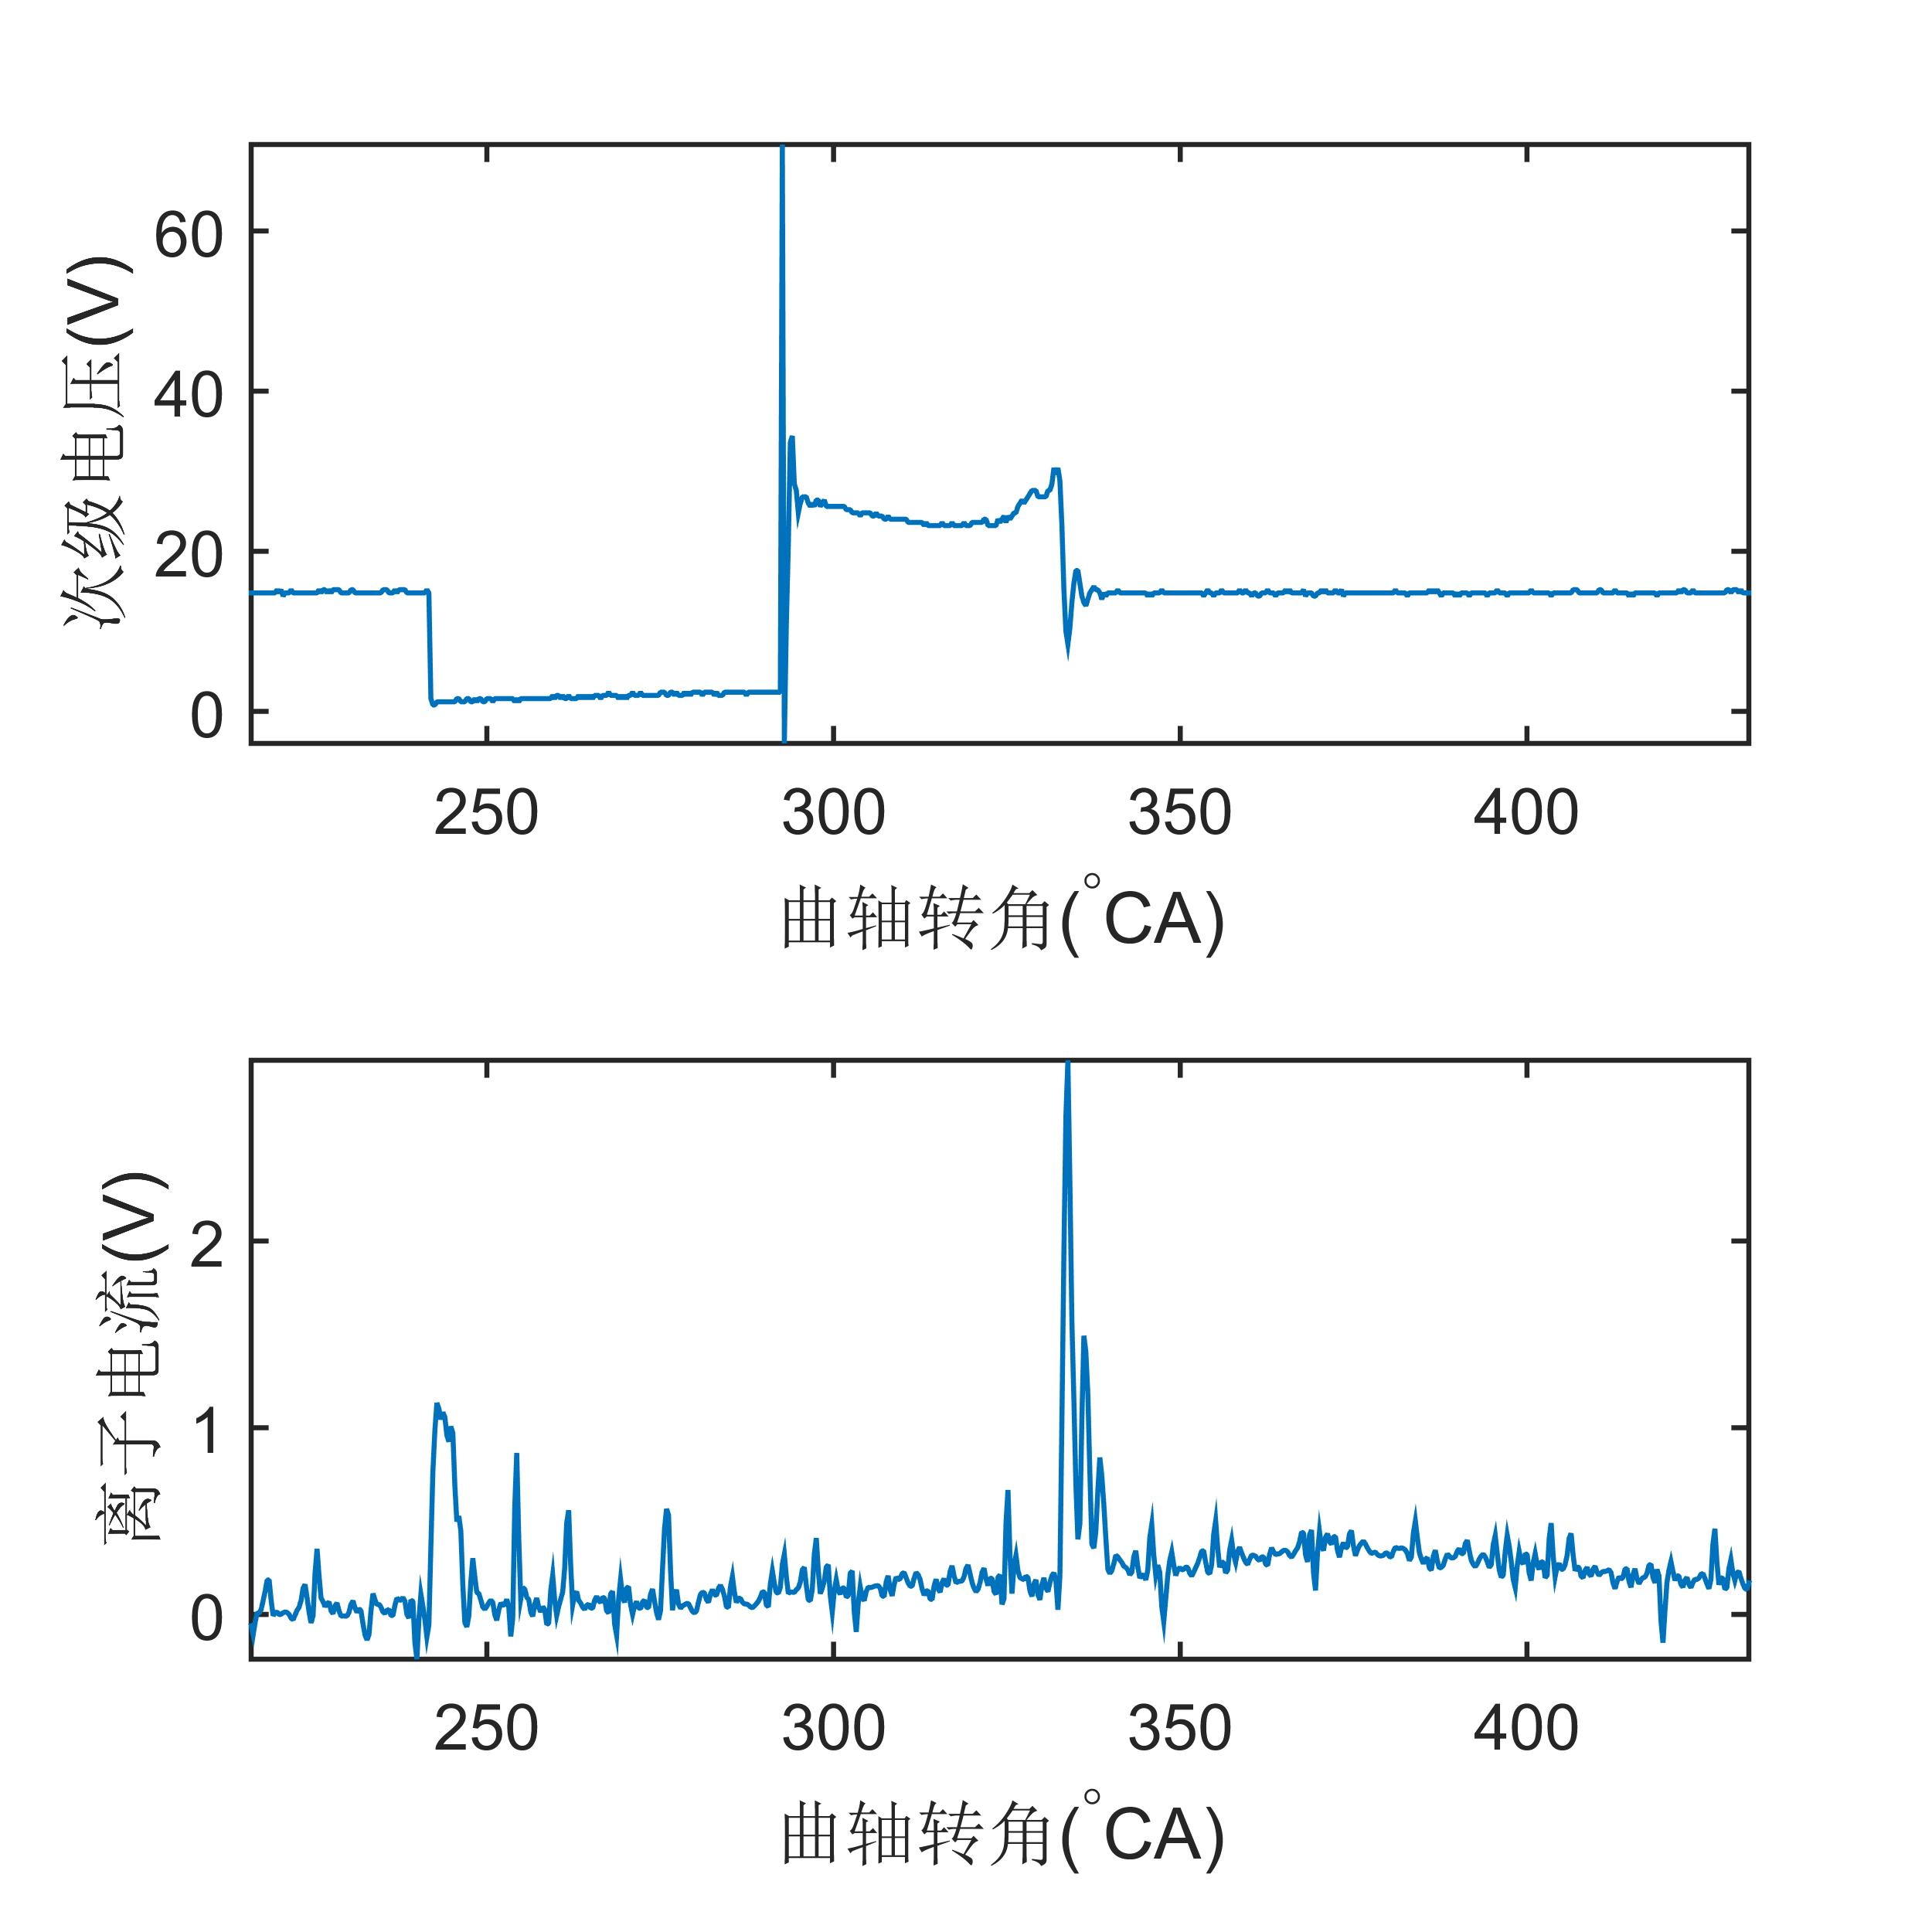
\includegraphics[width = \textwidth]{thesis_figure/ion_chapter/interfere_reason}
\end{minipage}
\begin{minipage}{0.5\linewidth}
	\centering
	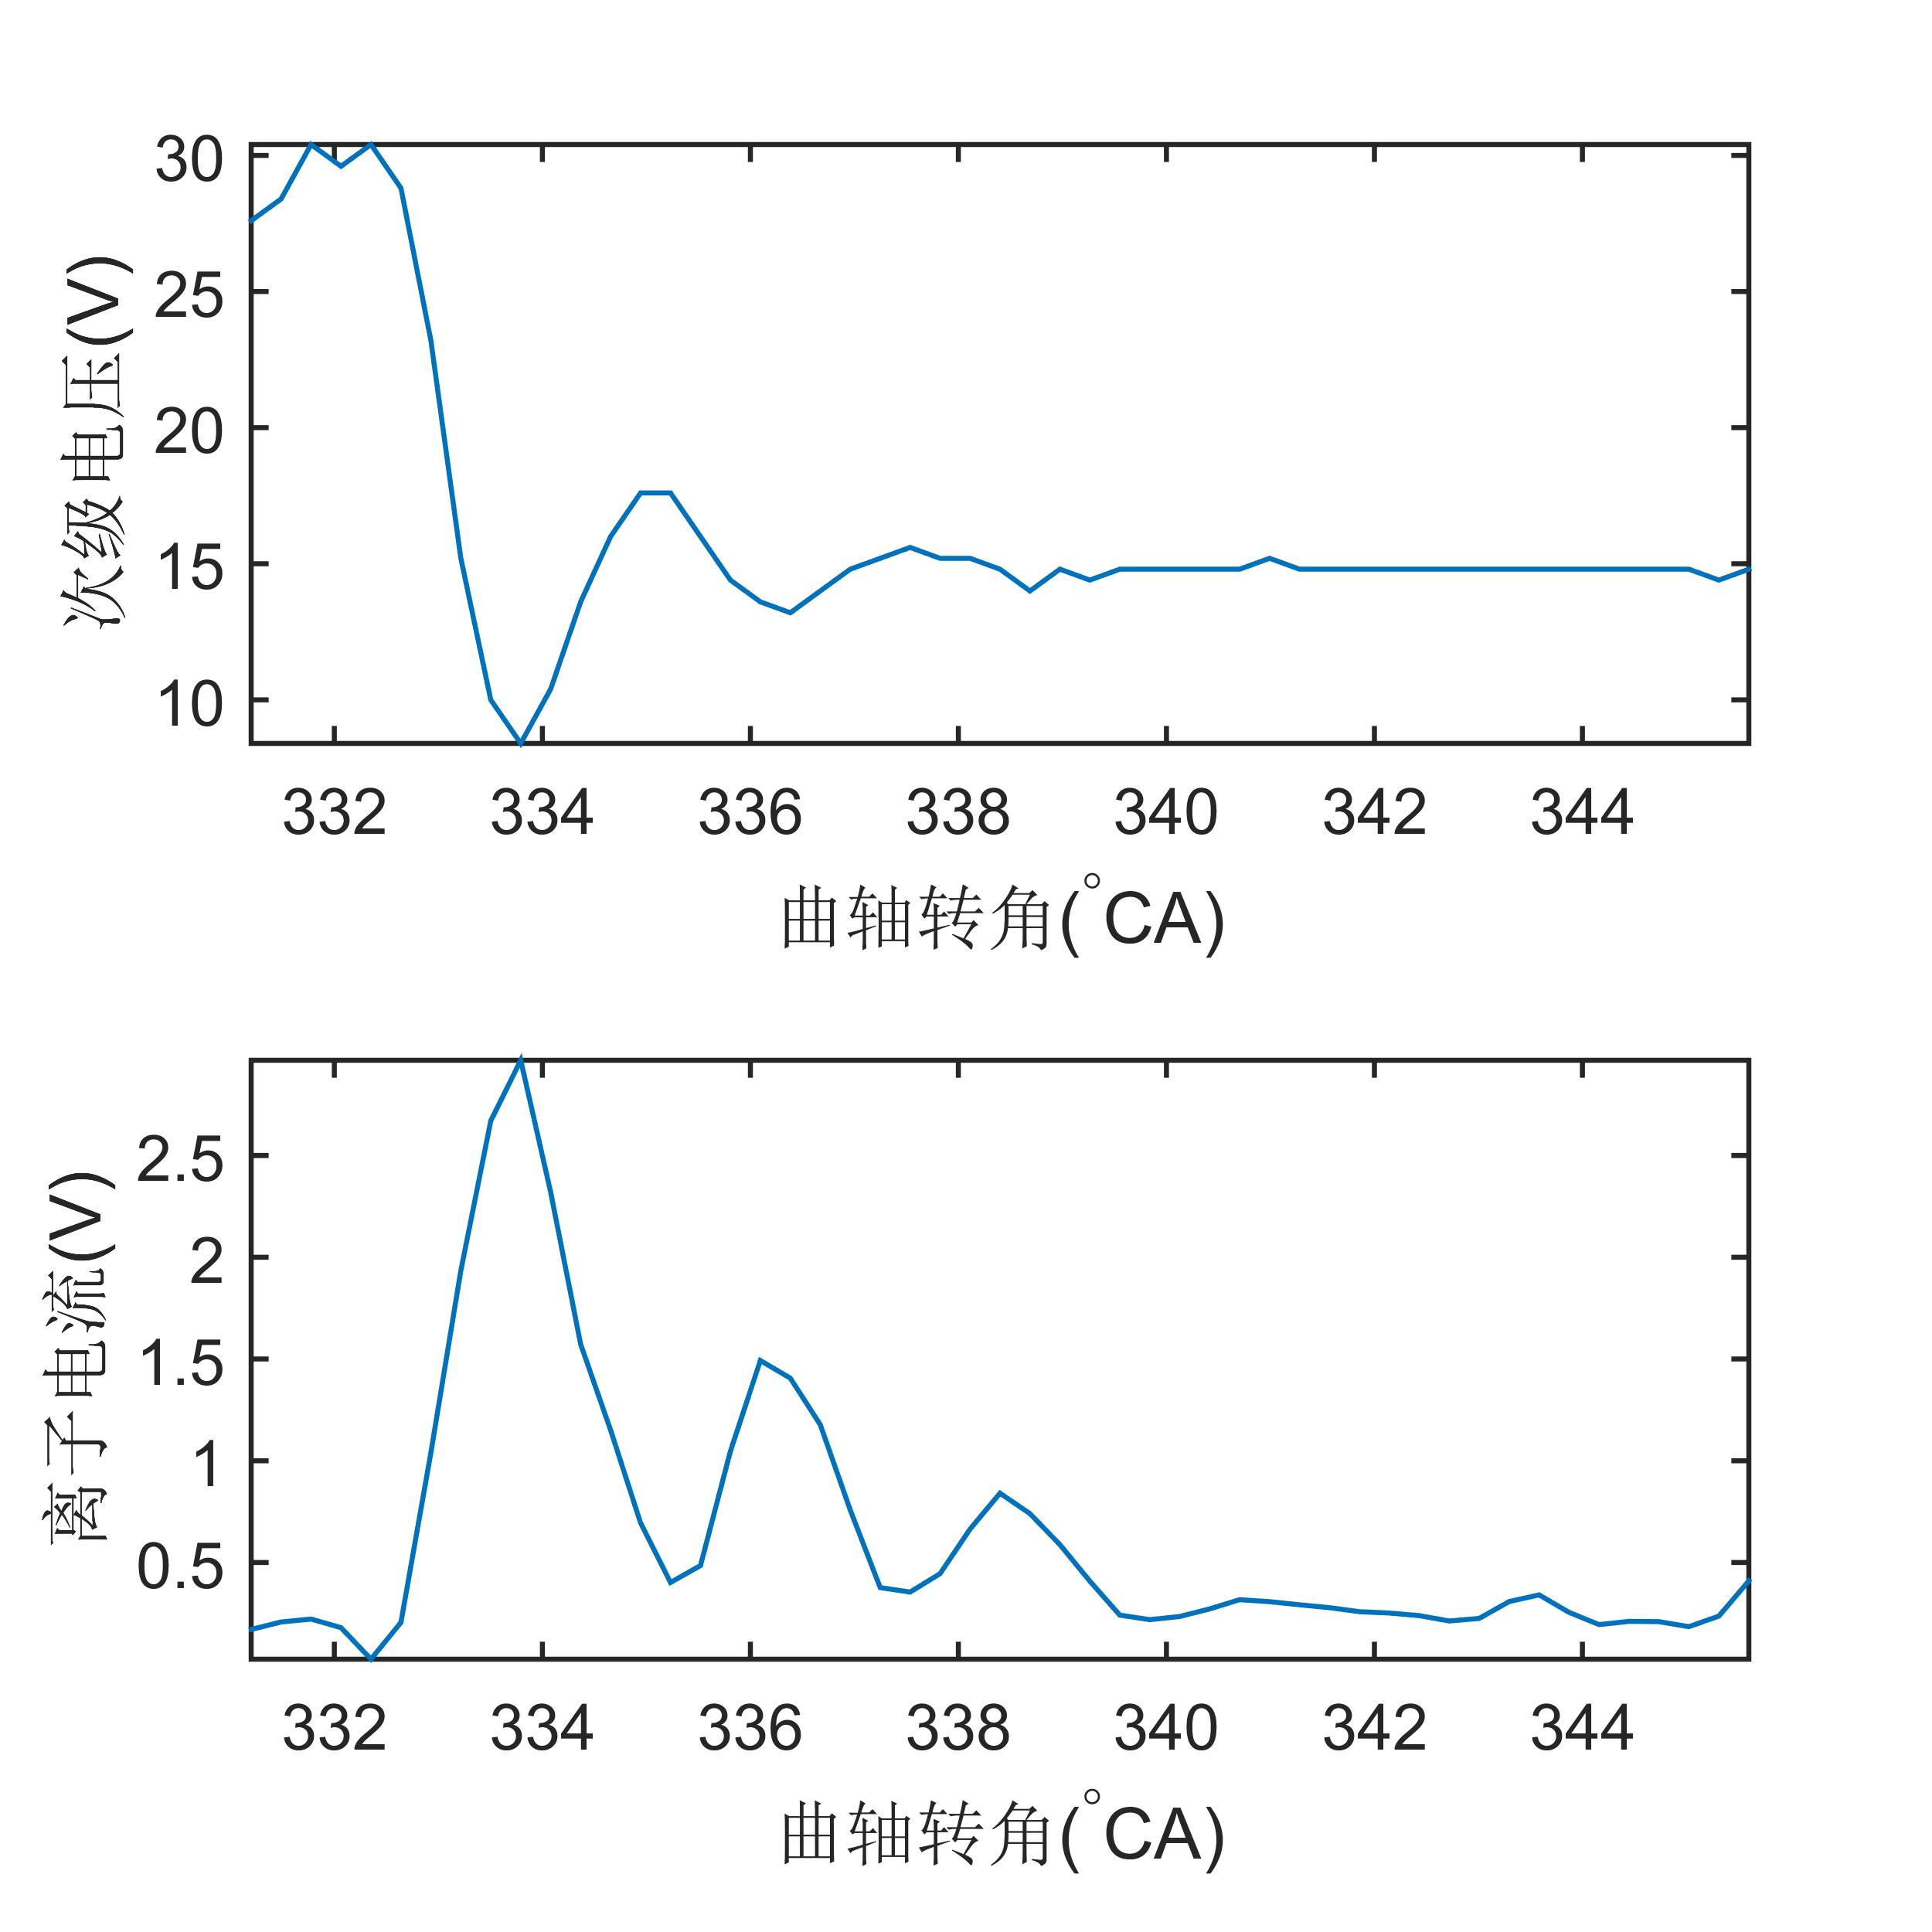
\includegraphics[width = \textwidth]{thesis_figure/ion_chapter/itf_rs}
\end{minipage}
	\caption{次级电压和离子电流对比}
	\label{fig:itf_rs}
\end{figure}
\par我们将重叠的部分进行放大,可以看到两者的频率也是相同的。
经过计算可以得到该放电周期为$0.12ms$,时长为$1ms$。由以上两张图的分析结果可以知道,离子电流的点火干扰期是由次级线圈的点火放电信号导致的,会产生一个特定频率的震荡信号。我们将不同转速下的离子电流
曲线放在一起比较,可以看到如图\ref{fig:dif_rpm_ion}所示的图形。
\begin{figure}[!ht]
	\centering
	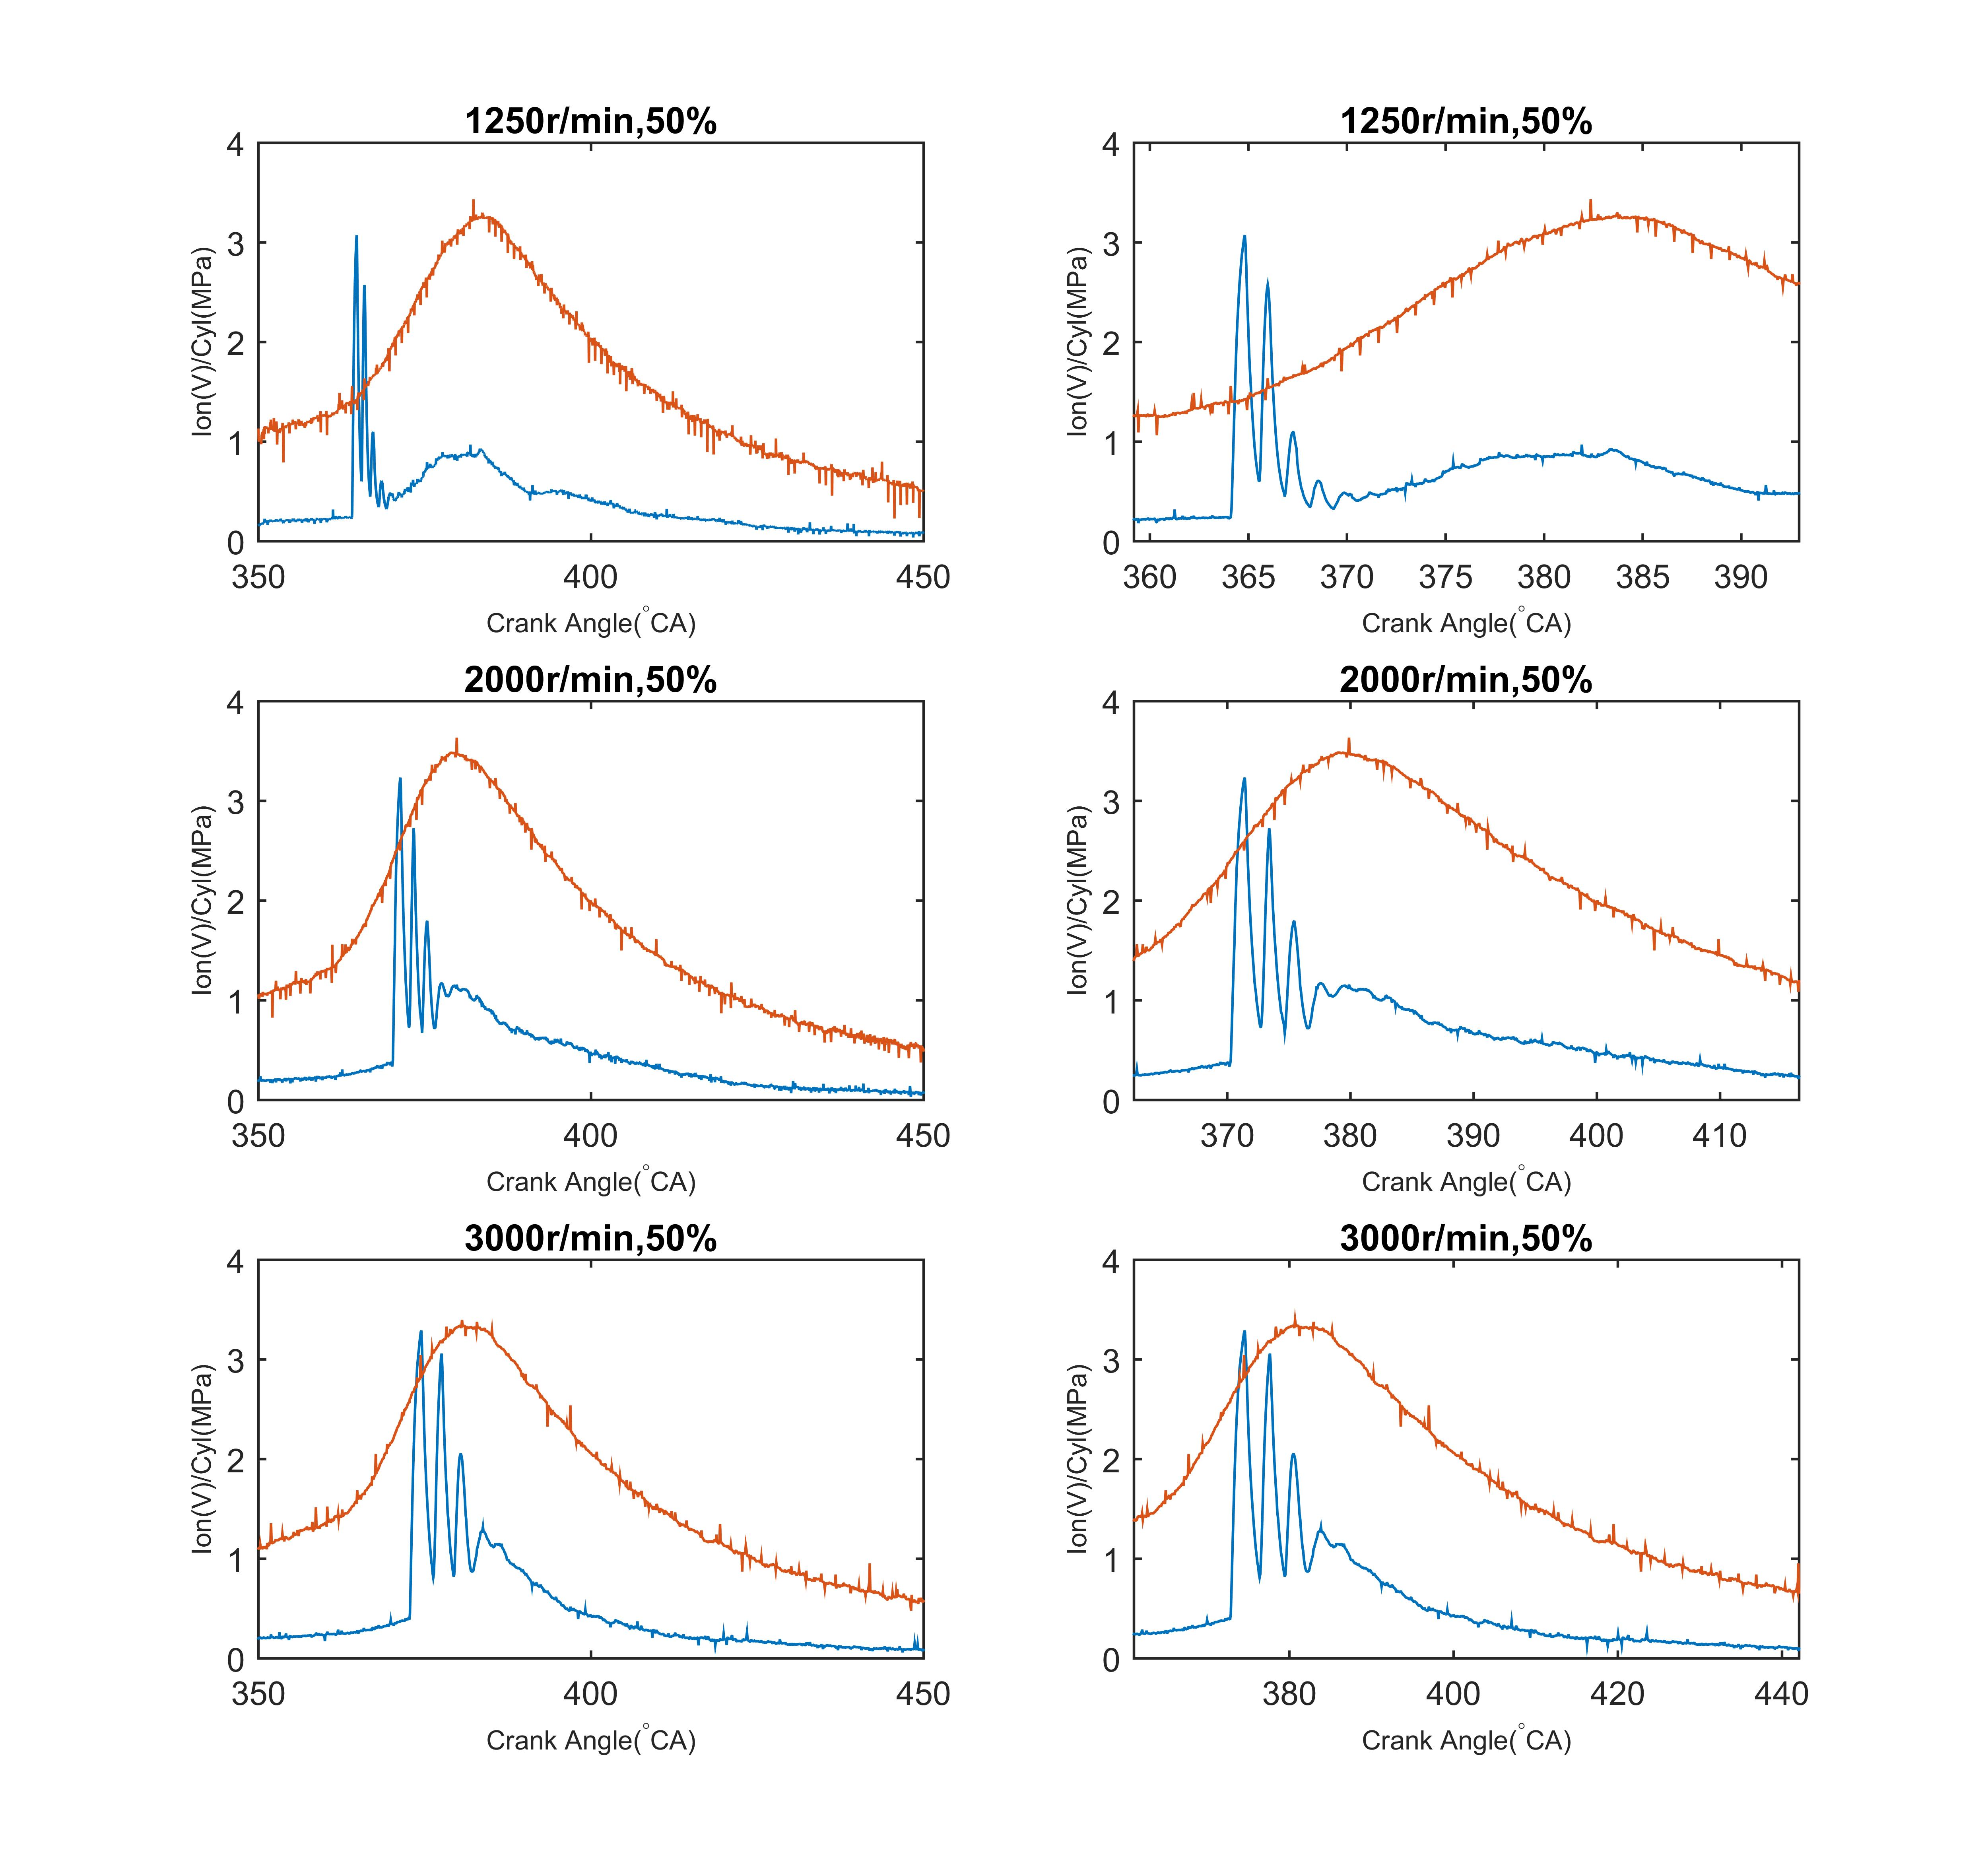
\includegraphics[width=\textwidth]{thesis_figure/ion_chapter/dif_rpm_ion}
	\caption{不同转速下的离子电流按曲轴转角对比和按时间对比}
	\label{fig:dif_rpm_ion}
\end{figure}
\par左列的三张图从上到下为随着转速增加,离子电流按照曲轴转角进行对比,曲轴转角窗口长度为100度,可以发现点火震荡信号在不断淹没火焰前锋期和火焰后期。右列的三张图从上到下为随着转速增加,
离子电流按时间进行对比,时间窗口长度为5毫秒时间,可以发现震荡信号的频率和长度不变。左右两列曲线分别对应了该工况下的同一个循环,由此可以知道该震荡信号具有稳定的时间长度,稳定的频率特性。
%\par这一部分需要有一个电路仿真过程来支撑。获得$R_g$的电流曲线形状,该形状肯定是没有震荡过程的。
%分析用于支持后面的两个算法是正确的,确定点火干扰期的信号形状。离子电流肯定是频率较低的信号,所以需要去除掉信号中的高频
%信号。
%\par有个很重要的现象。随着转速的增加,火焰后期的离子电流的升高速率也会较快,从而和火焰前期的离子电流有重合迹象。
\subsection{断油情况下的点火干扰分析}
当发动机断油情况下,点火线圈仍然进行点火过程,但是缸内由于没有燃气,无法形成化学电离过程的离子电流信号,所以断油情况下的点火干扰具有稳定而且清晰的特征。如图\ref{fig:dy_ion}所示是一个断油情况下的电容
式检测电路检测到的电压曲线。
\par从图中可以看到缸压曲线峰值相位在上止点360度位置,说明该循环处于纯压缩循环。可以看到此时的离子电流信号的峰值位置也是上止点位置,此时的离子电流信号是热电离导致的,没有化学电离产生的离子电流信号。
\begin{figure}[H]
\begin{minipage}[t]{0.5\linewidth}
	\centering
	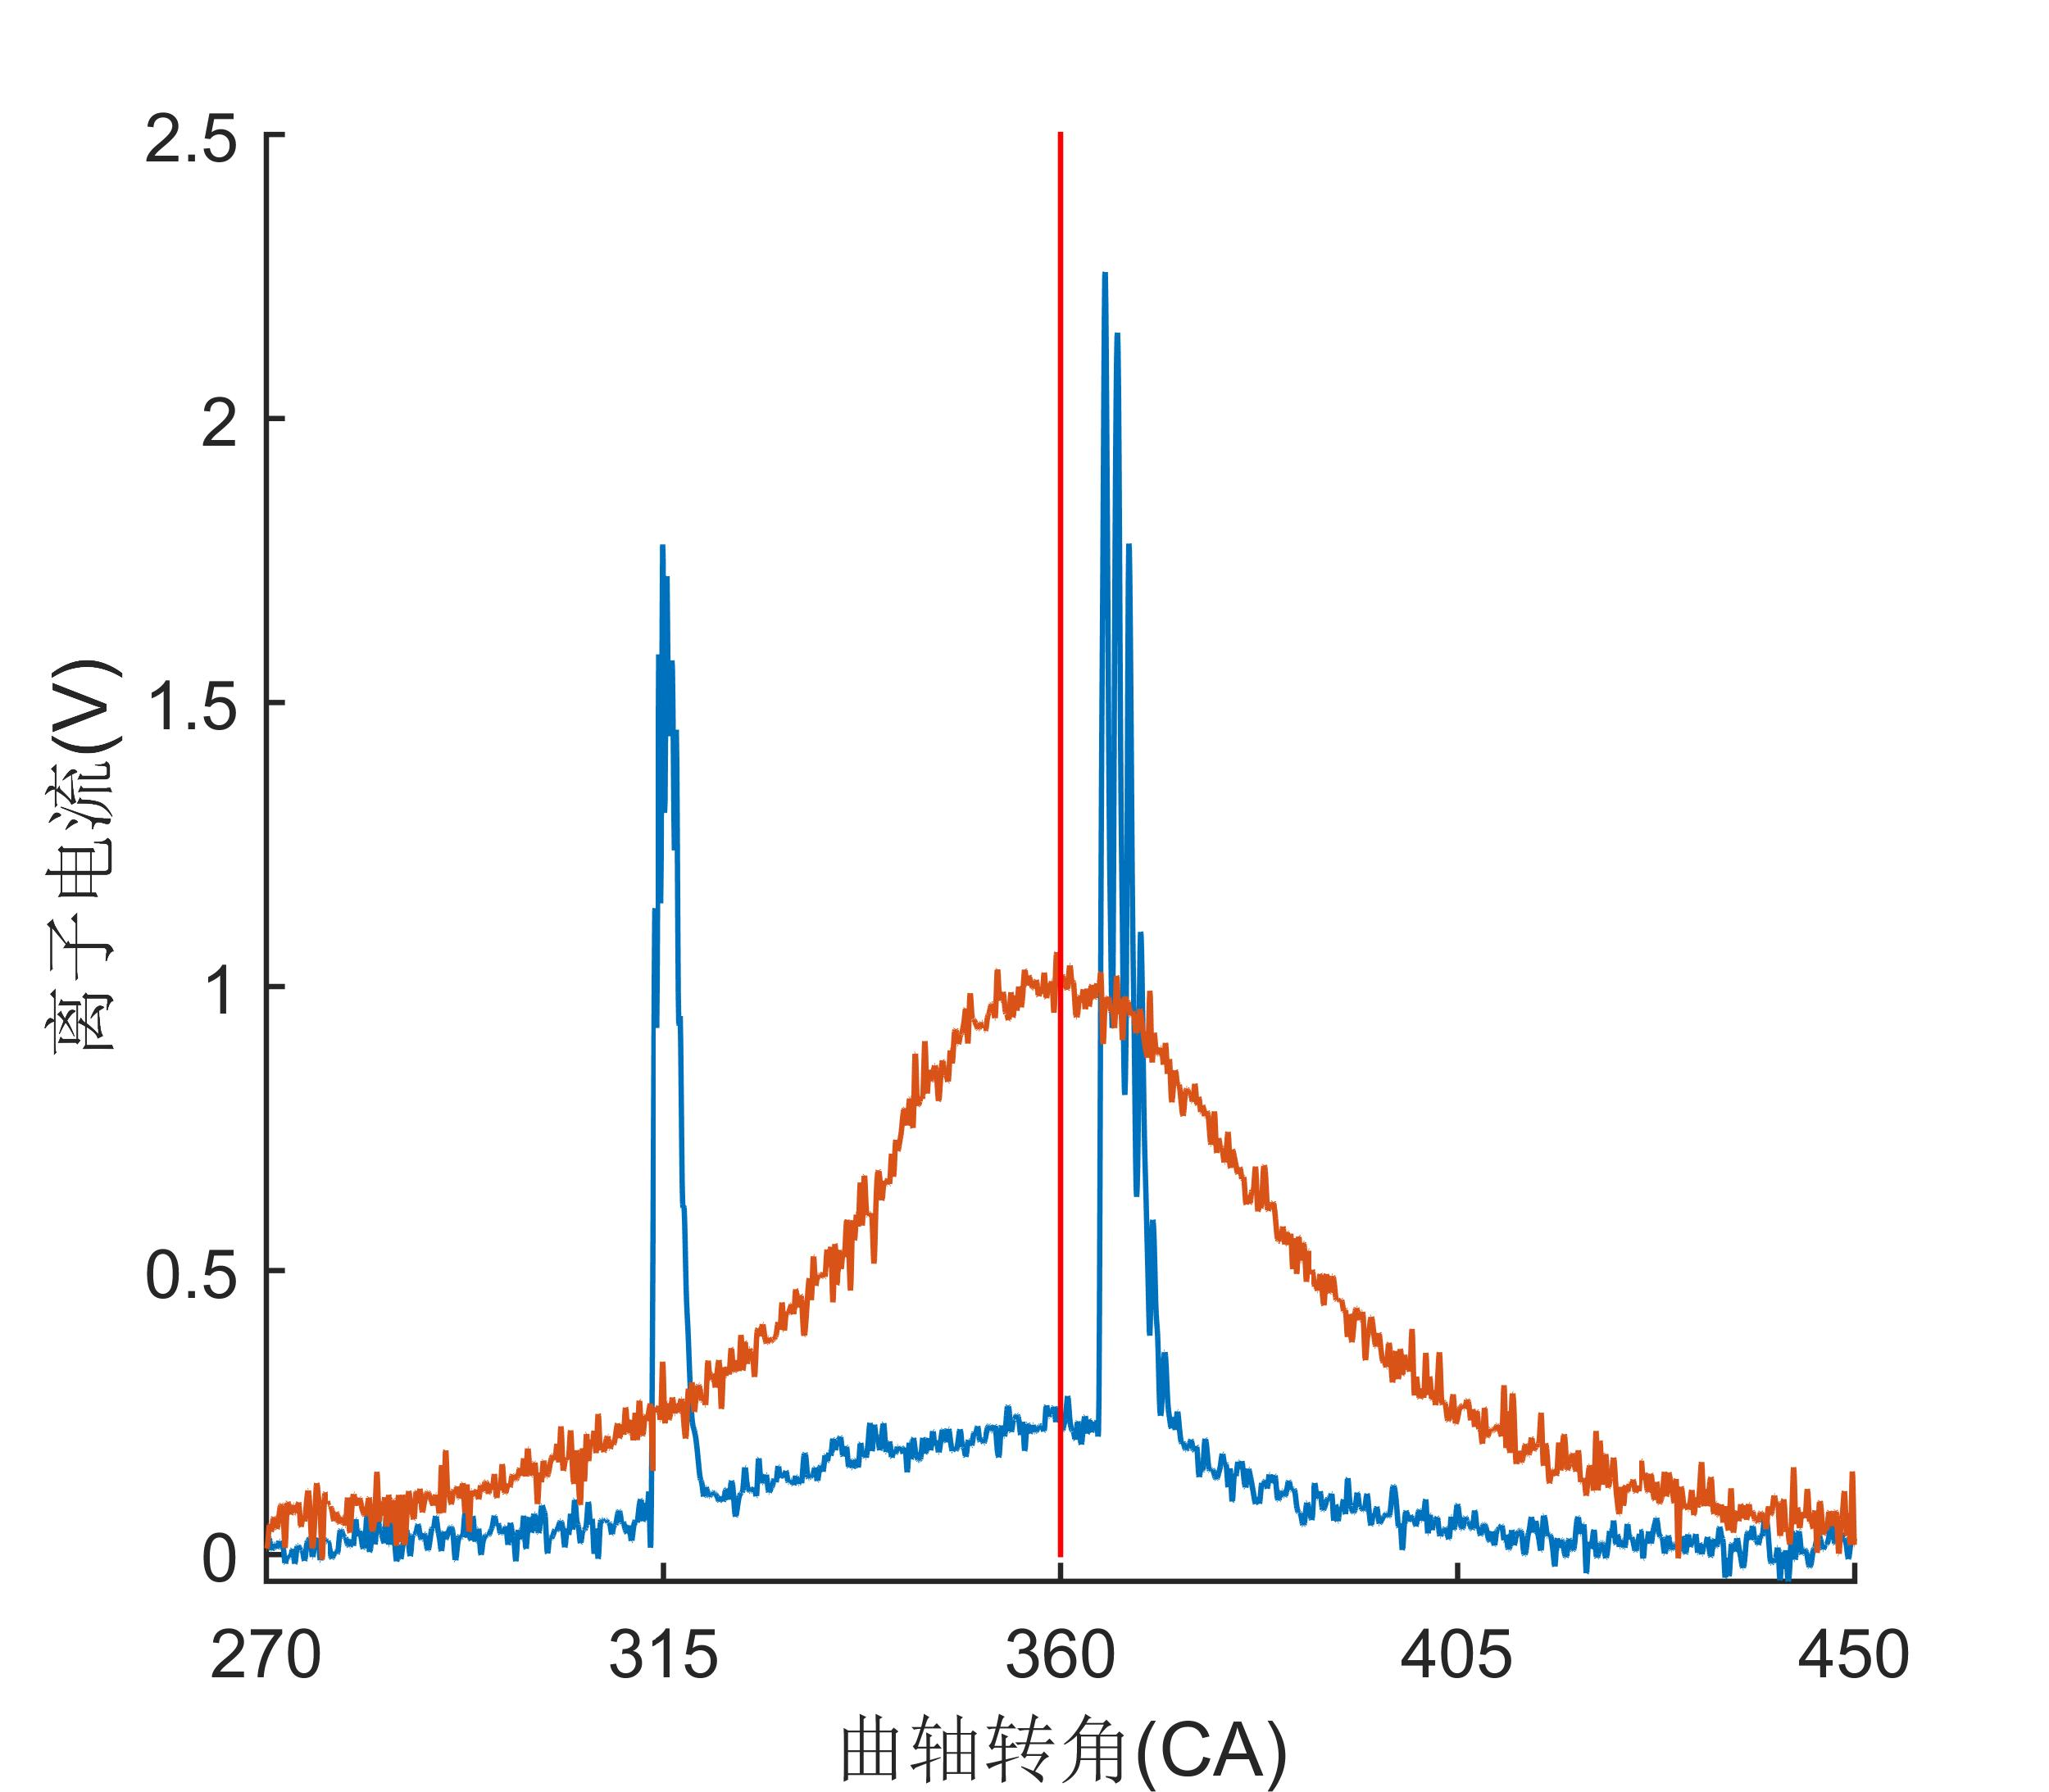
\includegraphics[width=\textwidth]{thesis_figure/ion_chapter/dy_ion}
	\caption{断油情况下的电压信号}
	\label{fig:dy_ion}
\end{minipage}
\begin{minipage}[t]{0.5\linewidth}
	\centering
	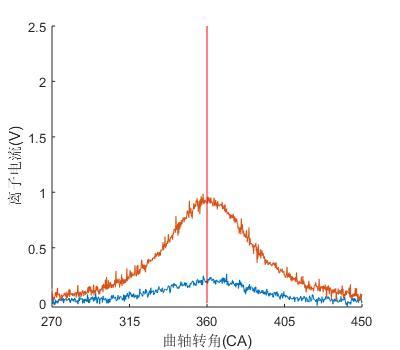
\includegraphics[width=\textwidth]{thesis_figure/ion_chapter/dh_ion}
	\caption{断火情况下的电压信号}
	\label{fig:dh_ion}
\end{minipage}
\end{figure}
\subsection{断火情况下的离子电流分析}   
当发动机断火情况下,点火线圈不进行点火过程,导致缸内混合气不能进行燃烧过程,无法形成化学电离过程的离子电流信号如图\ref{fig:dh_ion}所示是一个断火情况下的电容式检测电路检测到的电压信号。
\par从图\ref{fig:dh_ion}中可以看到缸压曲线峰值相位在上止点360度位置,说明该循环处于纯压缩循环。可以看到此时的离子电流信号的峰值相位也是上止点位置,此时的离子电流信号是热电离导致的,没有化学电离产生的离子电流信号。
\subsection{纯点火干扰的分析方法}
对比图\ref{fig:dy_ion}和图\ref{fig:dh_ion},可以看到无论断油还是断火,都会导致缸内的混合气体无法燃烧,不能够产生化学电离,两者的循环都是纯压缩循环。
同时热电离曲线的形状和峰值大小都类似。所以可以将同一转速和负荷下的离子电流信号相减,即可得到近似的纯点火干扰信号。
\begin{figure}[ht]
\begin{minipage}[t]{0.5\linewidth}
	\centering
	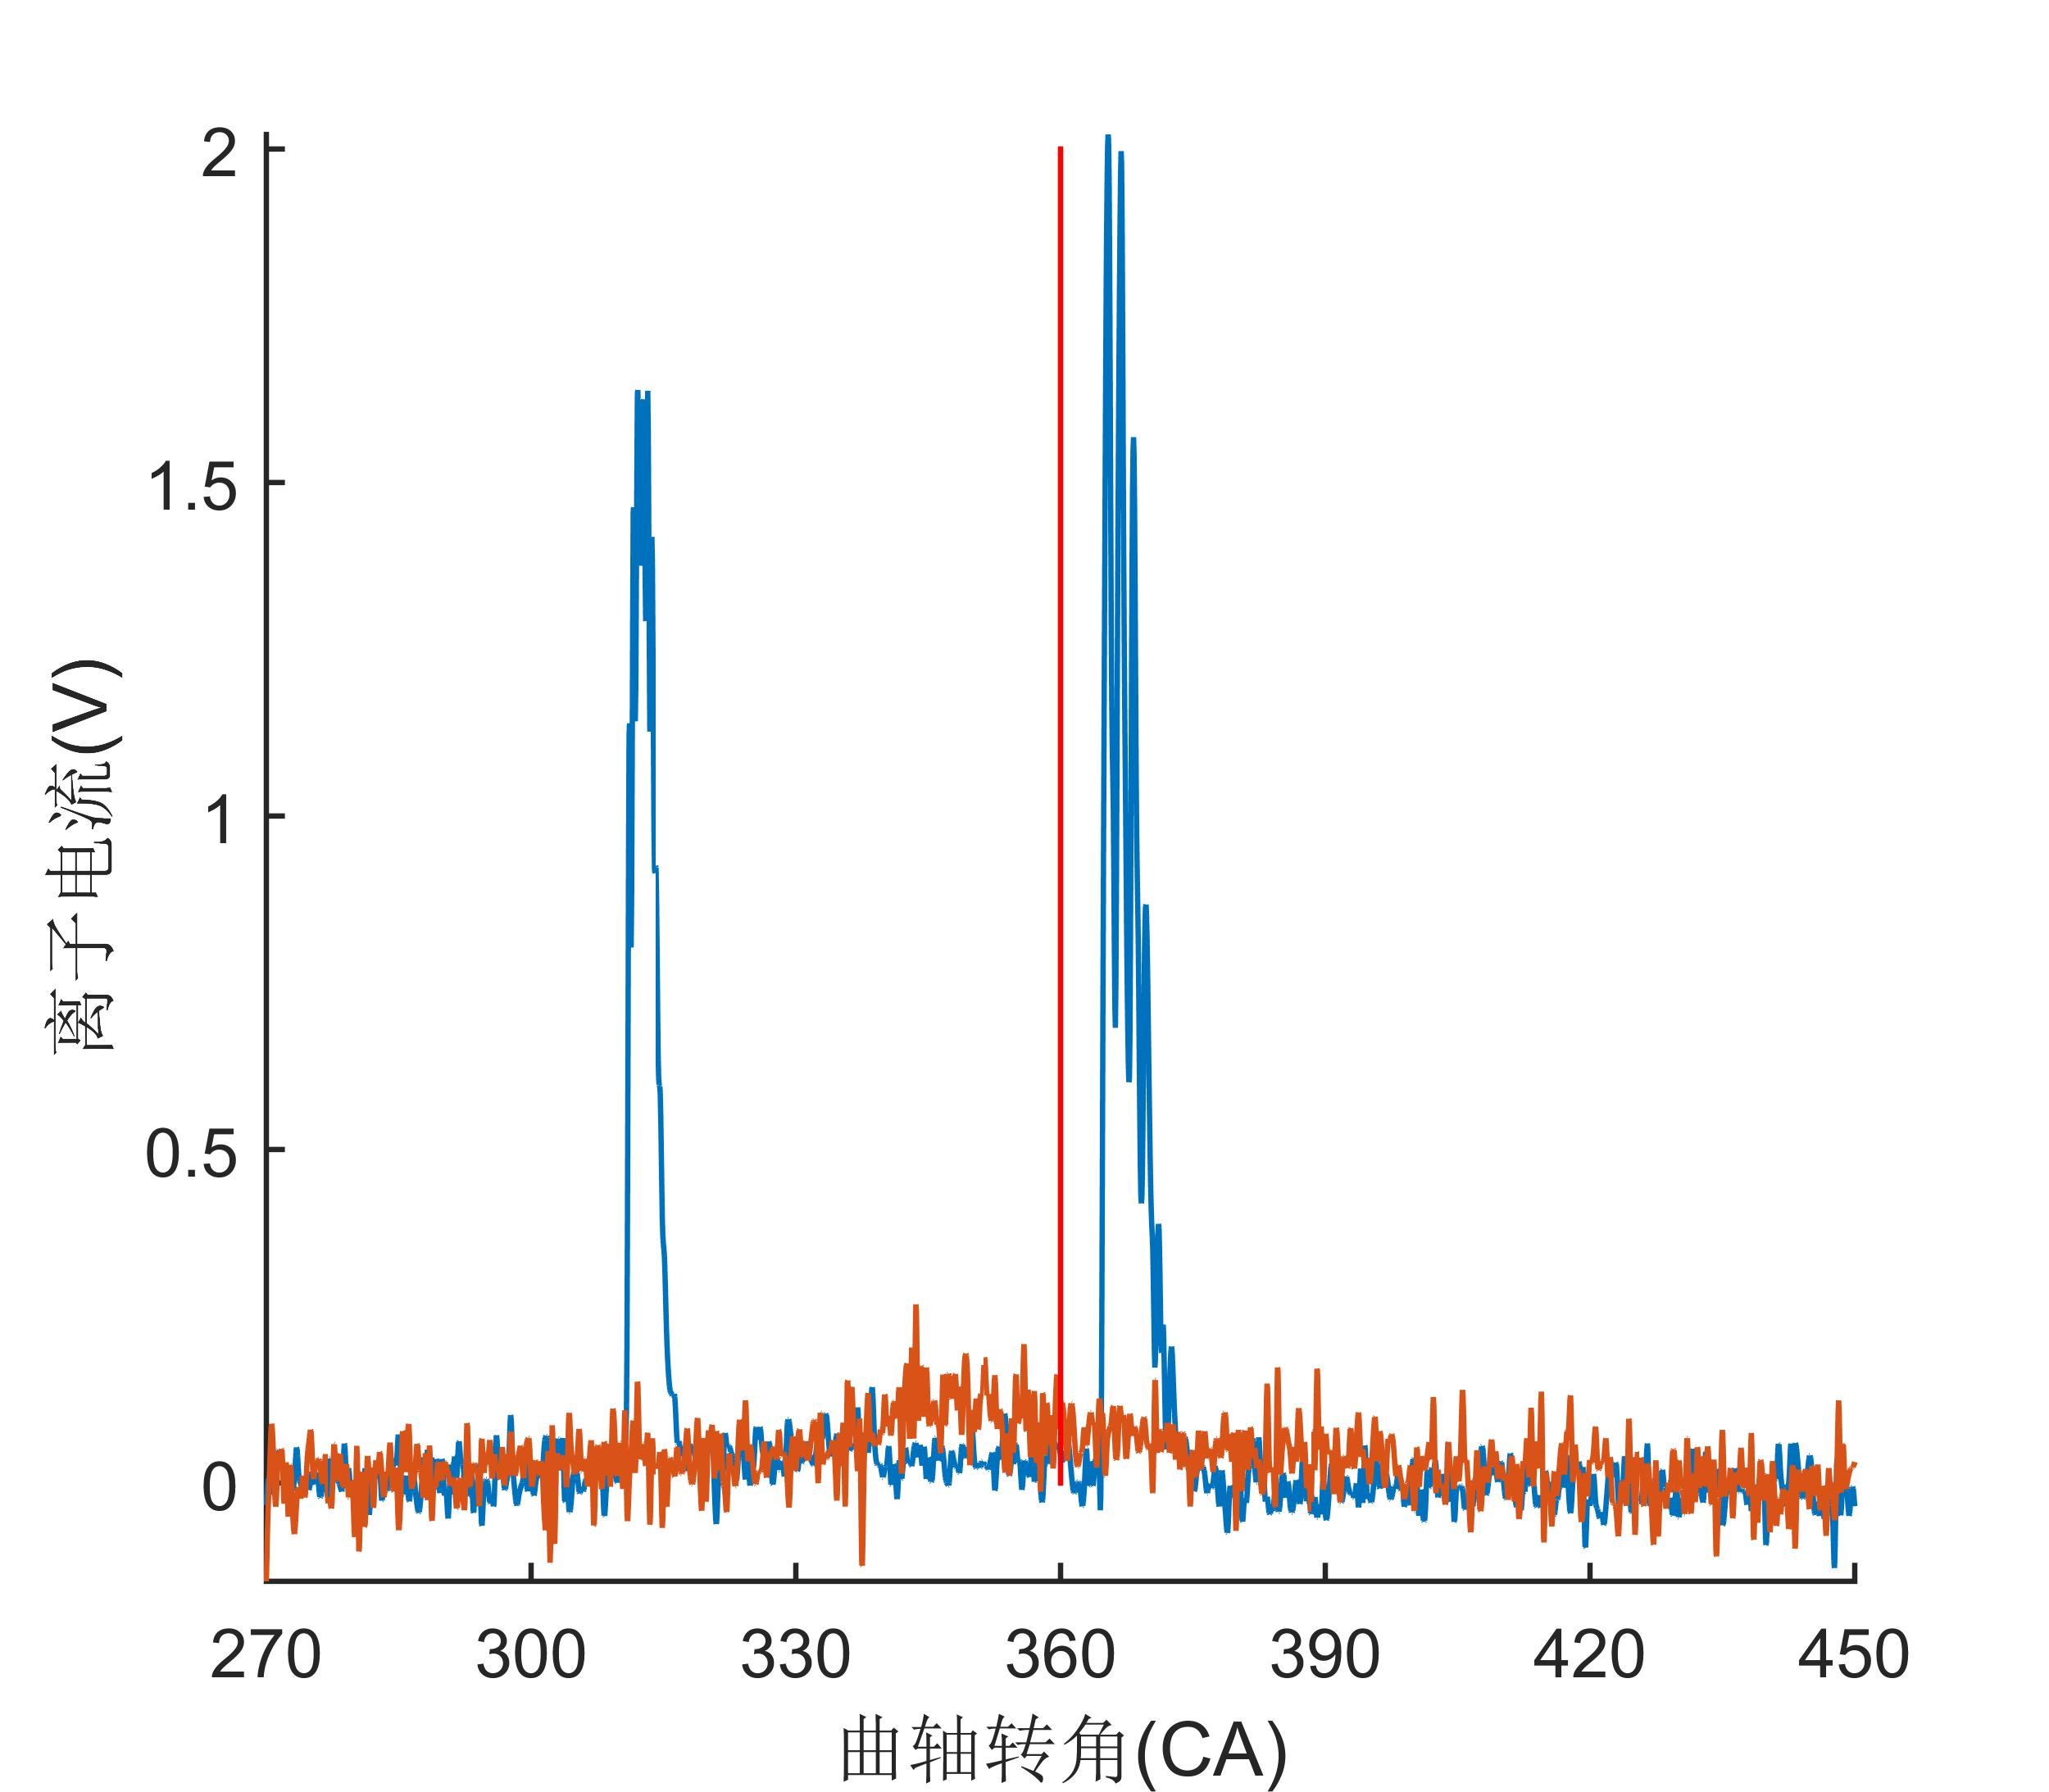
\includegraphics[width=\textwidth]{thesis_figure/ion_chapter/diff_dy_dh}
\end{minipage}
\begin{minipage}[t]{0.5\linewidth}
	\centering
	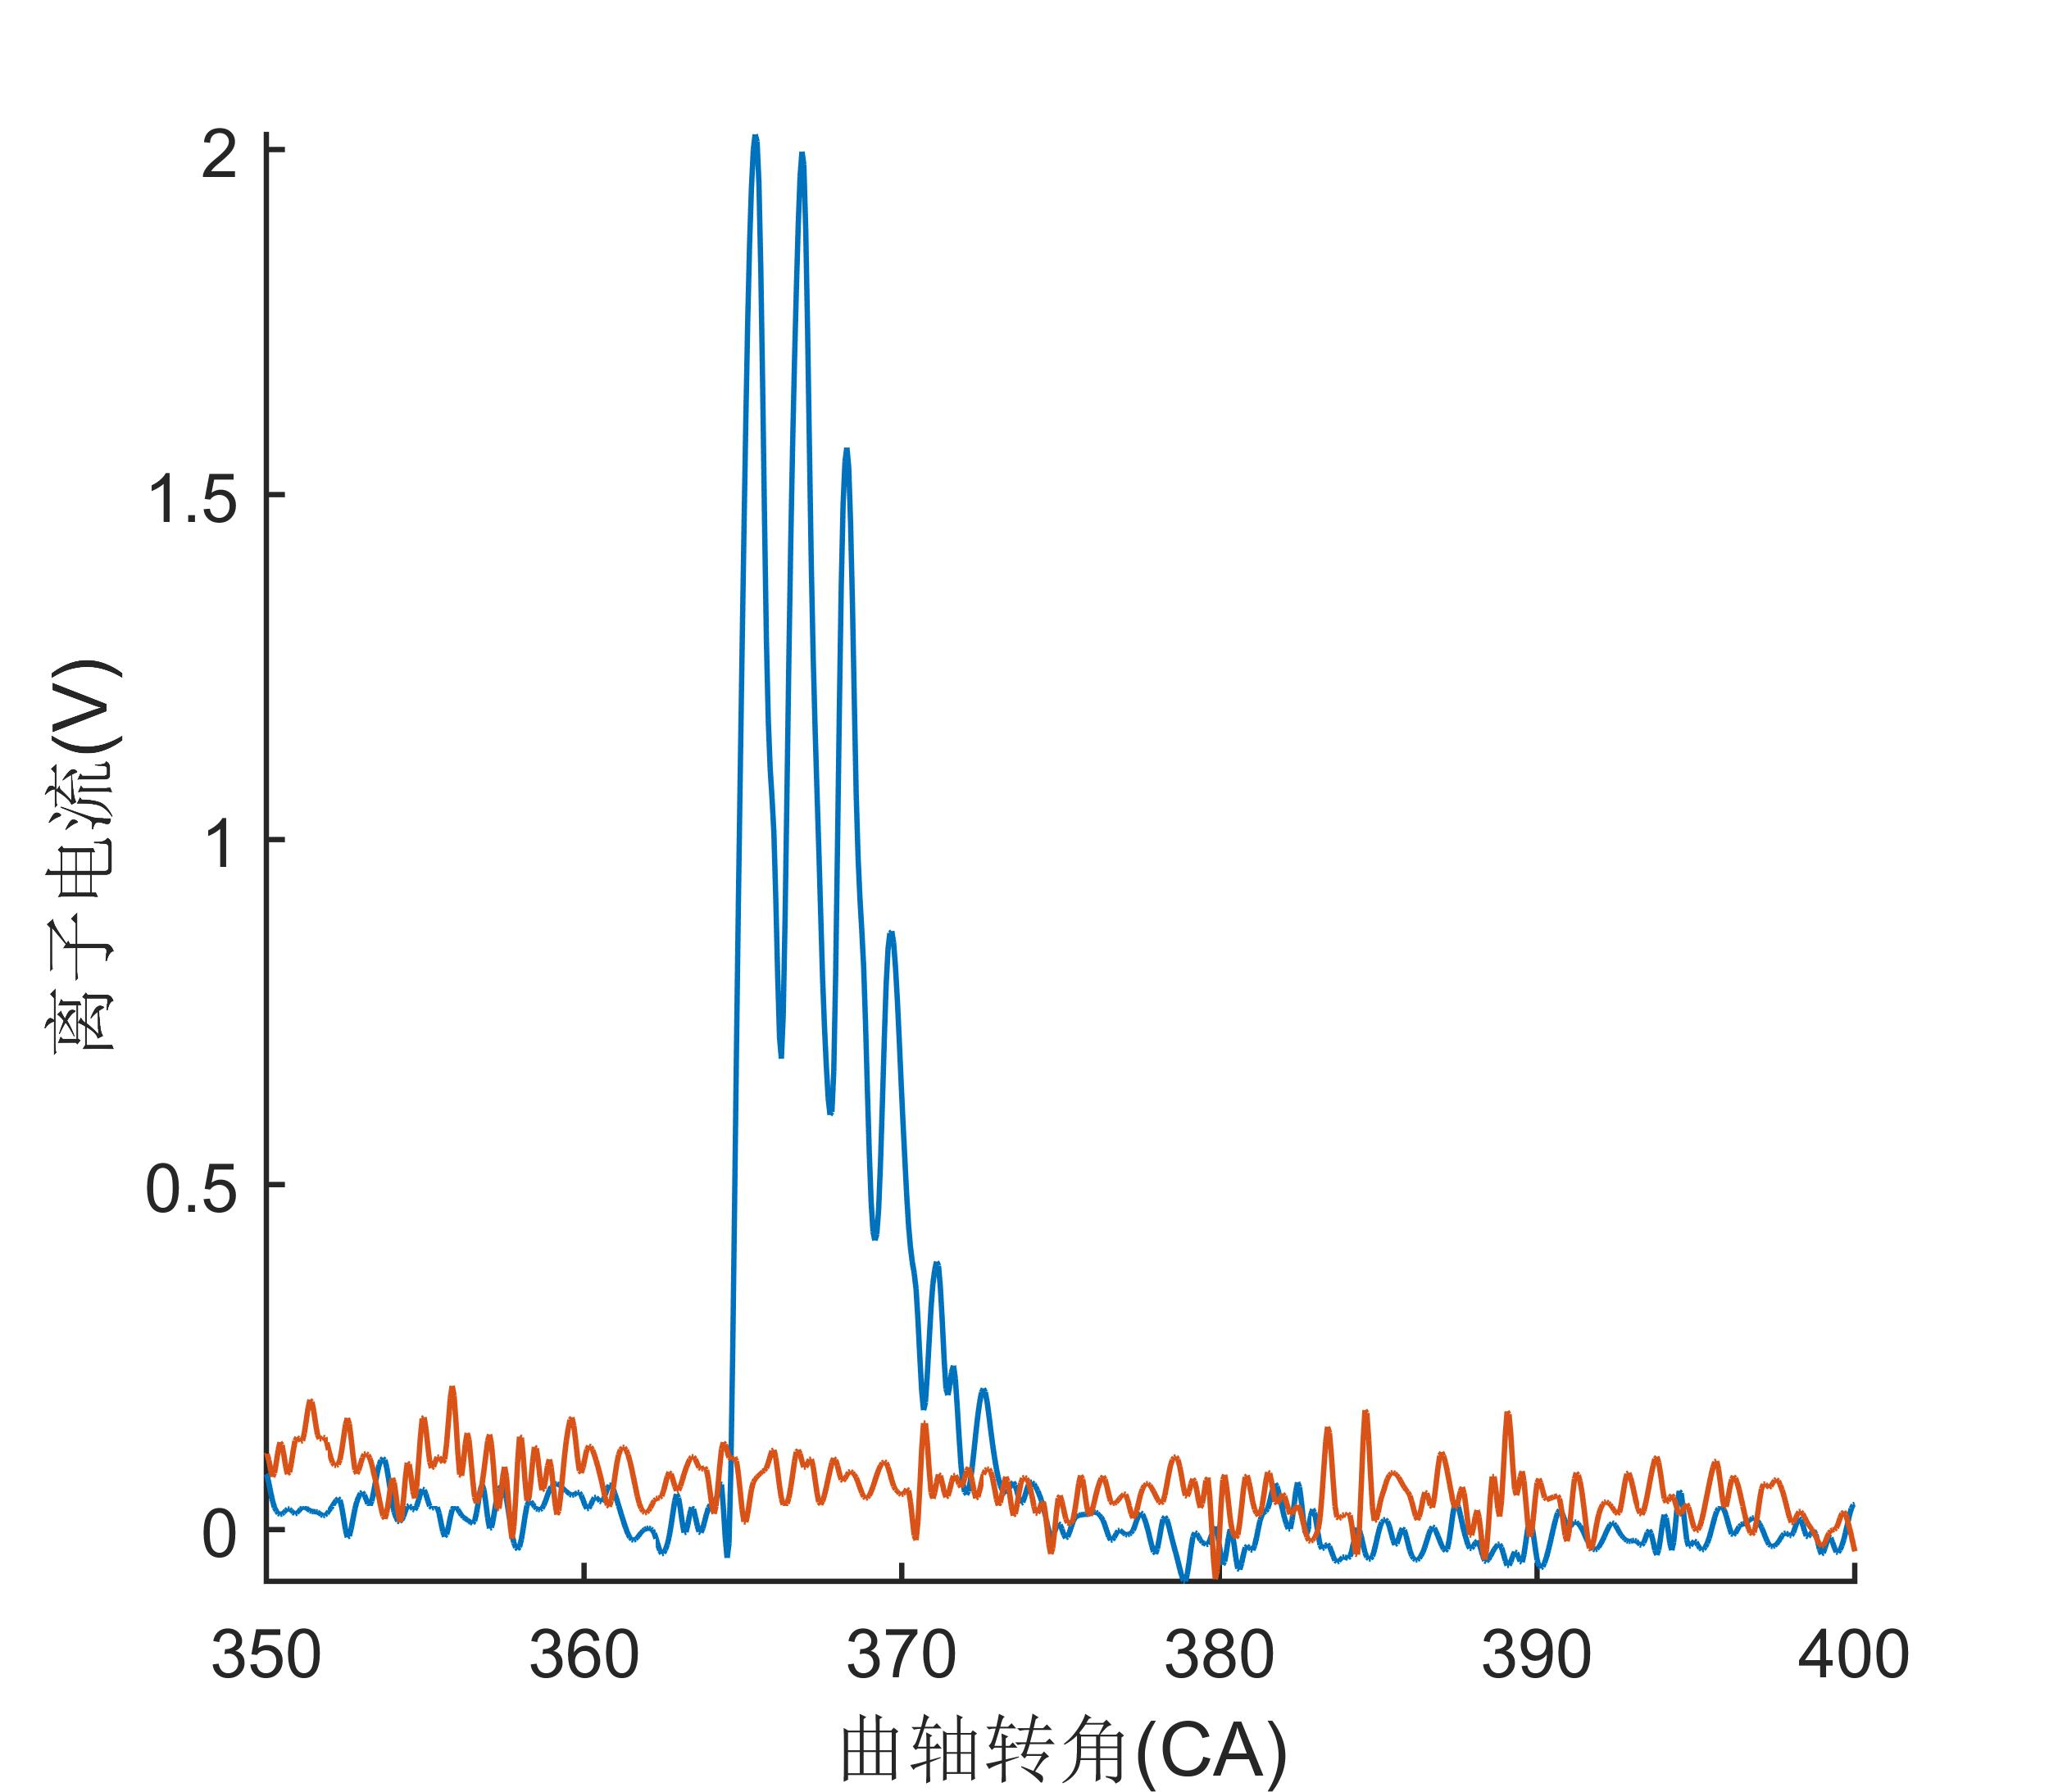
\includegraphics[width=\textwidth]{thesis_figure/ion_chapter/diff_dy_dh_detail}
\end{minipage}
	\caption{断油离子电流信号与断火离子电流信号差值}
	\label{fig:diff_dy_dh}
\end{figure}
如图\ref{fig:diff_dy_dh}所示可以得到近似的纯点火干扰信号。可以看到两者的缸压曲线也是近似的,说明在同一个工况下的断油和断火循环,造成的缸内情况是类似的,因此两者相减得到的离子电流信号在一定
程度上是可以表征纯电火干扰信号的。
\begin{figure}[H]
	\centering
	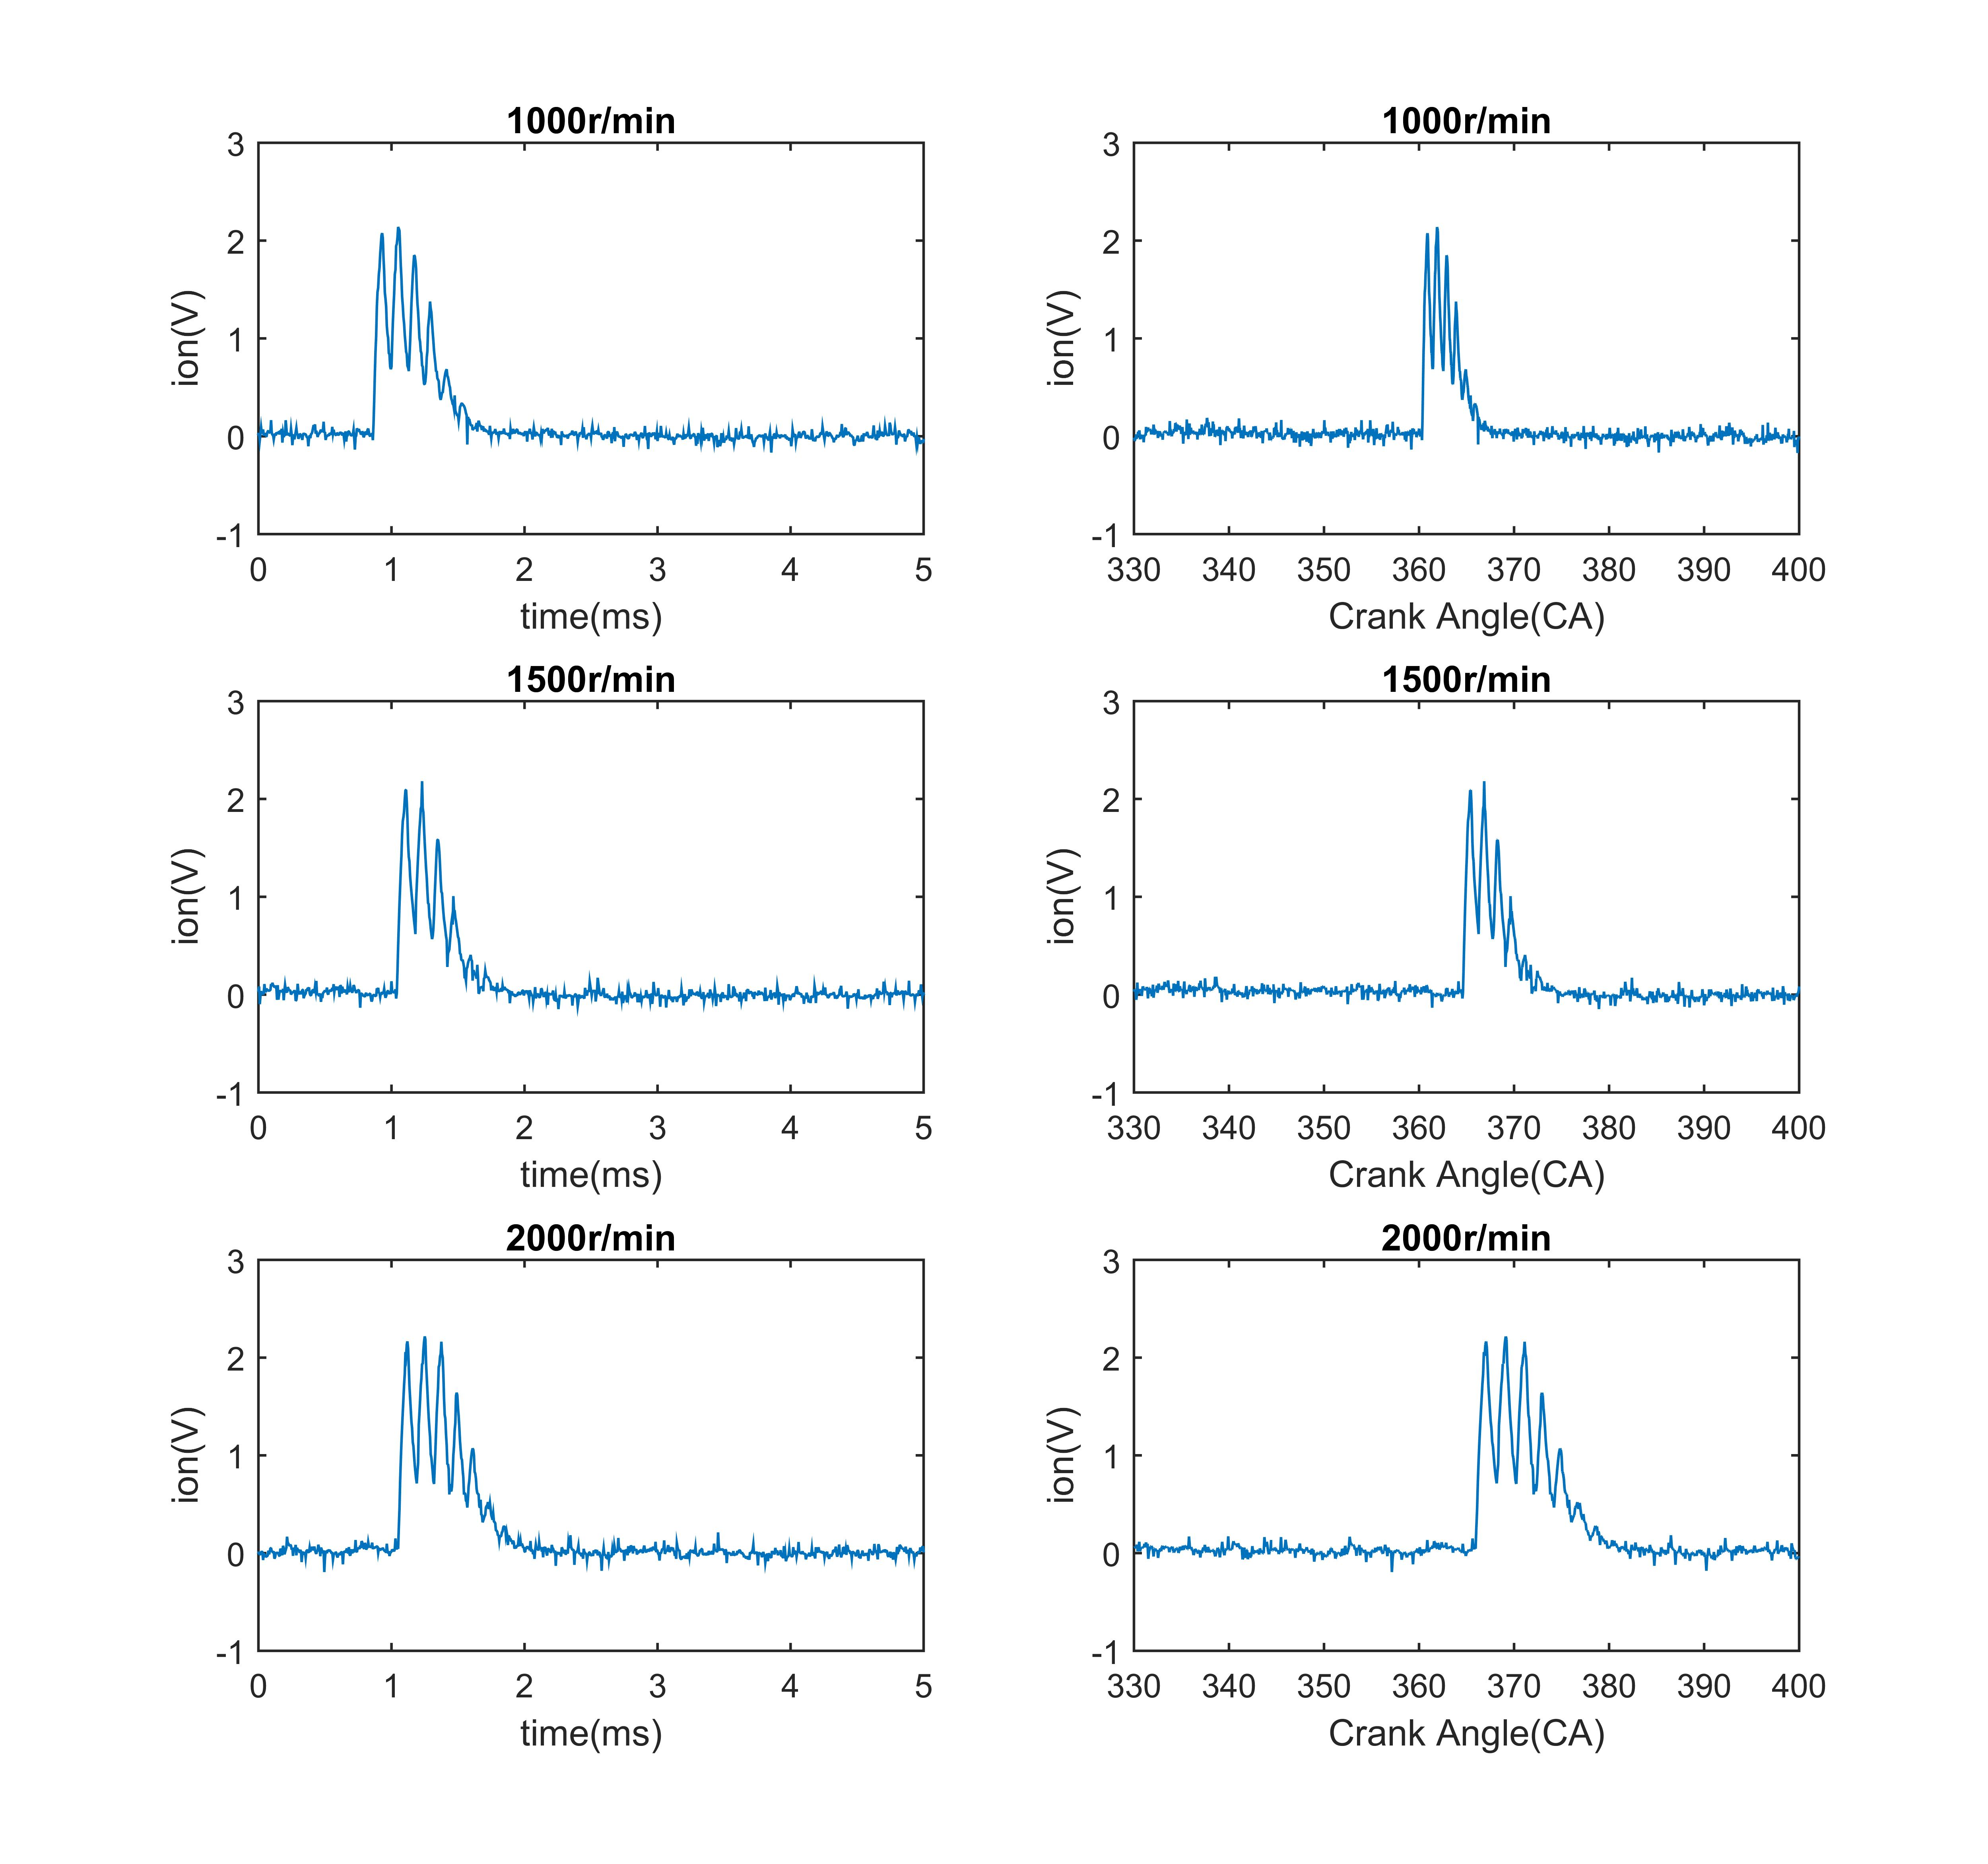
\includegraphics[width=0.9\textwidth]{thesis_figure/ion_chapter/pure_ign_comparison}
	\caption{三种转速下的纯点火干扰的时间窗口对比和曲轴转角窗口对比}
	\label{fig:pure_ign_comparison}
\end{figure}
\par为了验证该信号的偶然性,我们选取了$1250r/min,1500r/min,2000r/min$三种转速下50\%负荷情况下的同一次实验中同时进行断油和断火操作,得到三个纯点火干扰信号。
从图\ref{fig:pure_ign_comparison}中可以看到纯点火干扰在时间窗口上具有很相近的形状,但是仍然有细节上的差异,如果用正常信号直接减去该纯点火干扰信号并不能非常完美的呈现出离子电流信号。有必要通过
其他的信号分析手段来将该点火干扰信号剔除。
\section{四种小波基函数对点火干扰进行小波分析}
小波分析的方法可以很好的将高频信号和低频信号进行分离,我们采用db,sym,coif,dmey四种离散小波基函数对纯电火干扰信号进行分析,将纯点火干扰信号中的震荡信号去除。
\begin{figure}[!htb]
	\begin{tabular}{lll}
		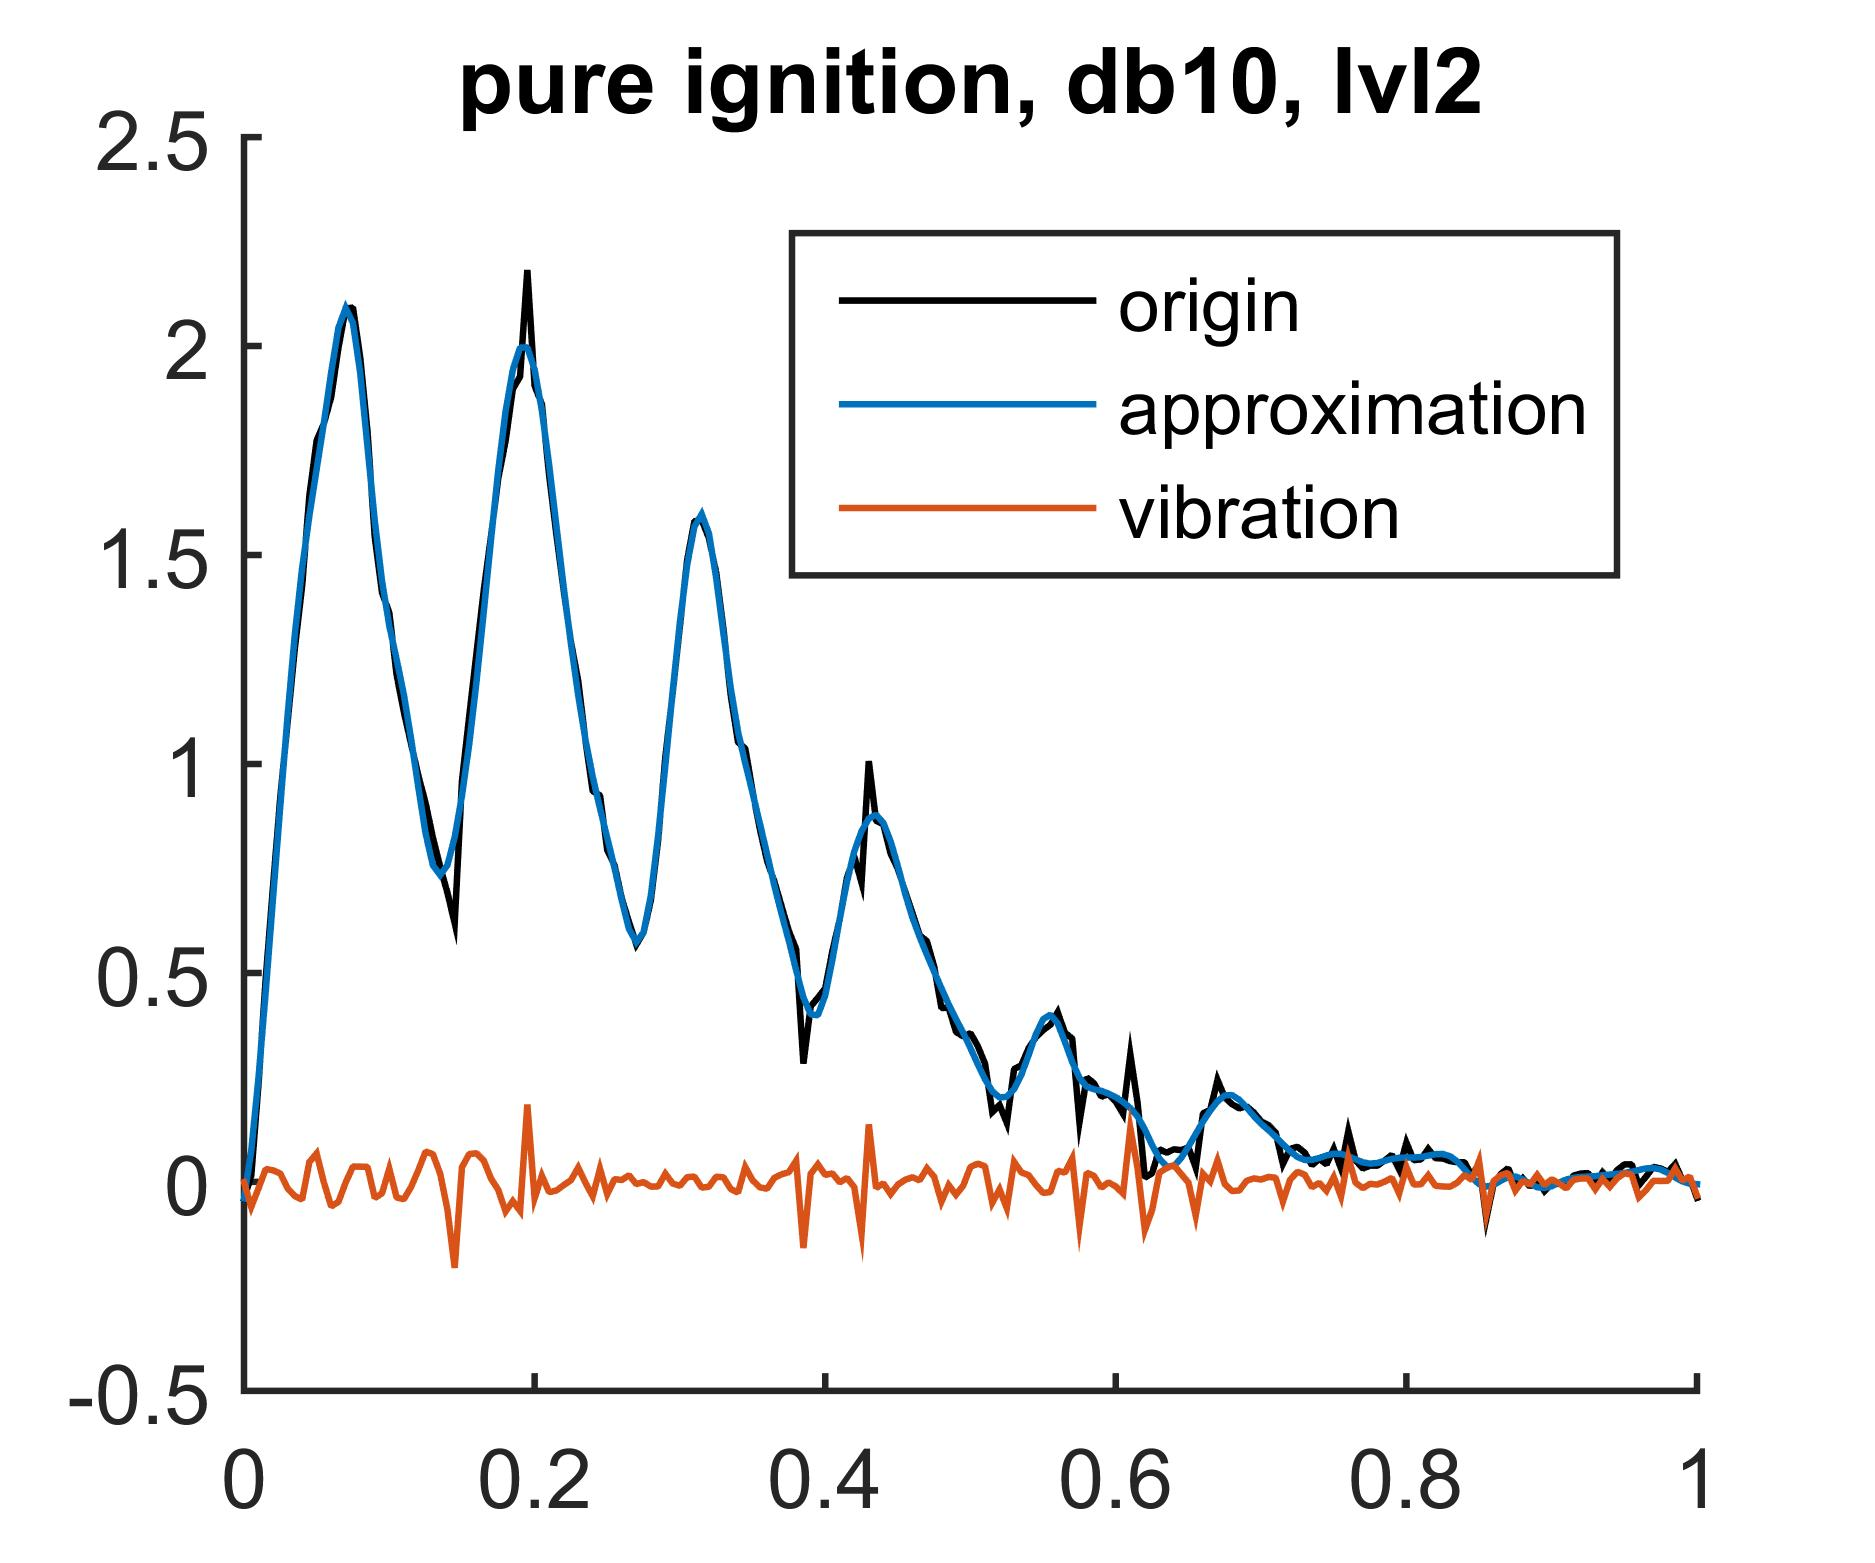
\includegraphics[width=0.3\textwidth]{thesis_figure/ion_chapter/db10_lvl2}&
		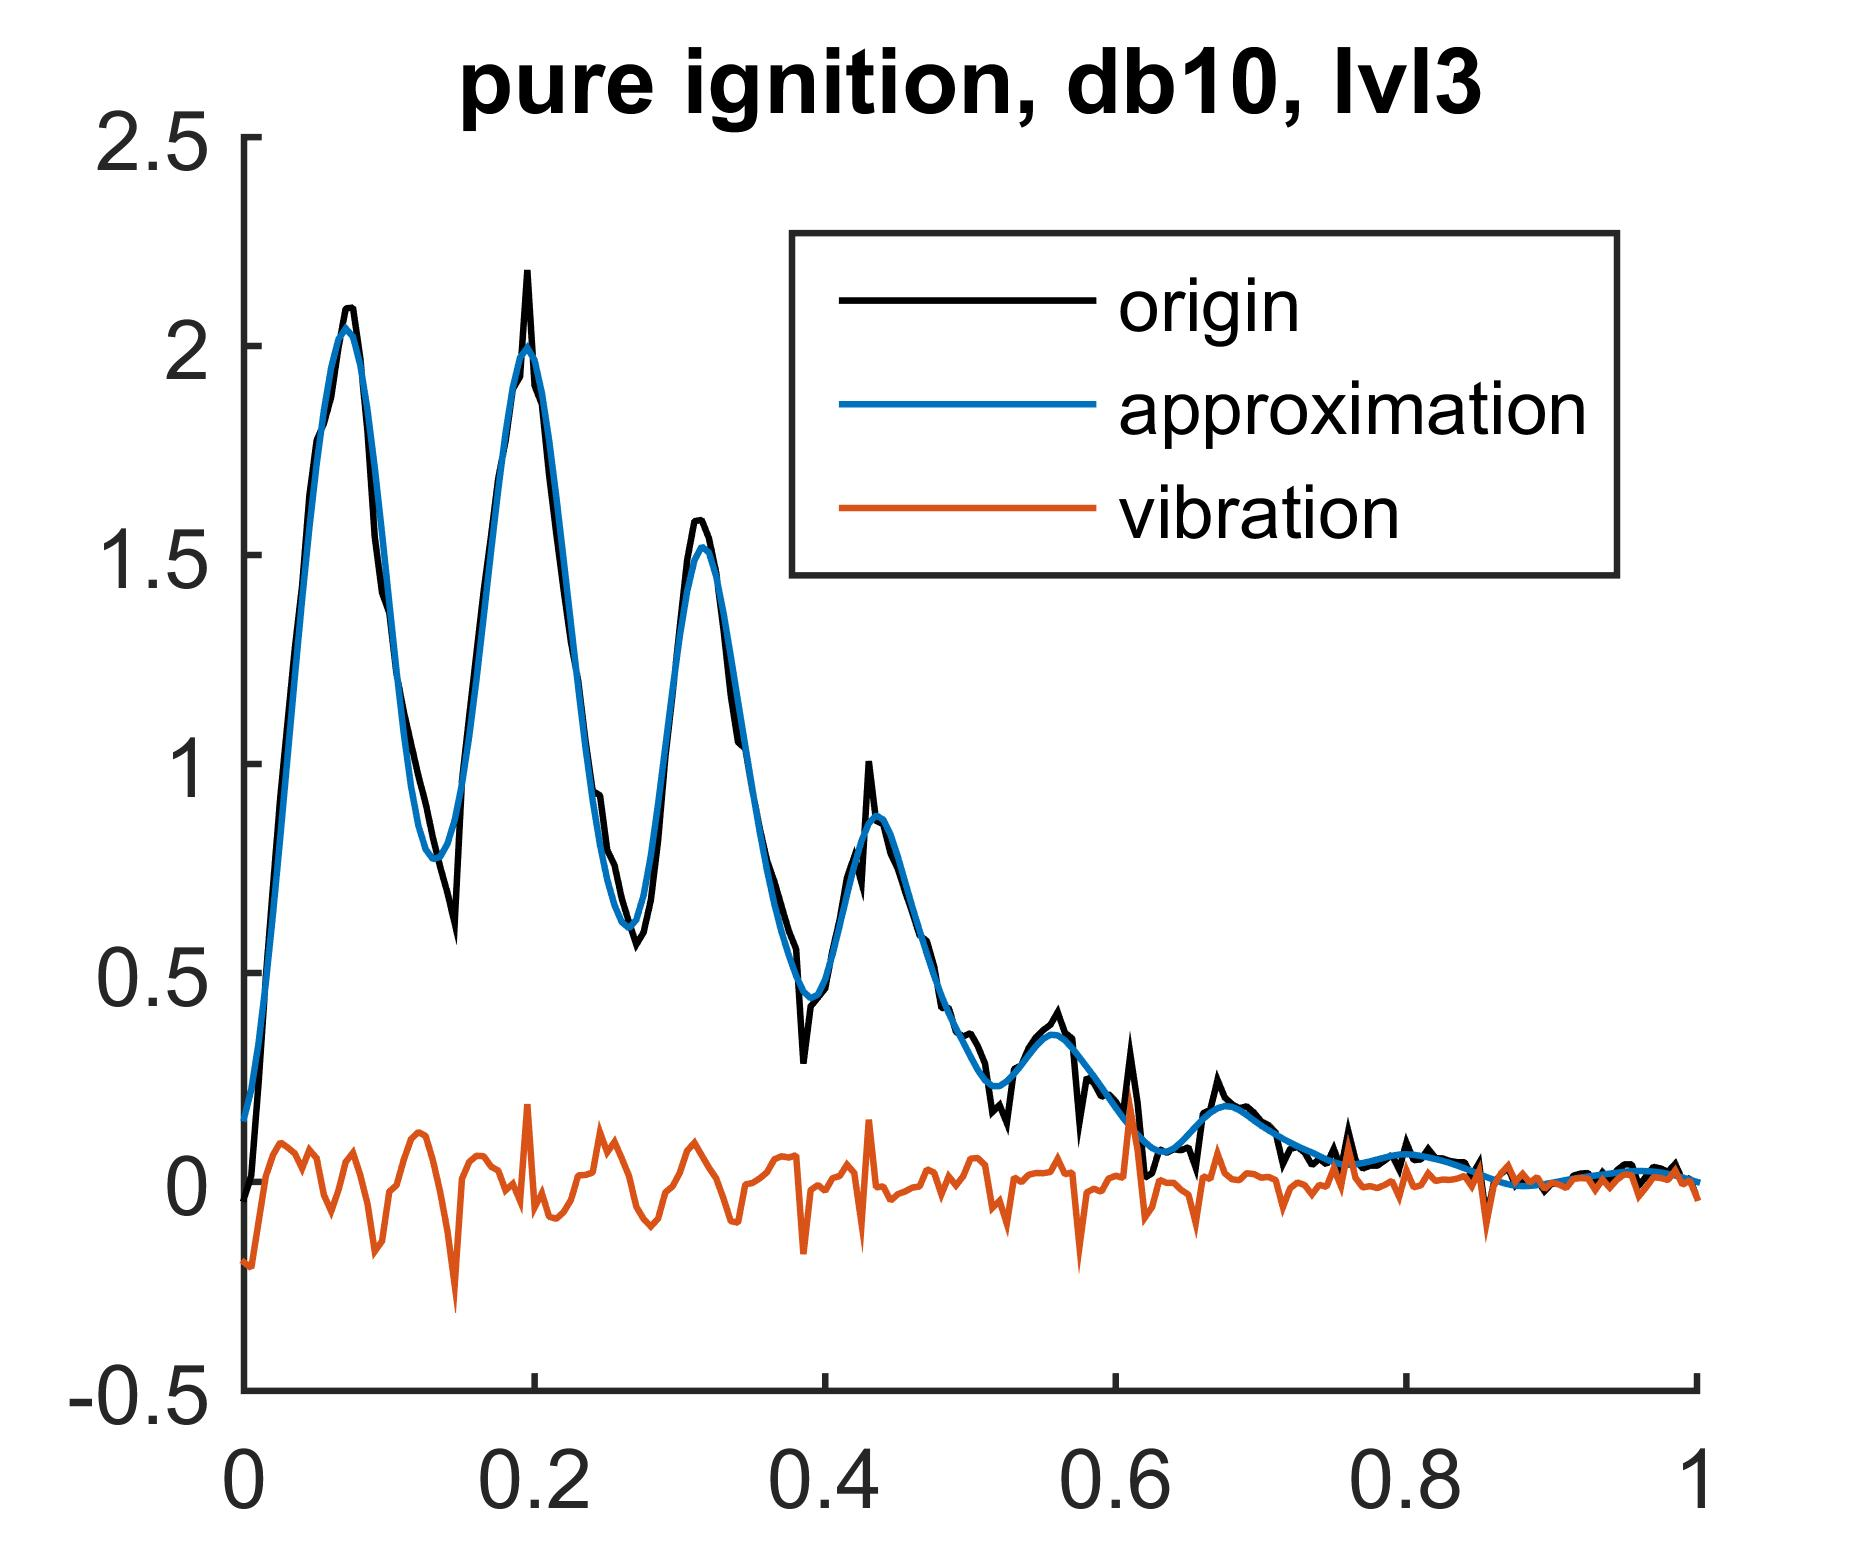
\includegraphics[width=0.3\textwidth]{thesis_figure/ion_chapter/db10_lvl3}&
		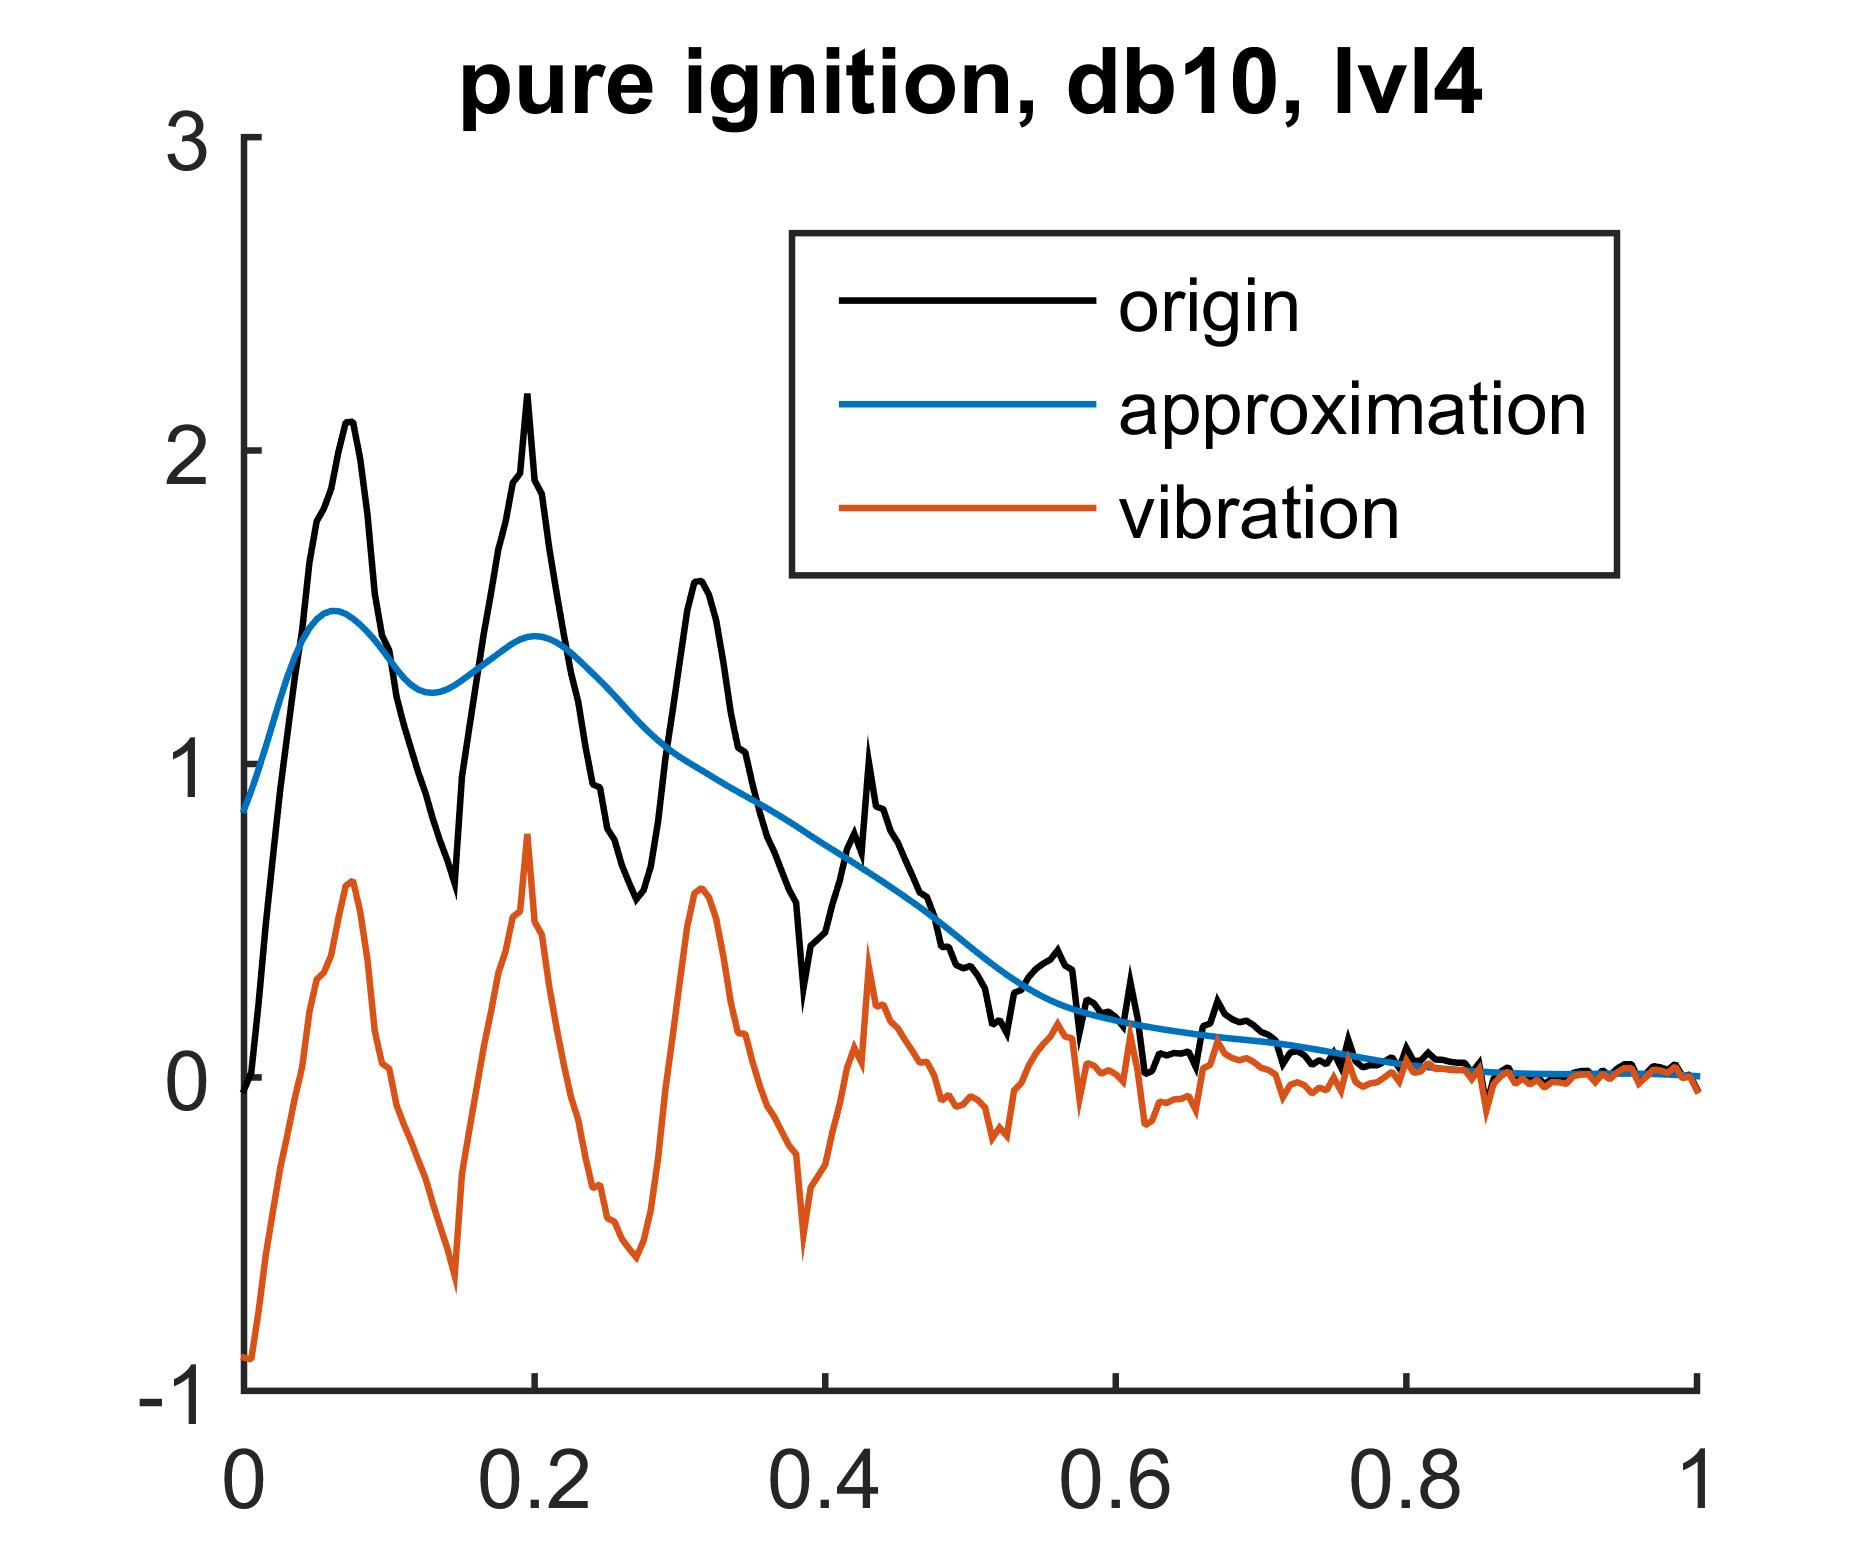
\includegraphics[width=0.3\textwidth]{thesis_figure/ion_chapter/db10_lvl4}\\
		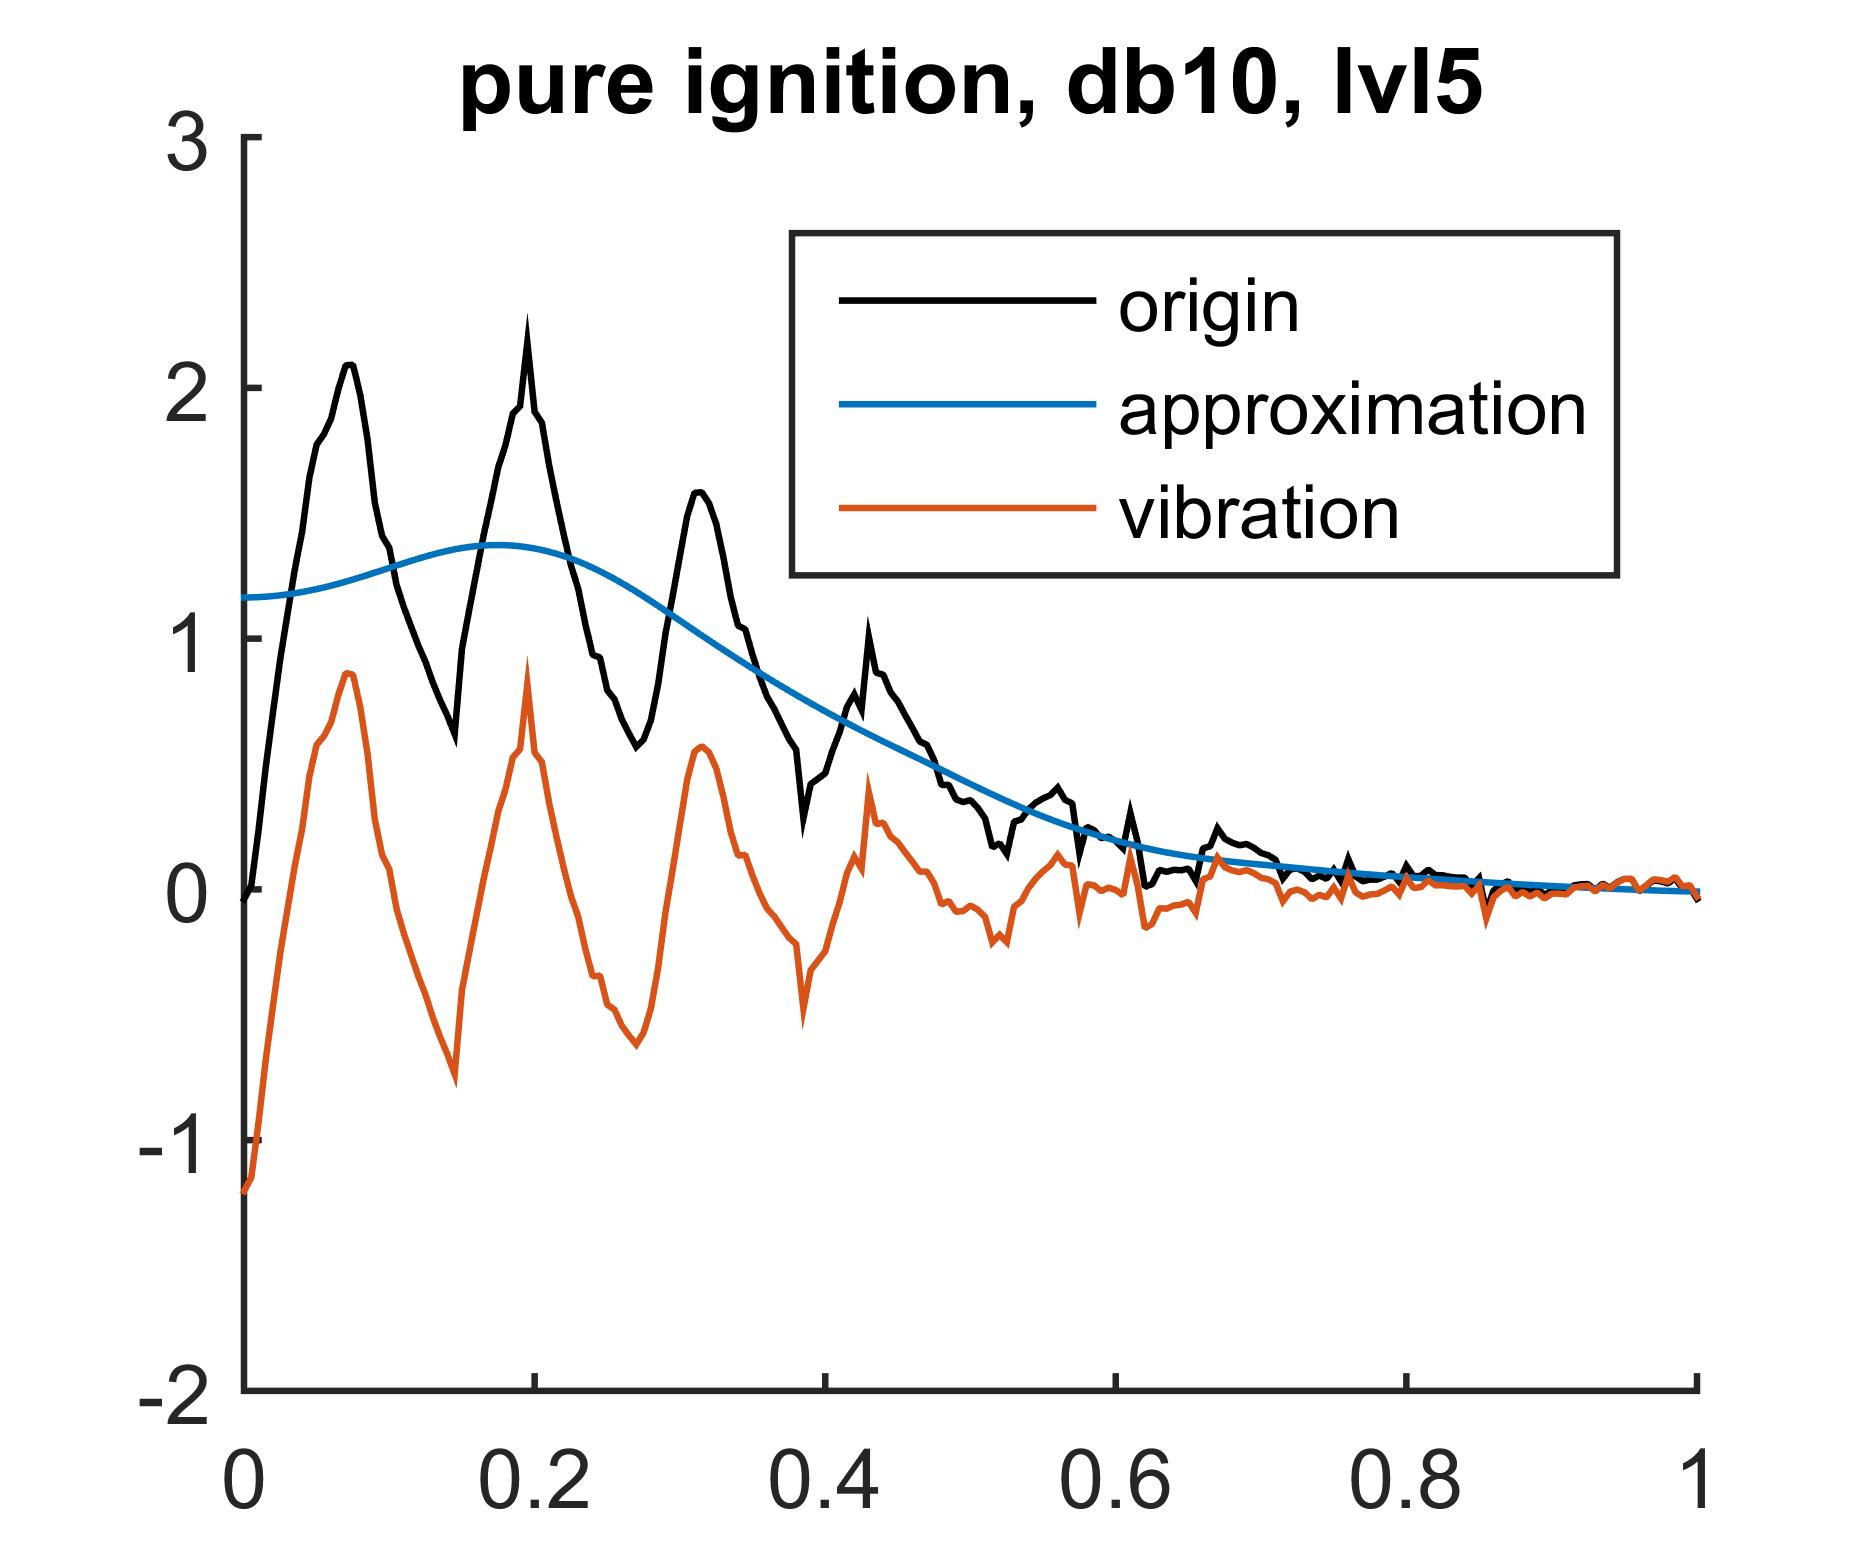
\includegraphics[width=0.3\textwidth]{thesis_figure/ion_chapter/db10_lvl5}&
		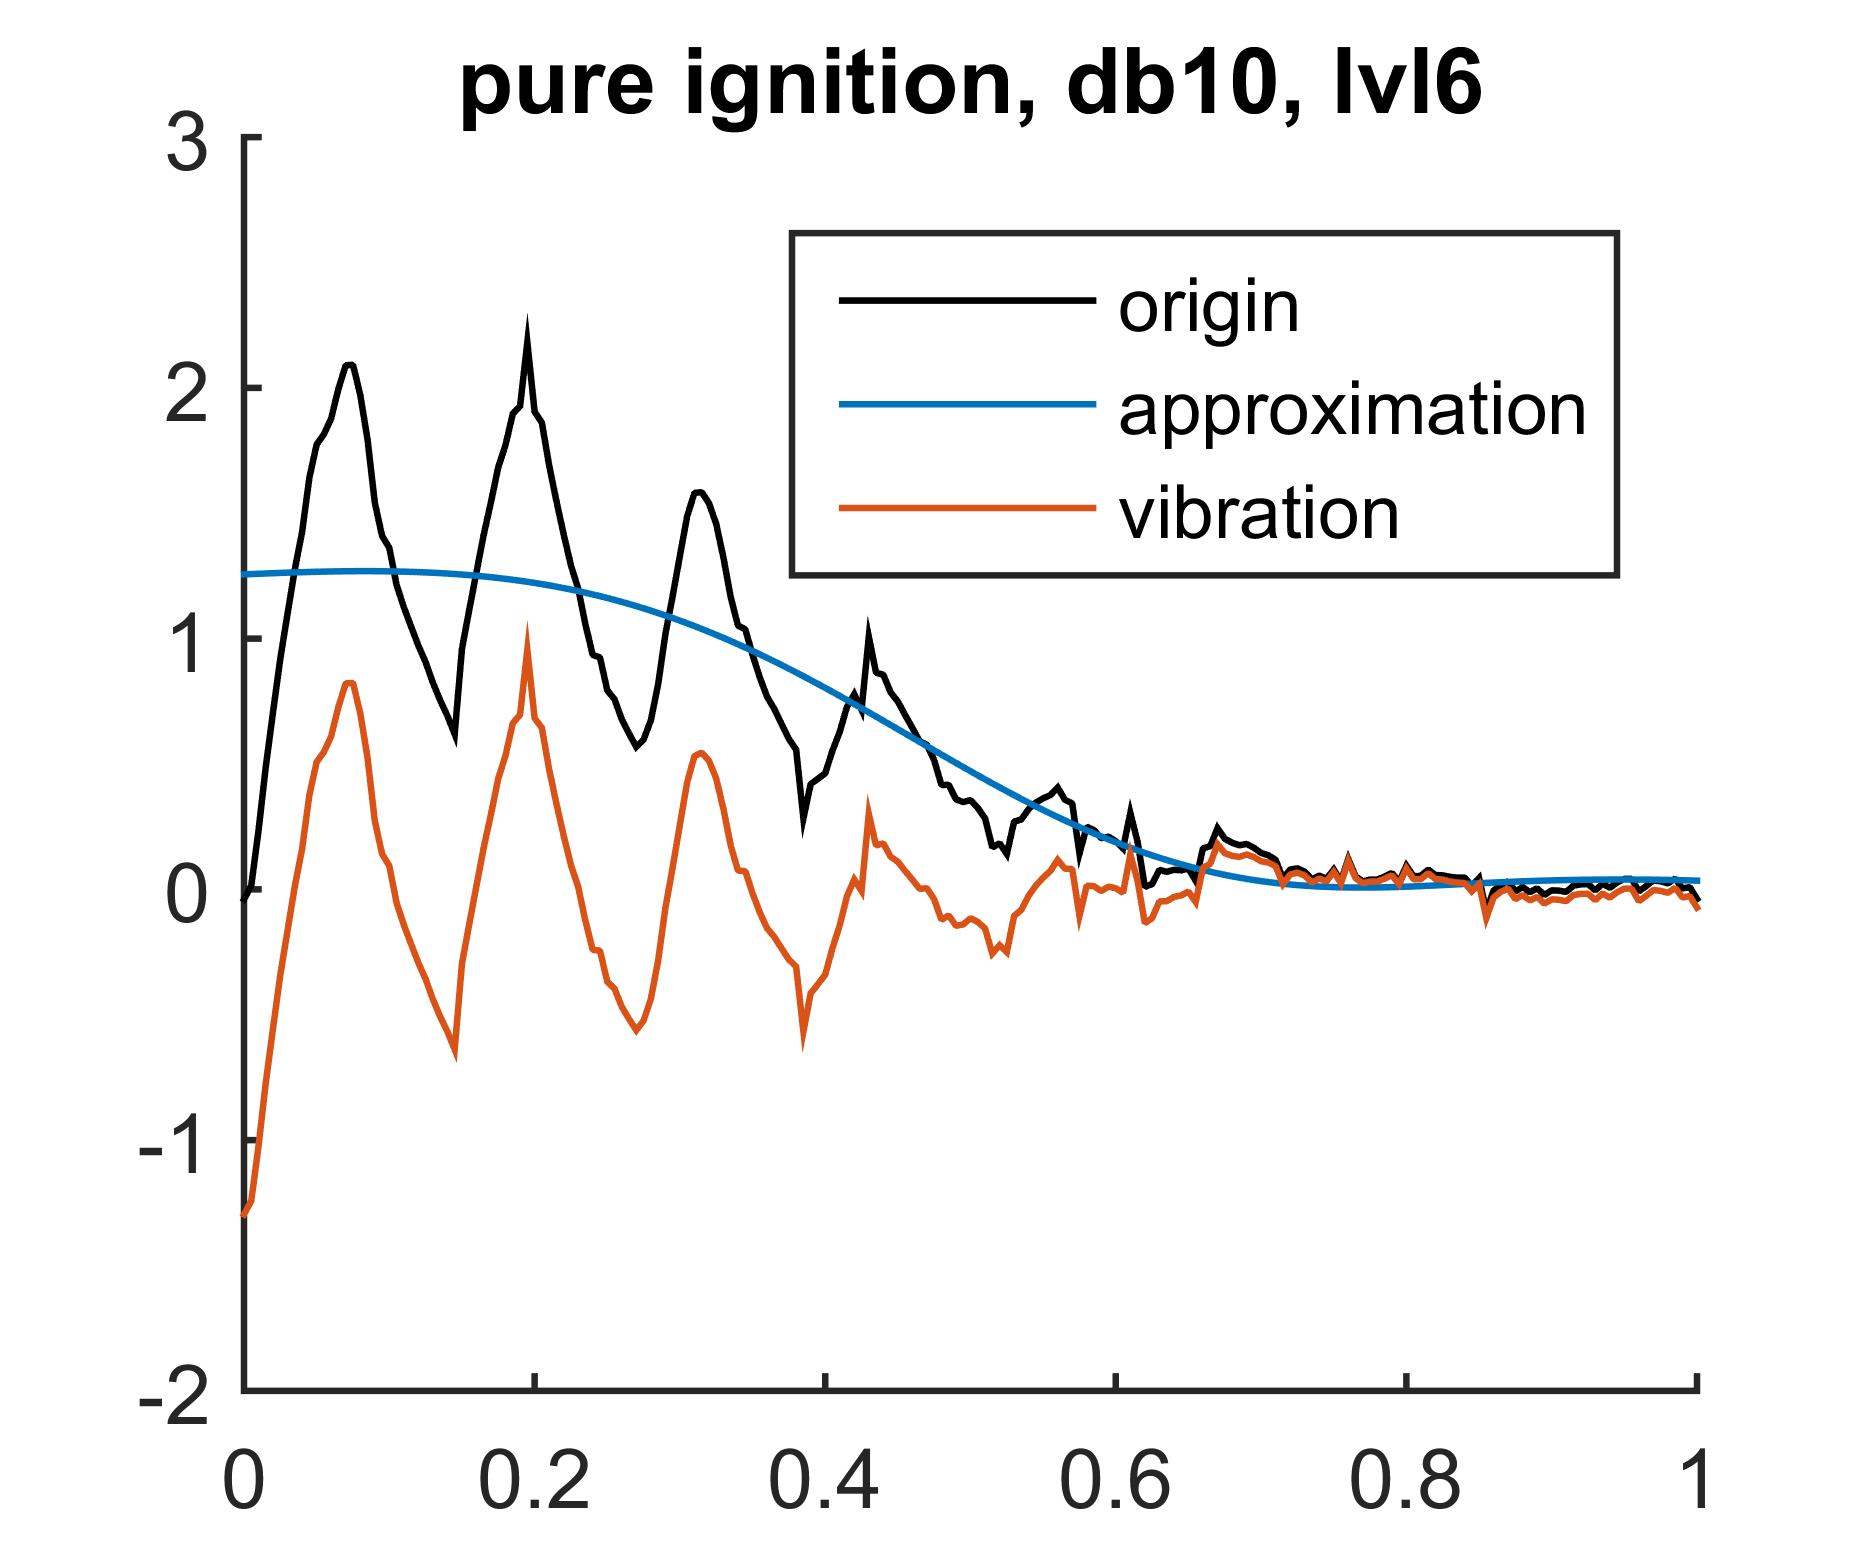
\includegraphics[width=0.3\textwidth]{thesis_figure/ion_chapter/db10_lvl6}&
		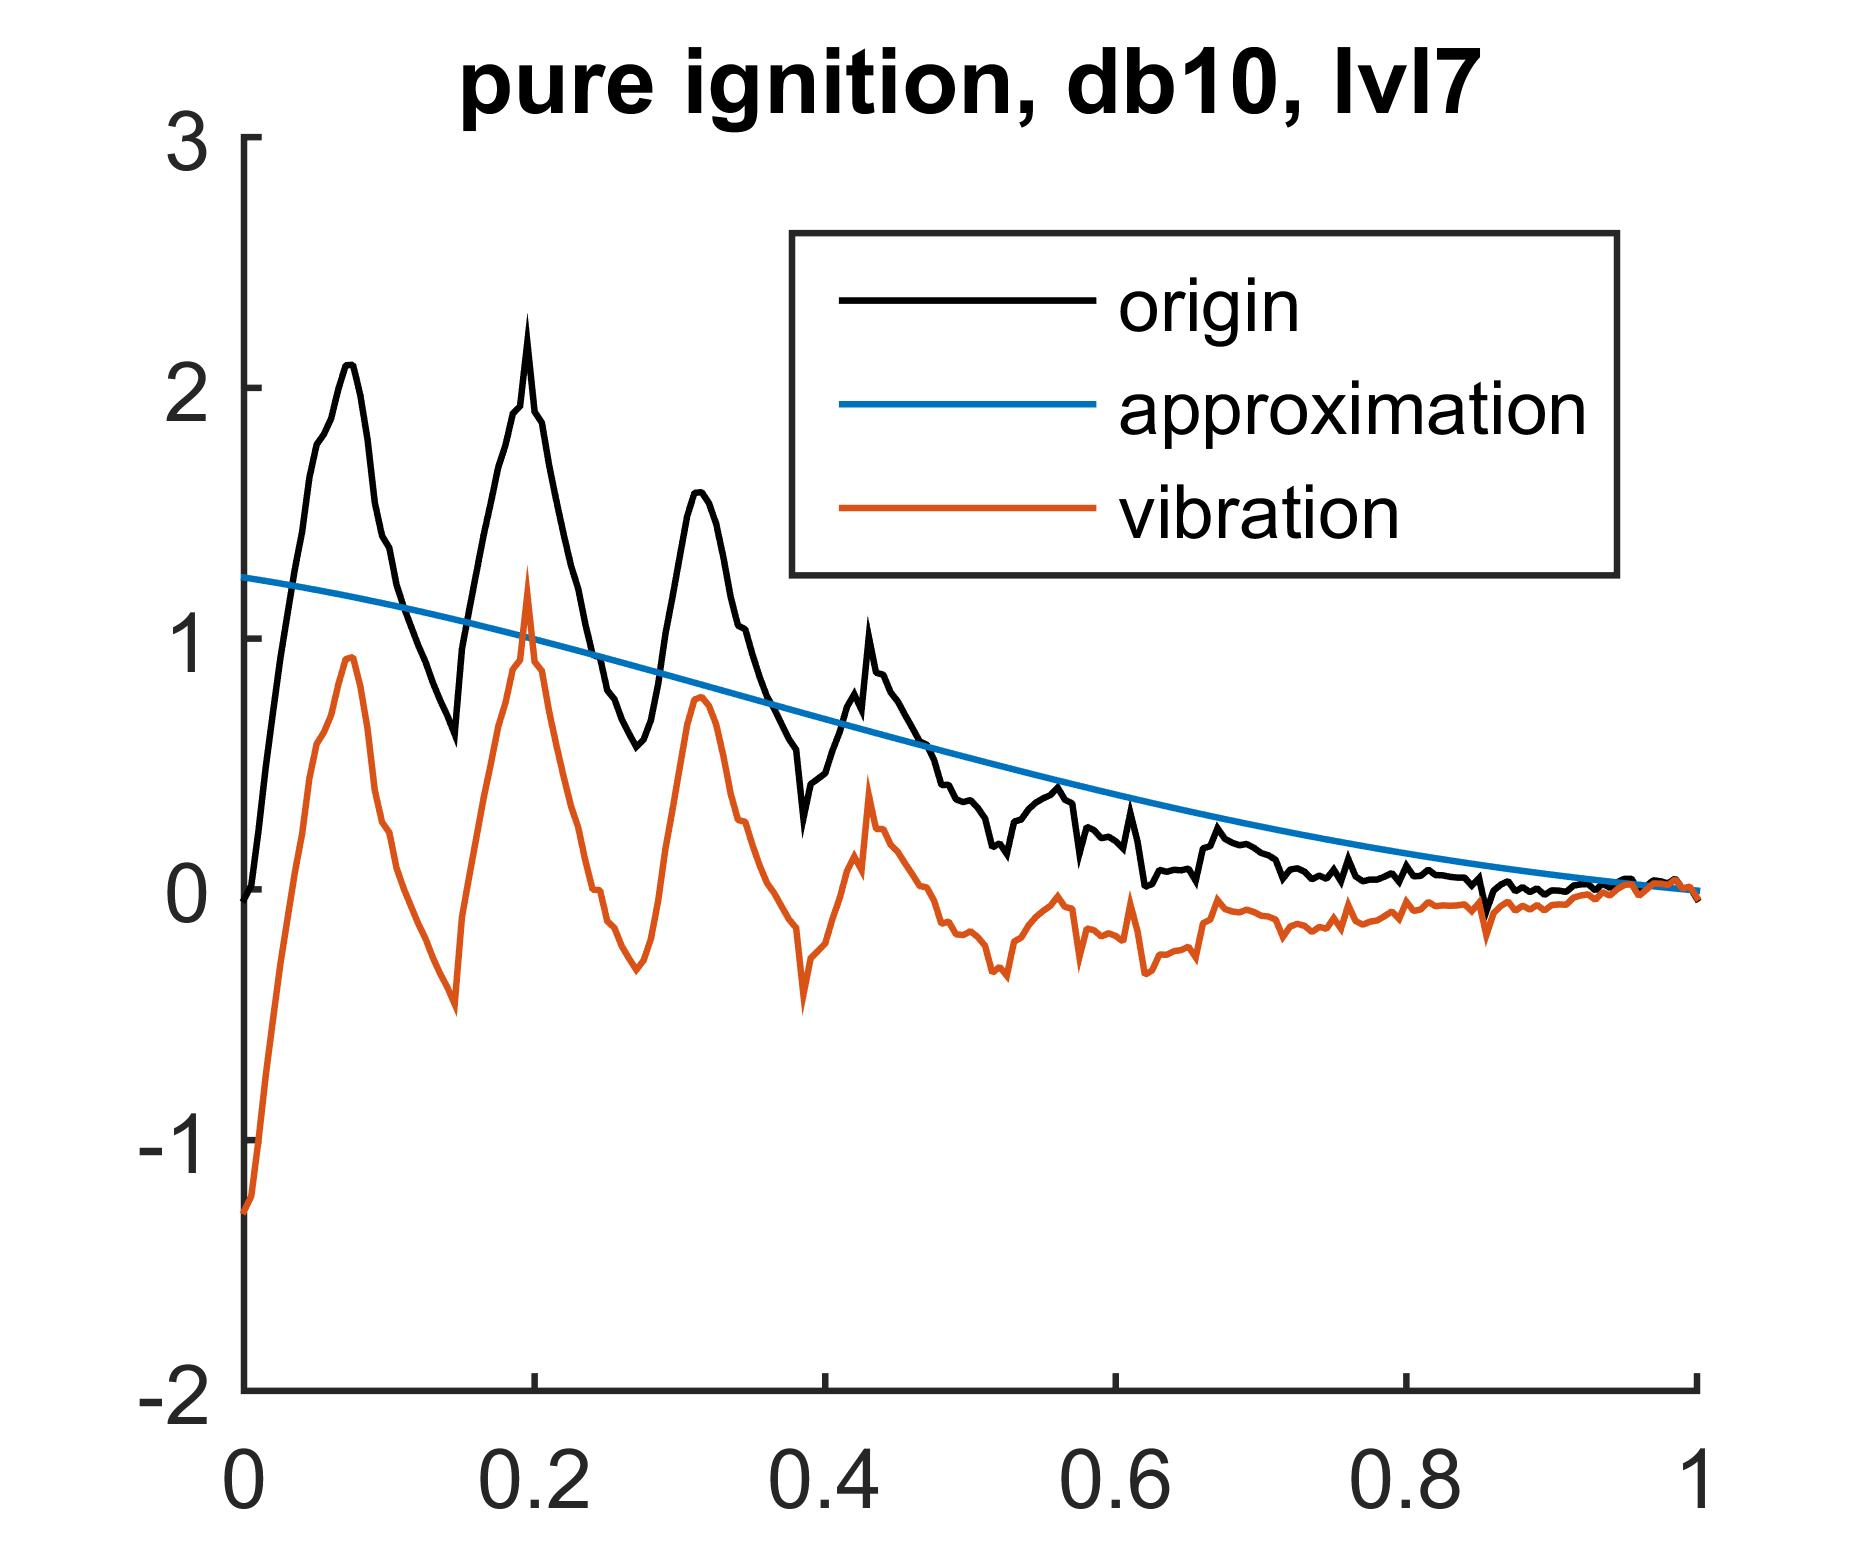
\includegraphics[width=0.3\textwidth]{thesis_figure/ion_chapter/db10_lvl7}
	\end{tabular}
	\caption{\label{fig:db10}db10小波对纯点火干扰信号进行10层分解}
\end{figure}
\par先用db10小波对纯点火干扰信号进行10层分解,观察第二层到第七层的分解情况,如图\ref{fig:db10}所示,可以看到第二层和第三层并没有将震荡信号分解开来,而第六层和第七层分解出来的平滑信号过
于硬直,且分解的震荡信号不具有很好的衰减特性。而第四层分解相对于第五层分解来说,效果没有那么理想。所以本文以下的小波分析都是基于第五层分解来进行的。由于dmey没有阶数问题,而coif小波
的最高阶数为5。所以只讨论db小波和sym小波的阶数问题。
\subsection{db小波族的阶数选择和分析}
取阶数分别为5、10、15、20、25和30的db小波对纯干扰信号进行分析。
\begin{figure}[!htb]
	\centering
	\begin{tabular}{ccc}
		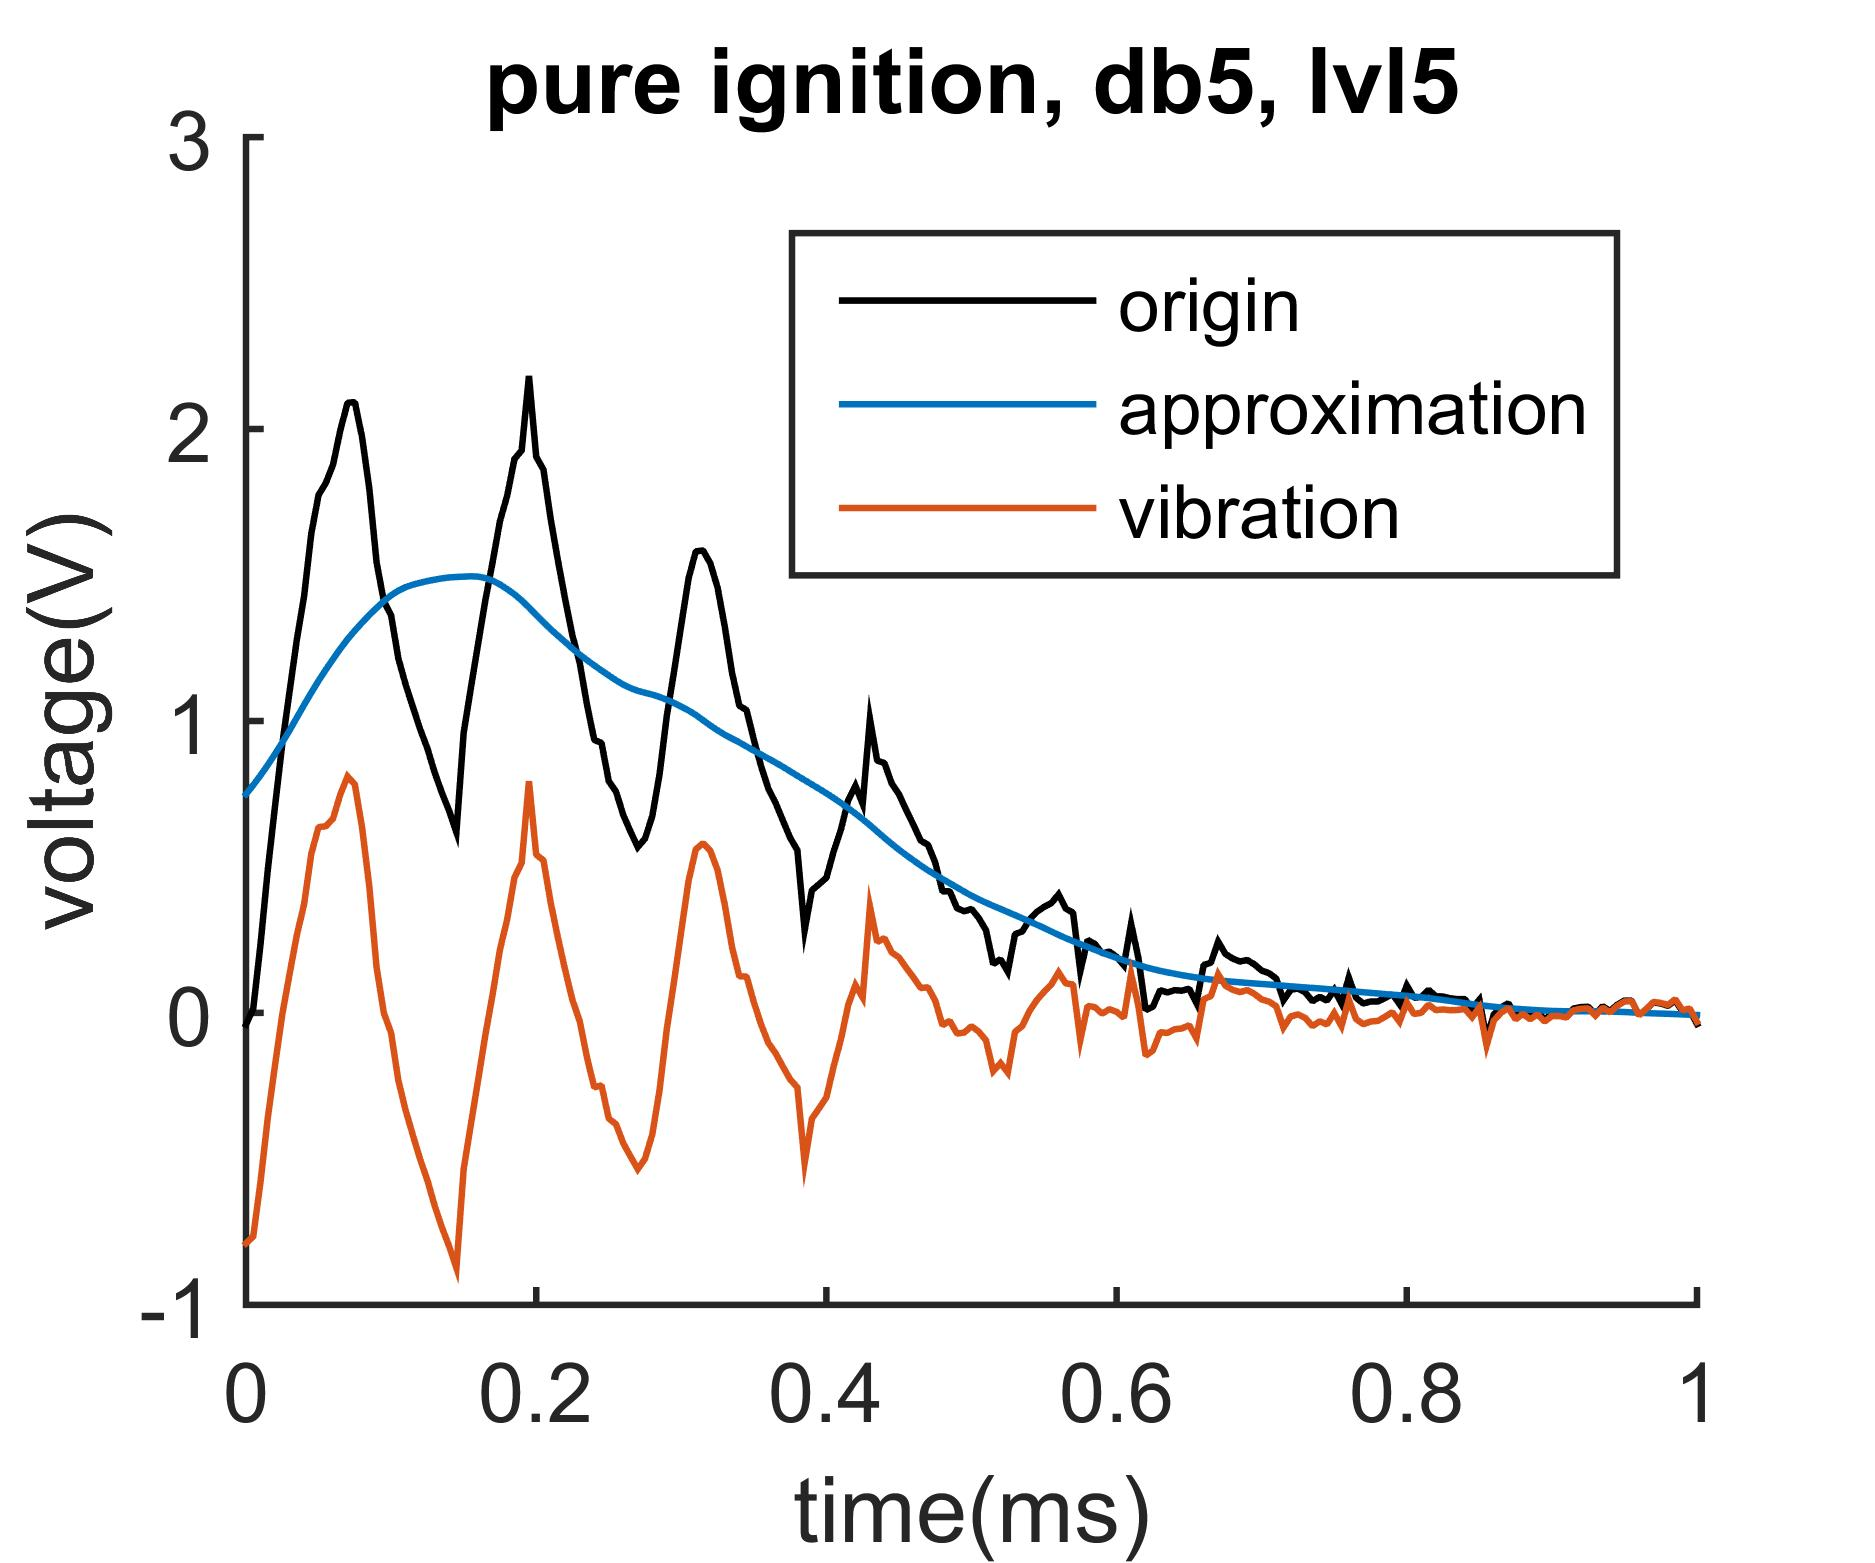
\includegraphics[width=0.3\textwidth]{thesis_figure/ion_chapter/db5_lvl5}&
		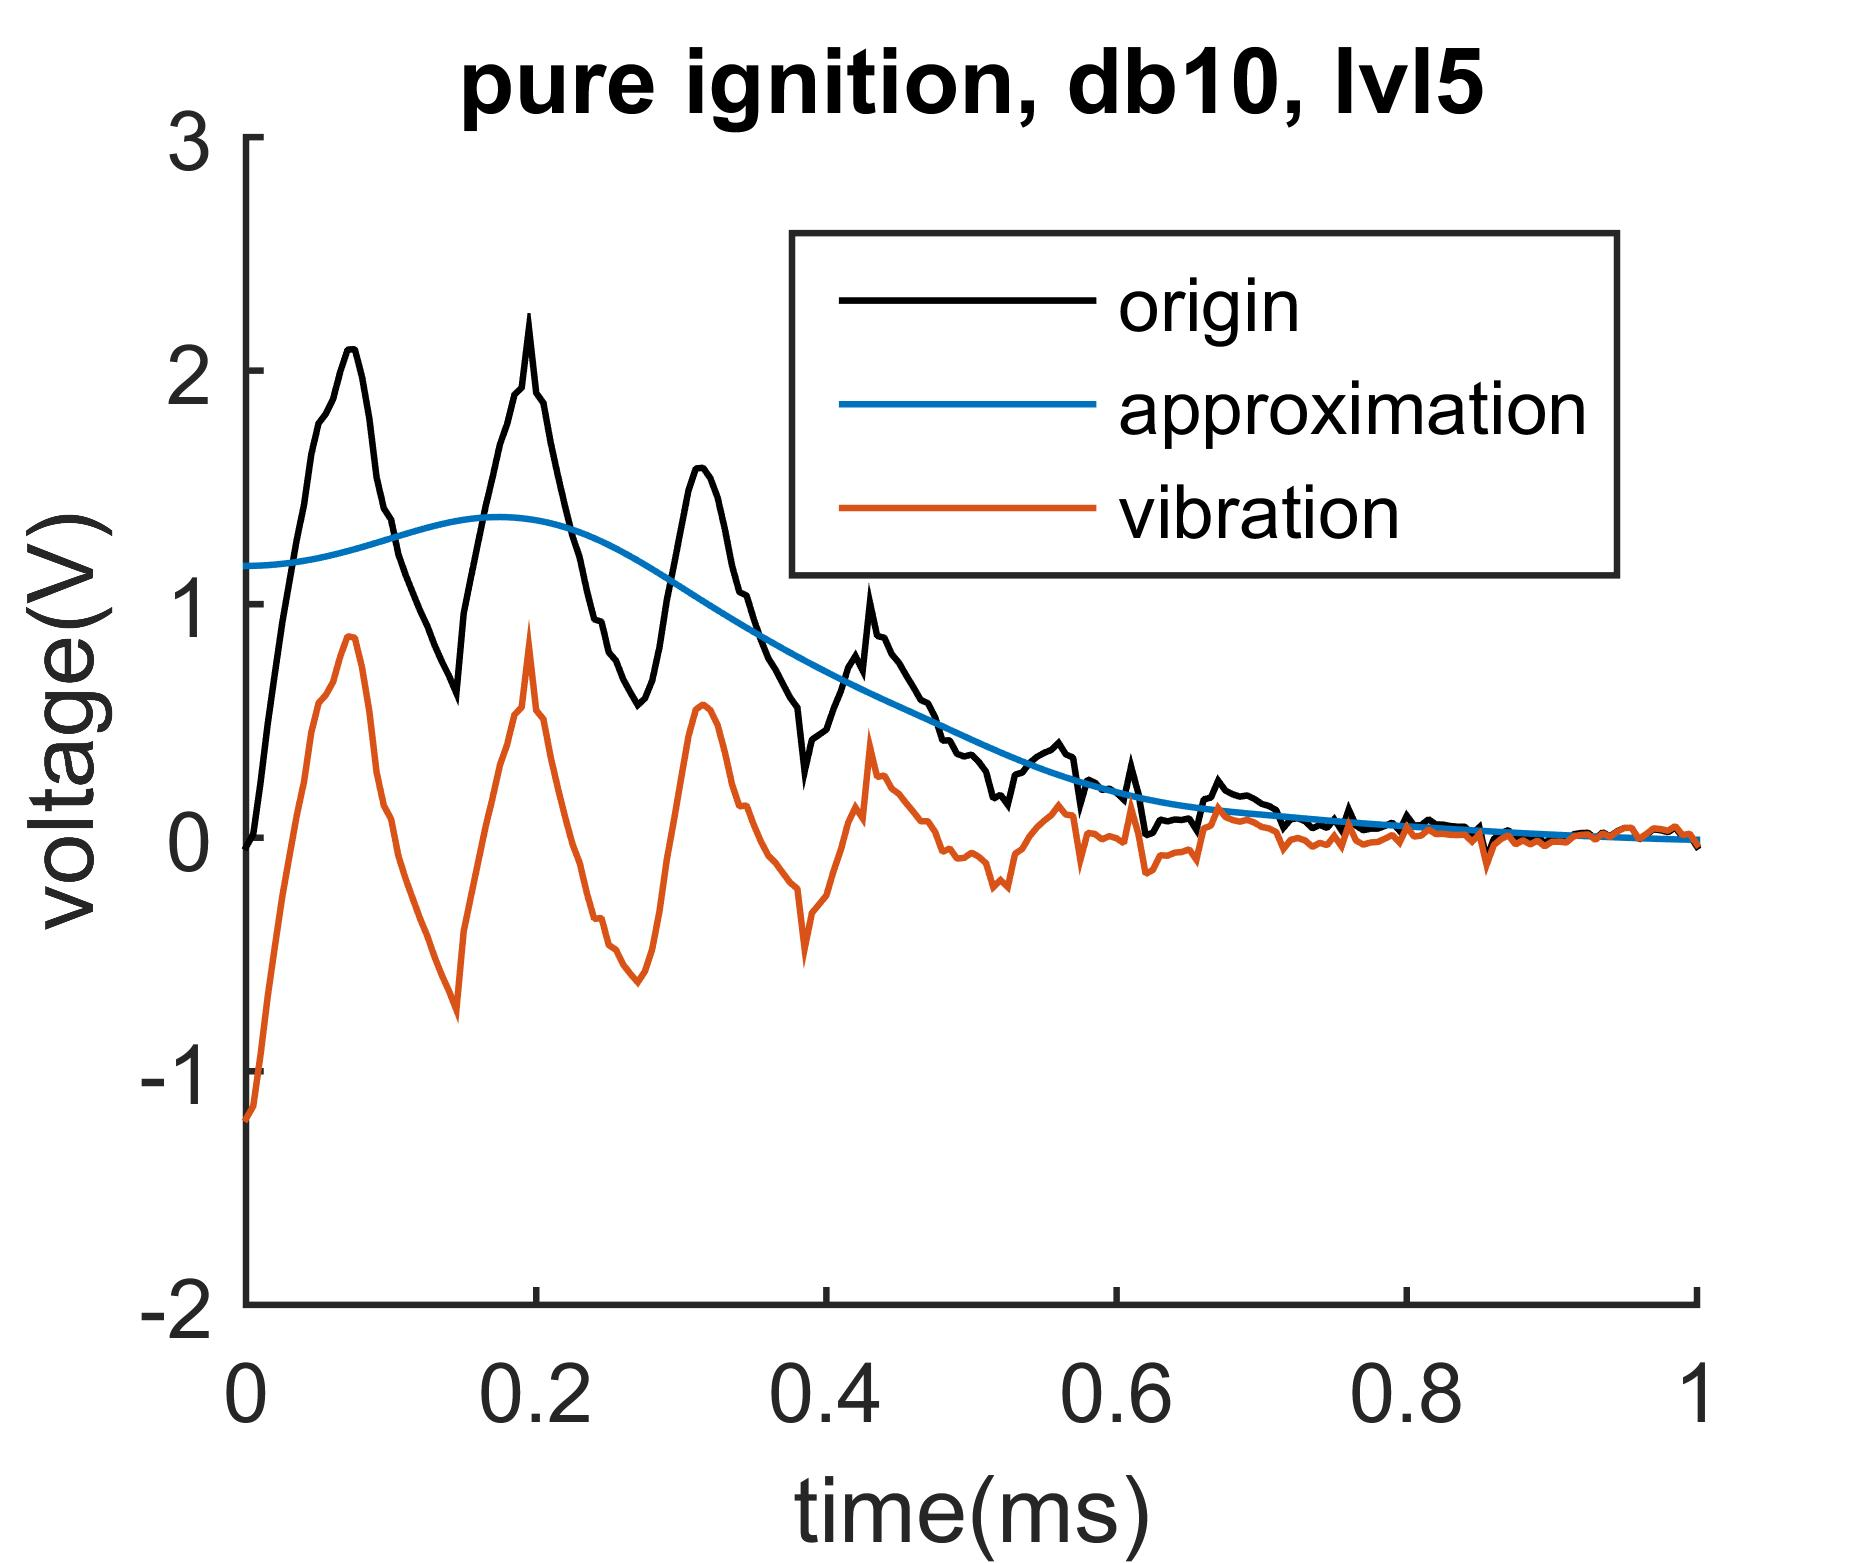
\includegraphics[width=0.3\textwidth]{thesis_figure/ion_chapter/db10_lvl5_1}&
		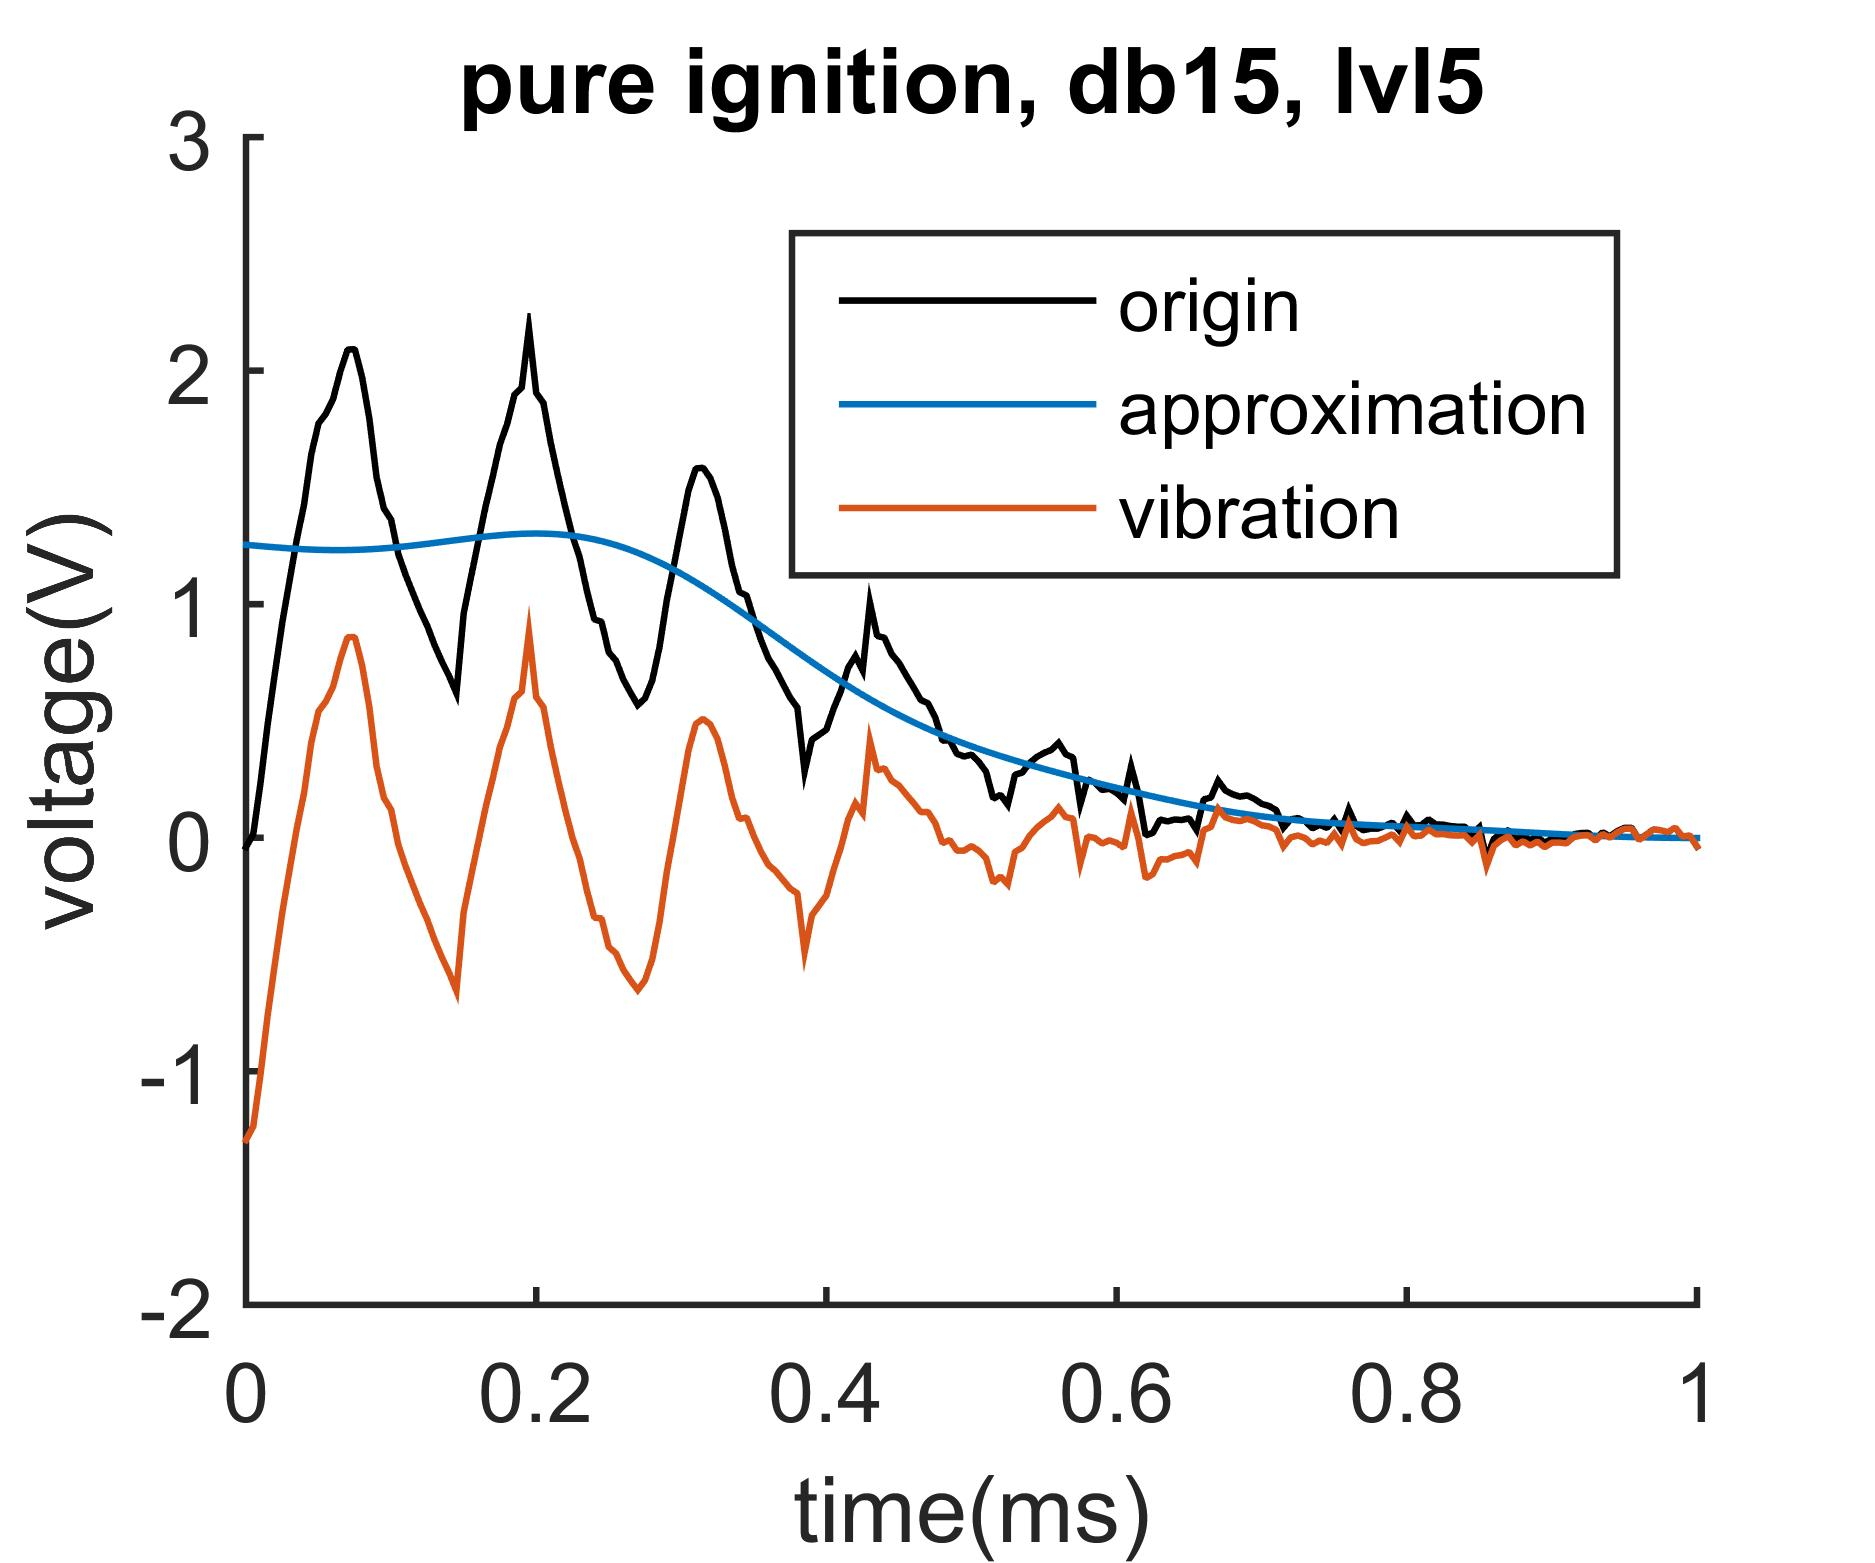
\includegraphics[width=0.3\textwidth]{thesis_figure/ion_chapter/db15_lvl5}\\
		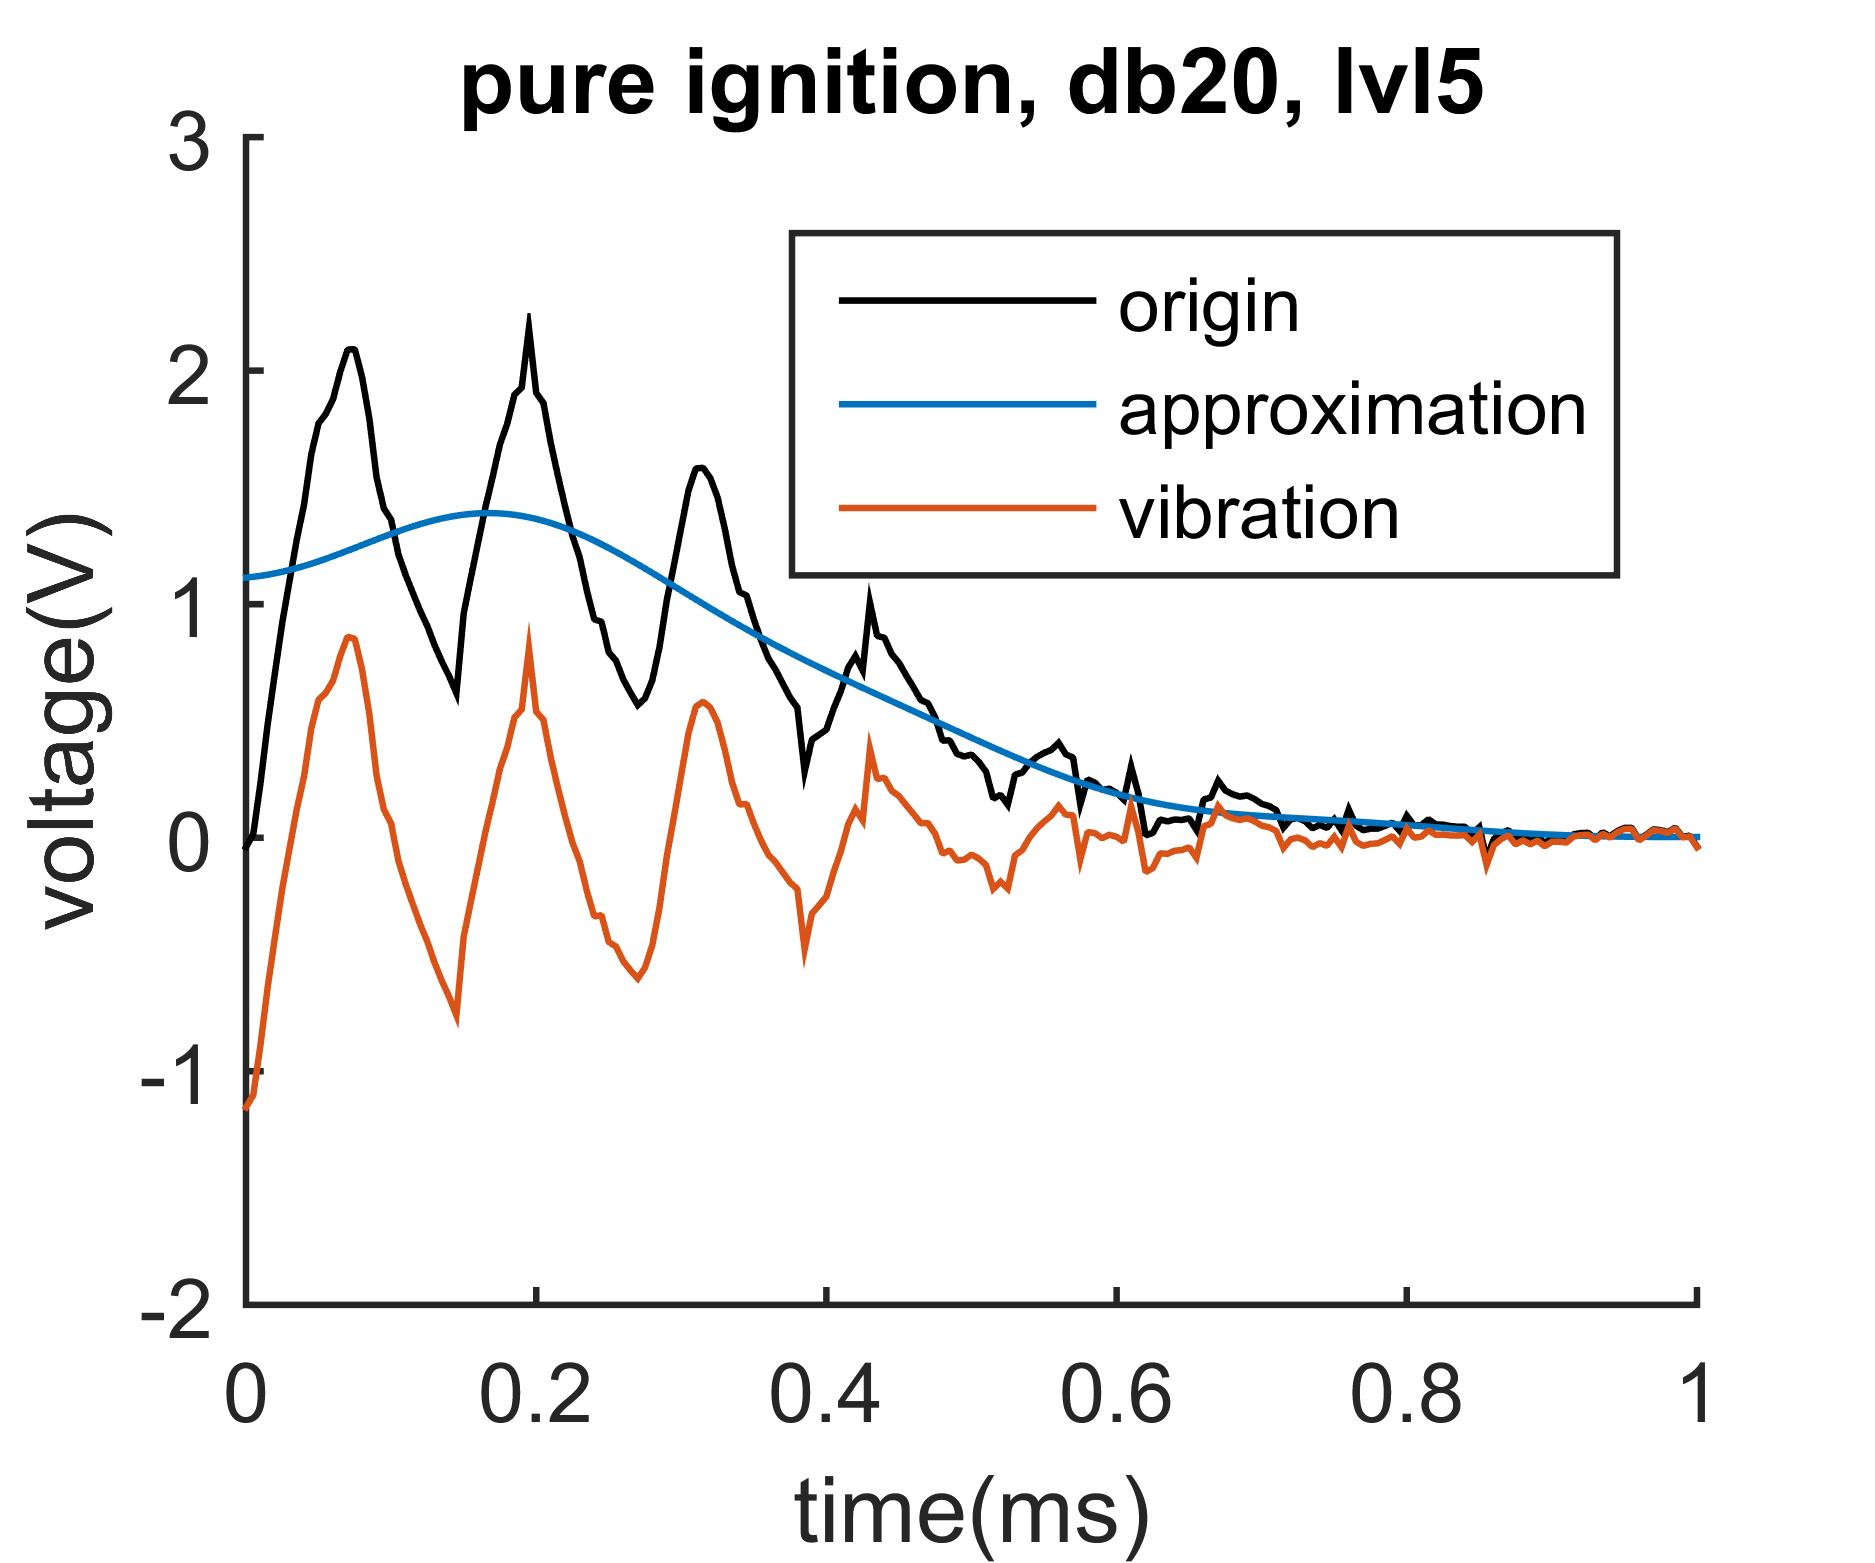
\includegraphics[width=0.3\textwidth]{thesis_figure/ion_chapter/db20_lvl5}&
		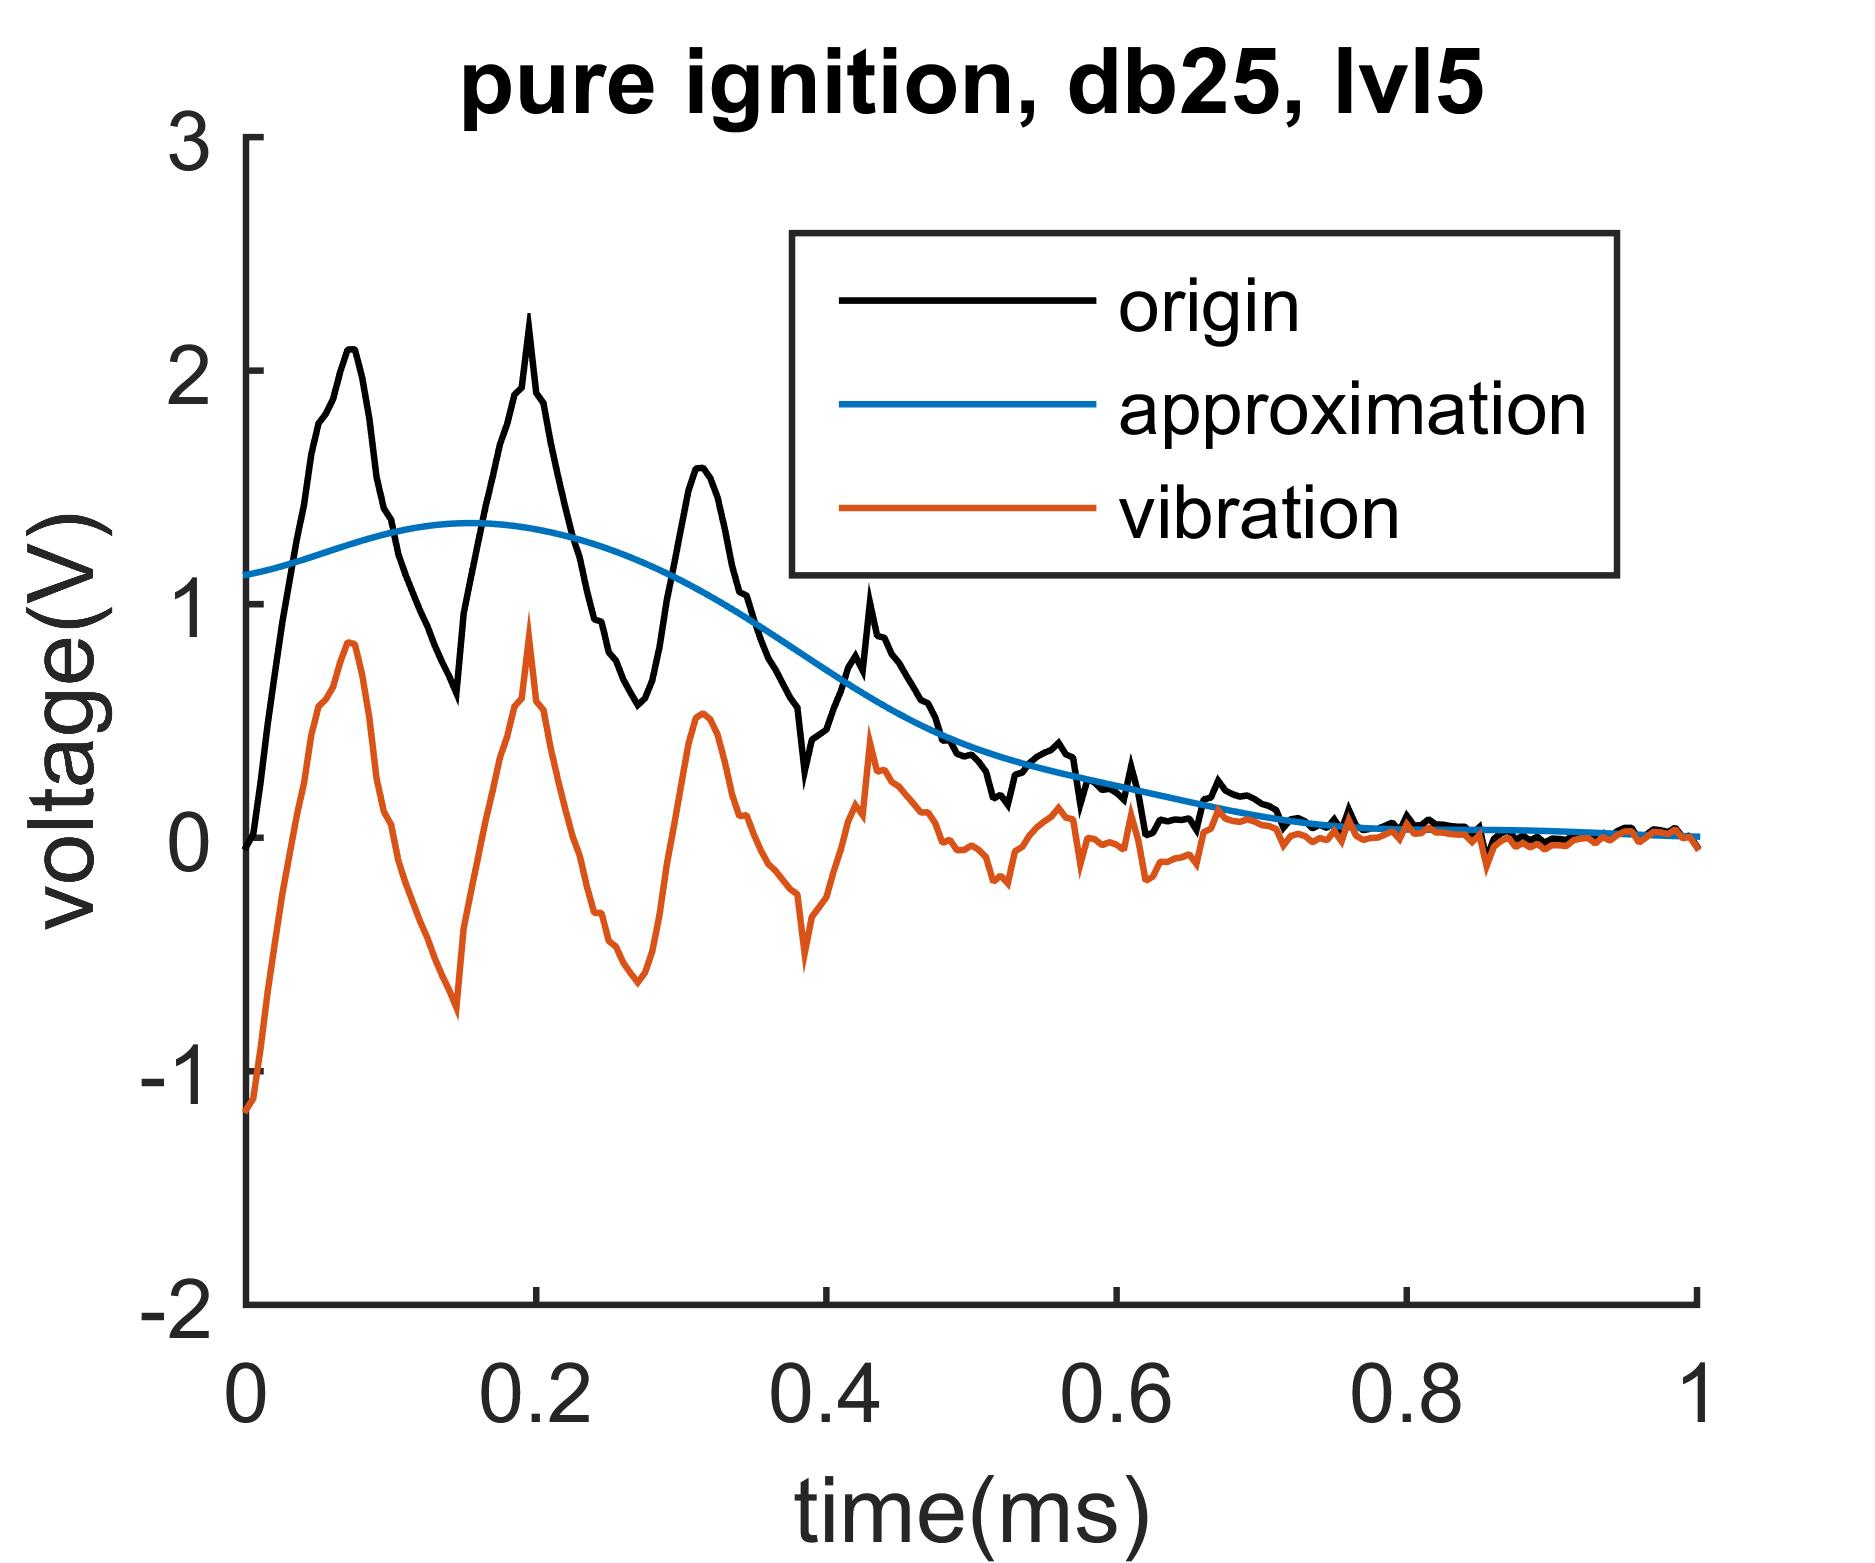
\includegraphics[width=0.3\textwidth]{thesis_figure/ion_chapter/db25_lvl5}&
		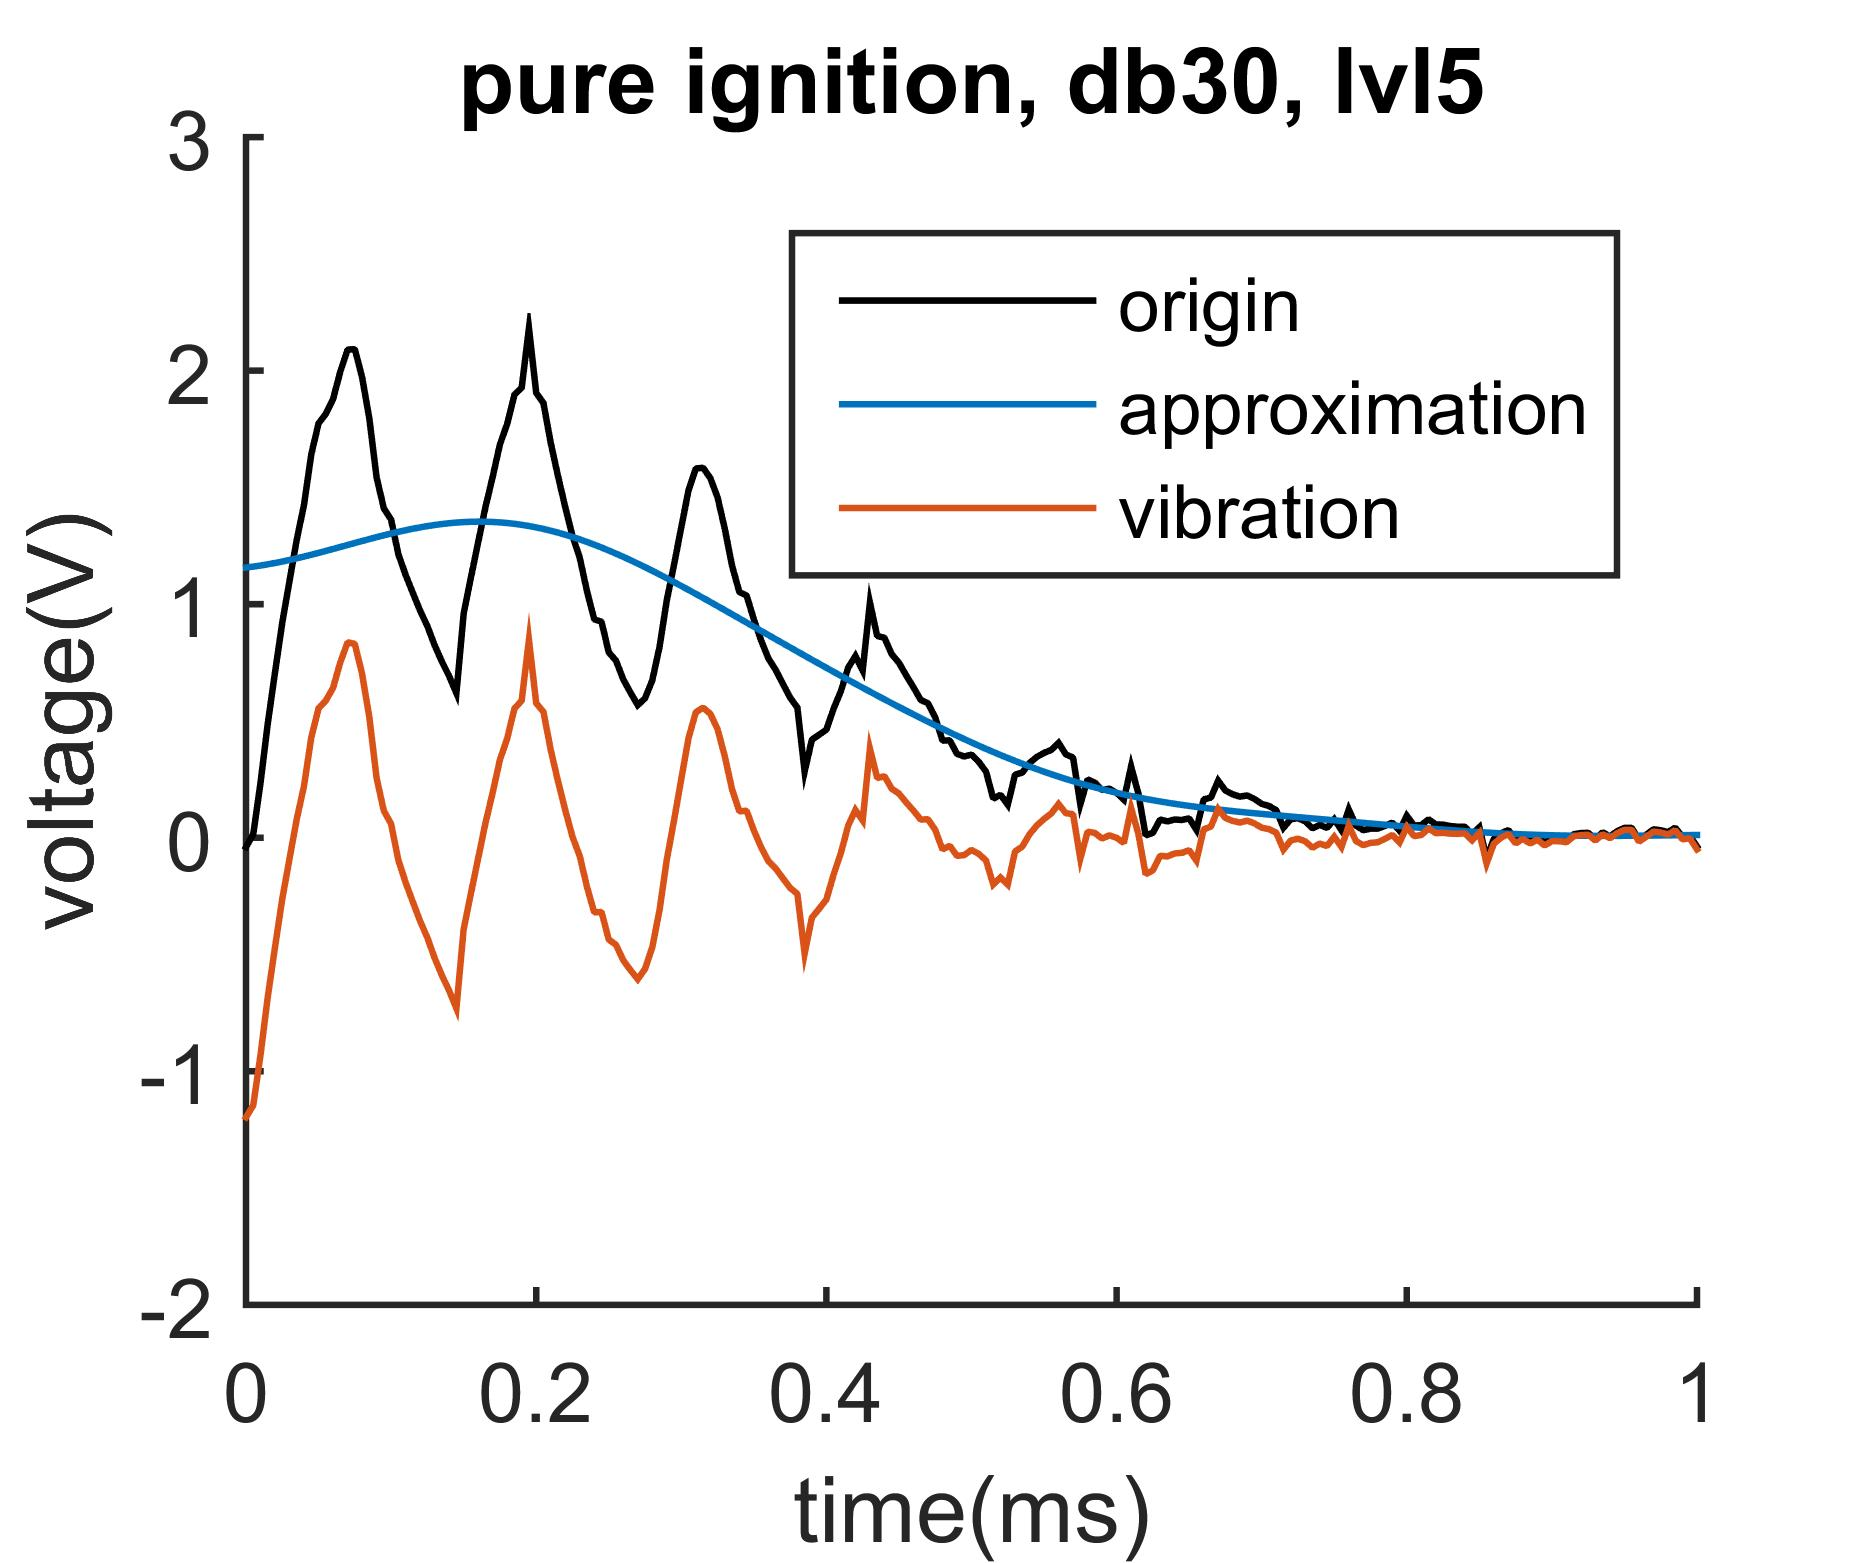
\includegraphics[width=0.3\textwidth]{thesis_figure/ion_chapter/db30_lvl5}
	\end{tabular}
	\caption{\label{fig:dbvar}不同阶数下的db小波第五层分解}
\end{figure}
从图\ref{fig:dbvar}中可以看到当阶数增加后,小波第五层分解的结果不变,考虑到分解阶数越多计算越加复杂。则取db20作为db小波分解的小波函数。
\subsection{sym小波族的阶数选择和分析}
\begin{figure}[H]
	\centering
	\begin{tabular}{ccc}
		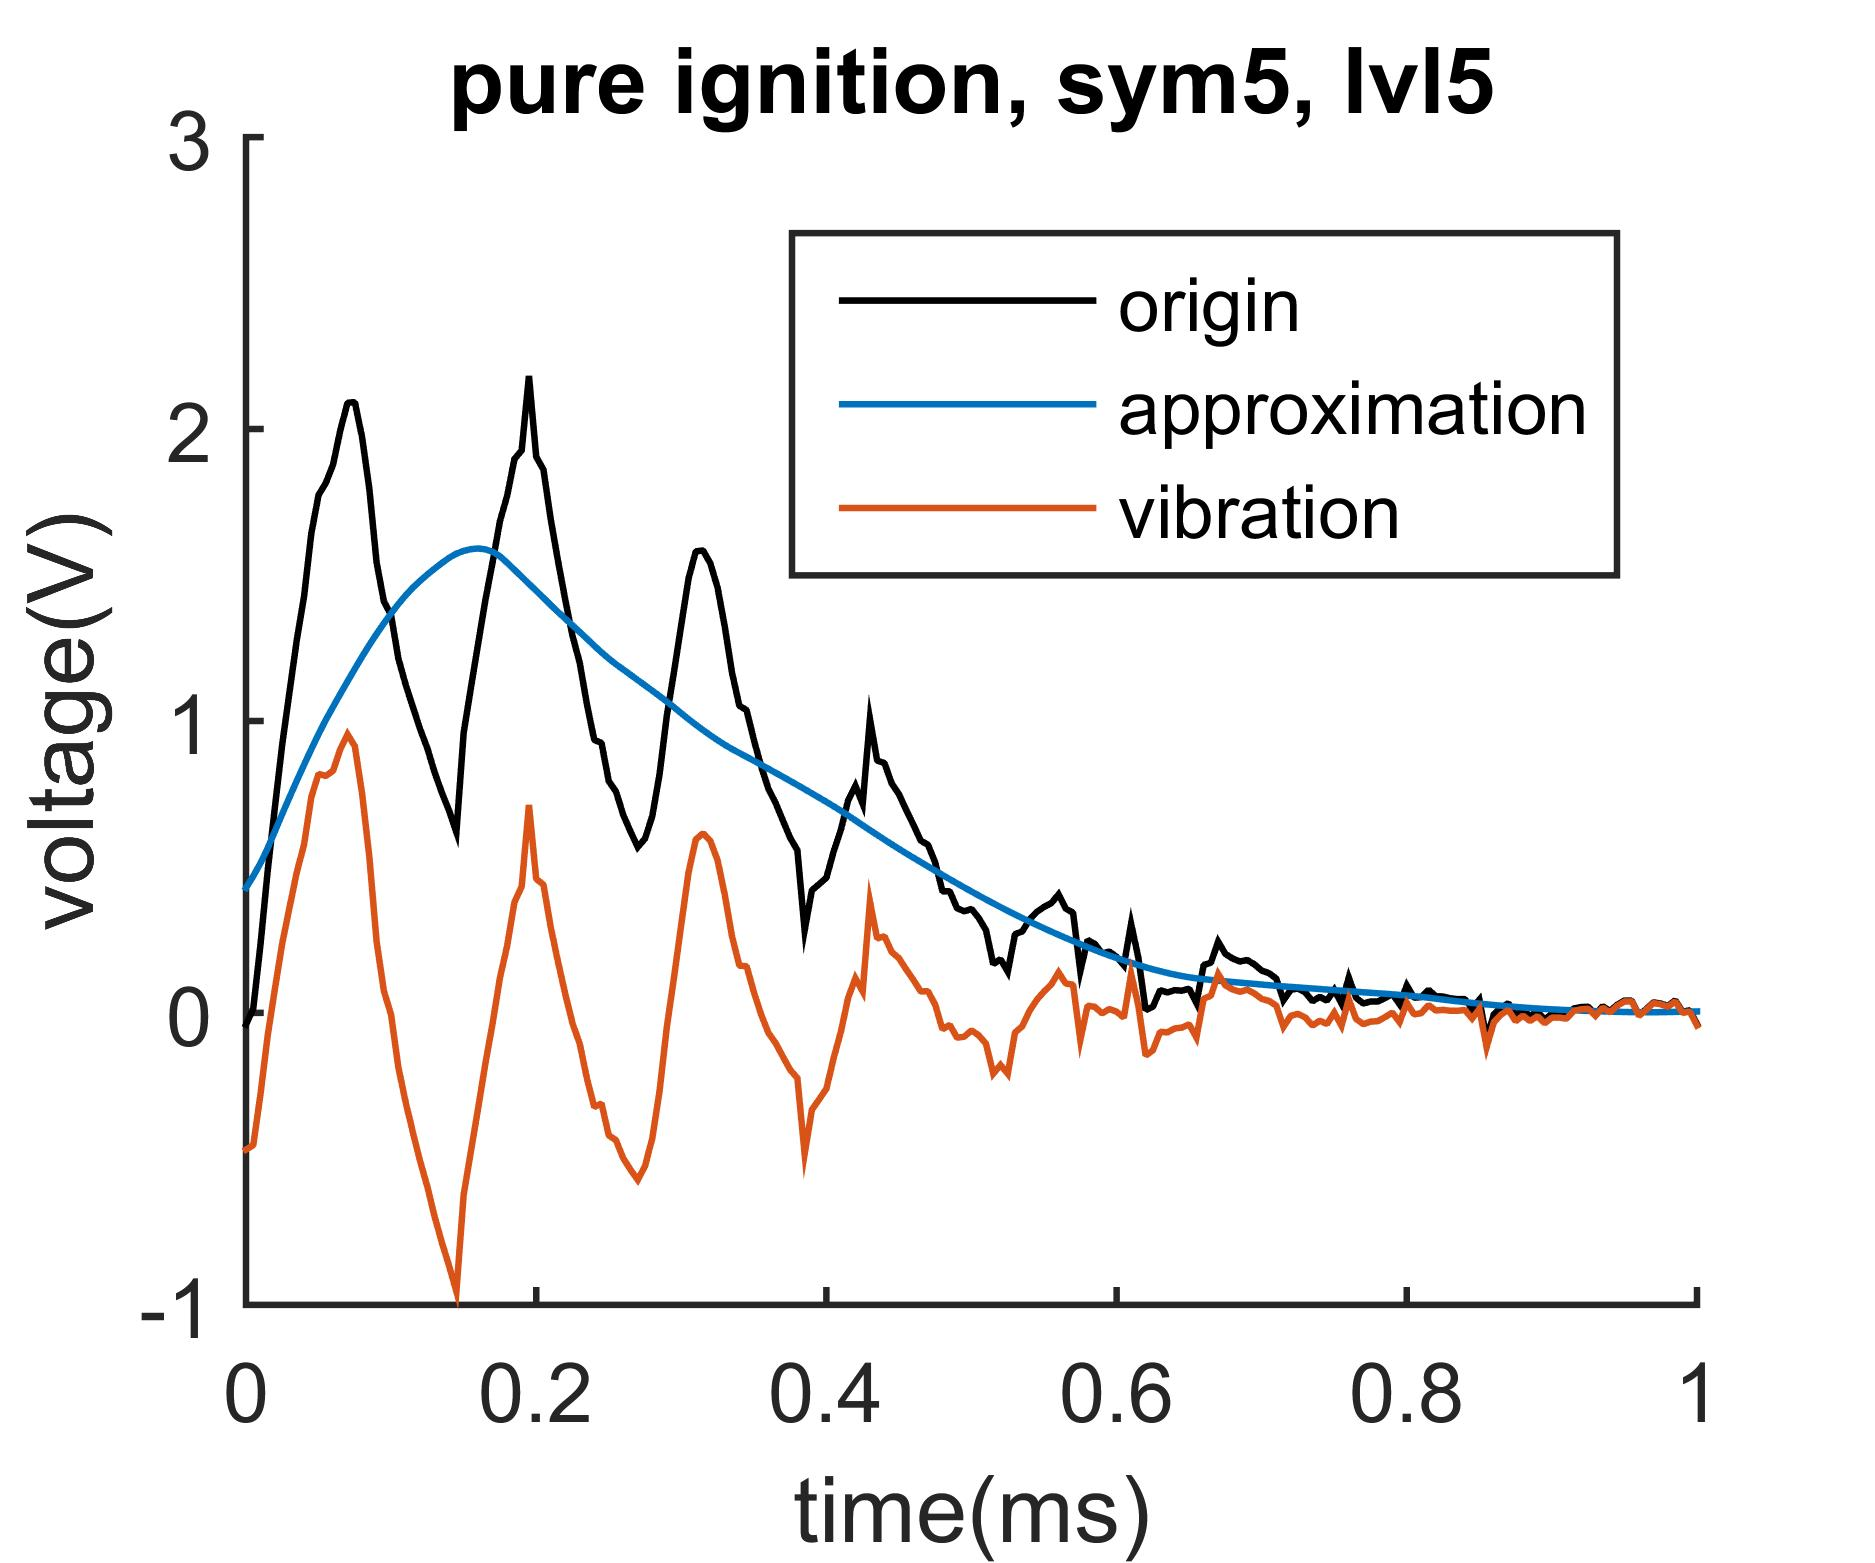
\includegraphics[width=0.3\textwidth]{thesis_figure/ion_chapter/sym5_lvl5}&
		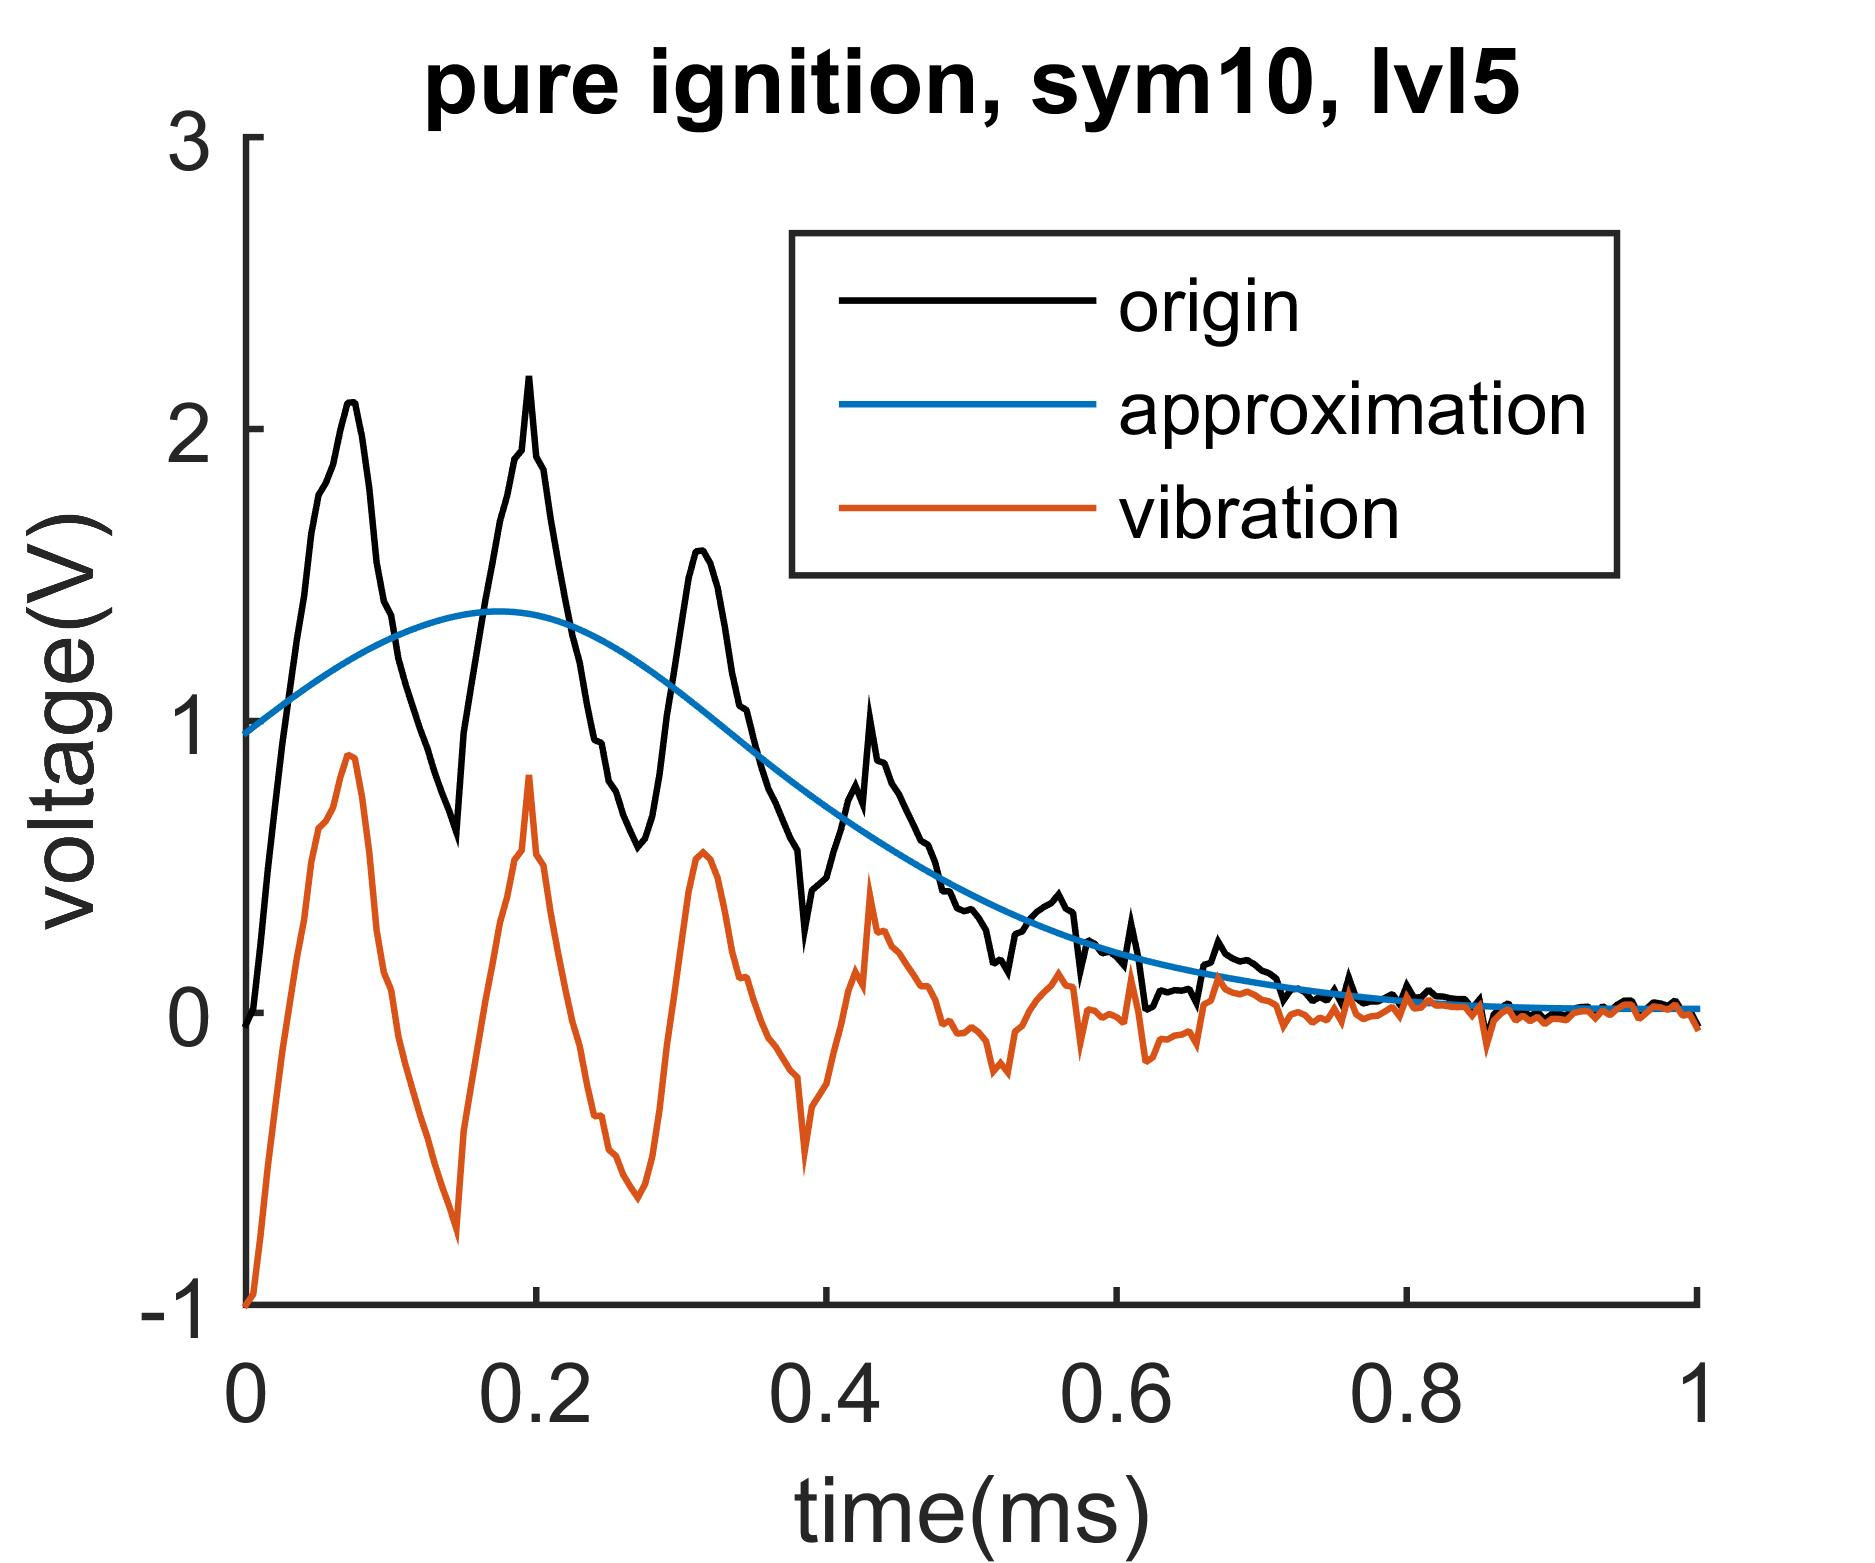
\includegraphics[width=0.3\textwidth]{thesis_figure/ion_chapter/sym10_lvl5}&
		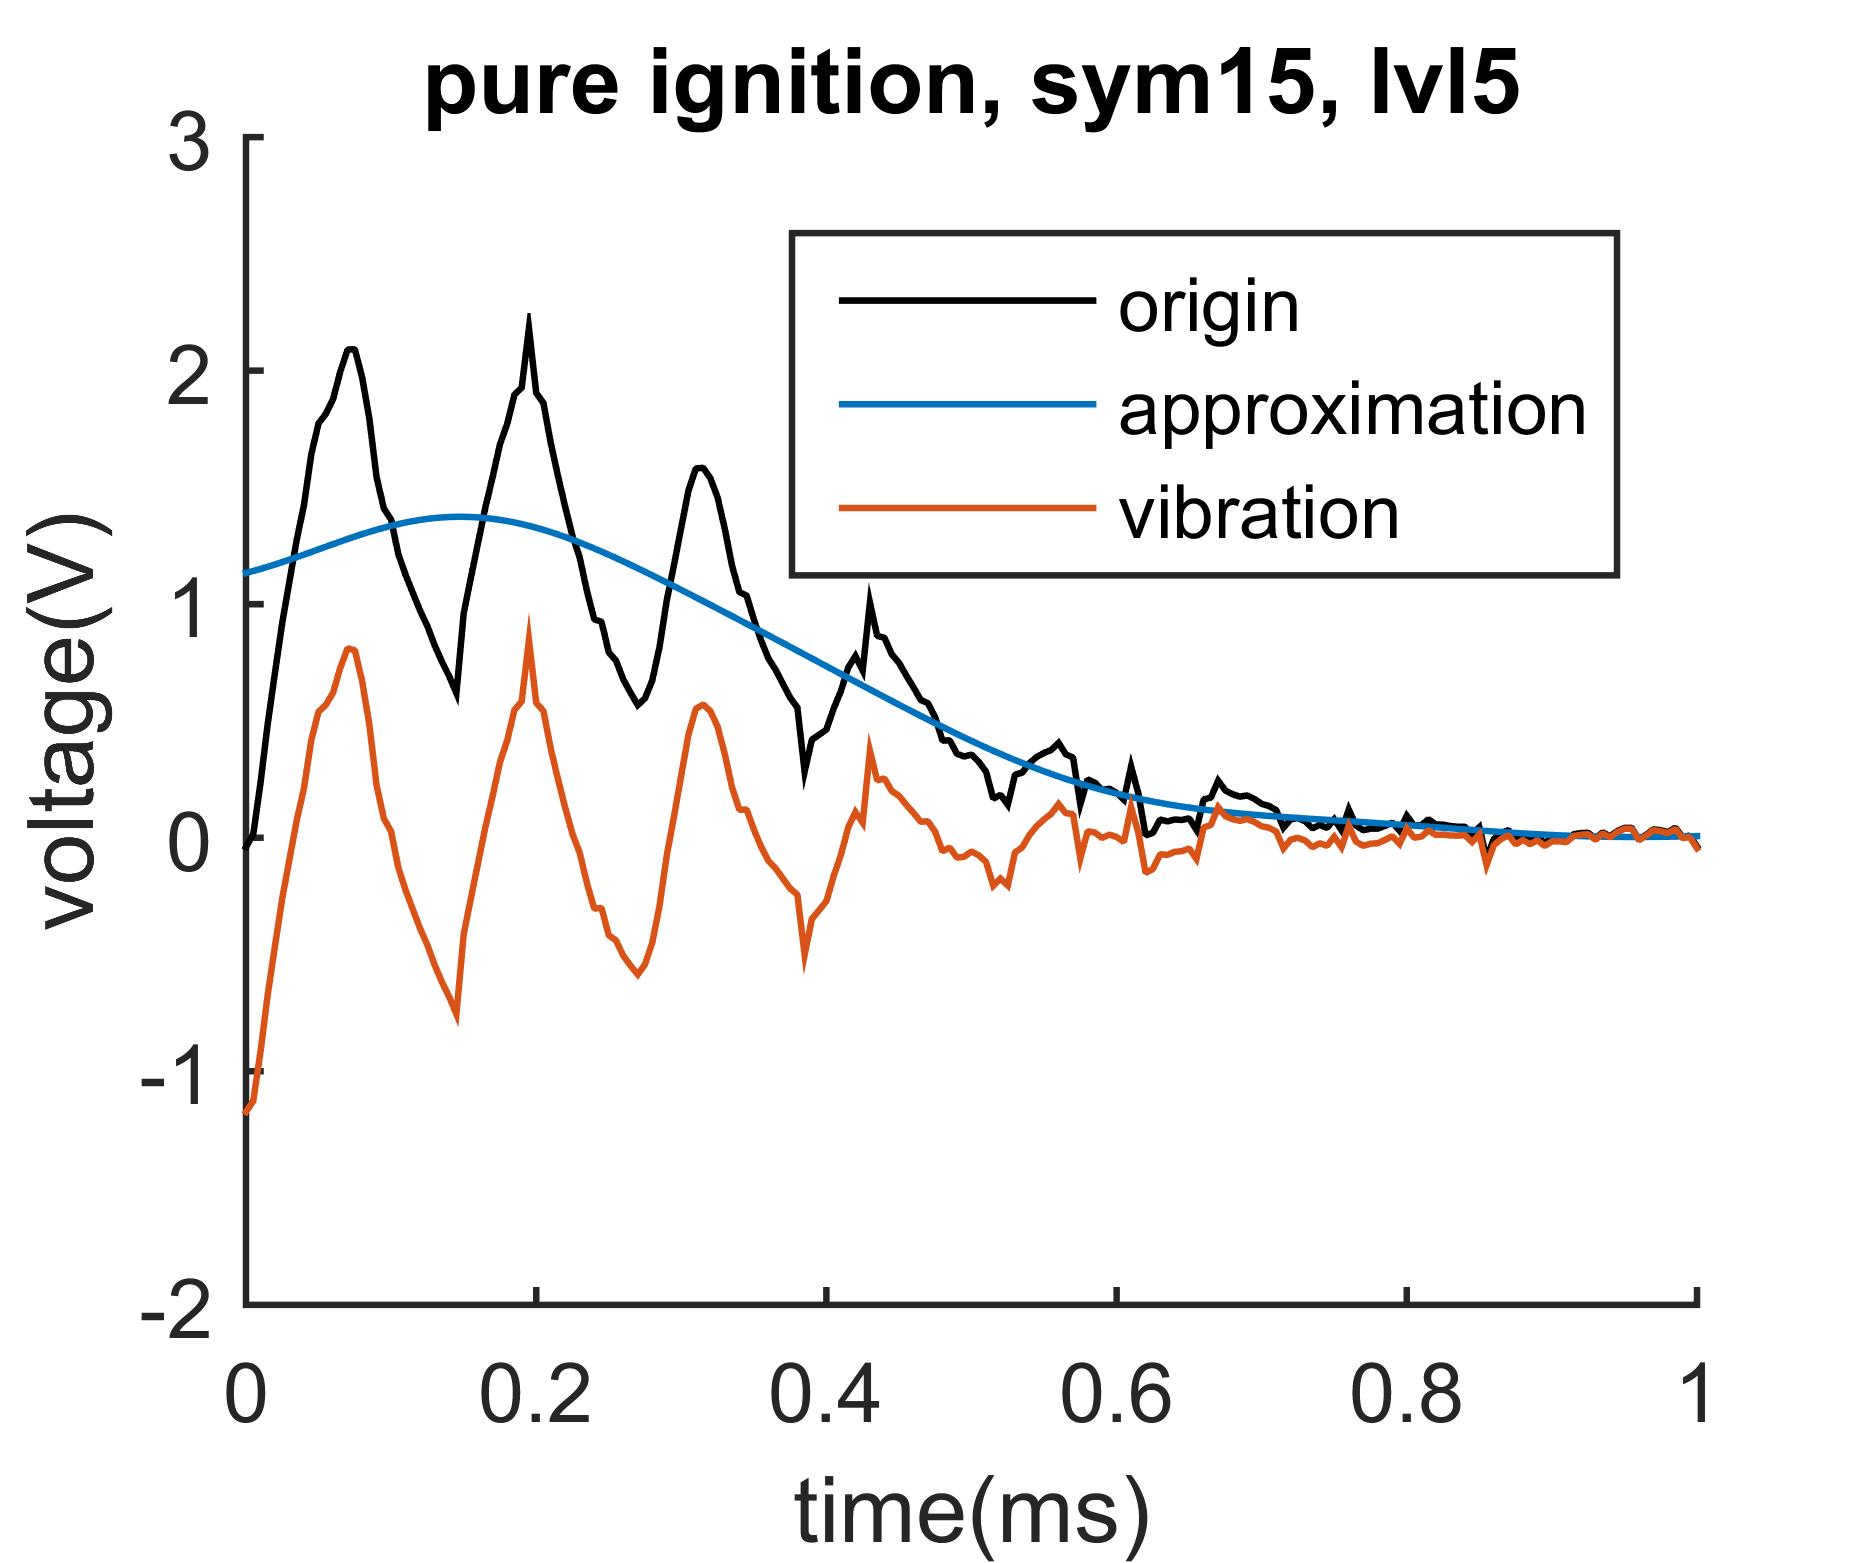
\includegraphics[width=0.3\textwidth]{thesis_figure/ion_chapter/sym15_lvl5}\\
		\includegraphics[width=0.3\textwidth]{thesis_figure/ion_chapter/sym20_lvl5}&
		\includegraphics[width=0.3\textwidth]{thesis_figure/ion_chapter/sym25_lvl5}&
		\includegraphics[width=0.3\textwidth]{thesis_figure/ion_chapter/sym30_lvl5}
	\end{tabular}
	\caption{\label{fig:symvar}不同阶数下的sym小波第五层分解}
\end{figure}
从图\ref{fig:symvar}中可以看到当阶数增加到20以后,小波分析第五层分解的结果已经基本不变了,而且随着阶数的增加,sym小波分解的时间增加很快。则取sym20作为sym小波分解的小波函数。
\subsection{四种小波对去除点火干扰分析的比较}
去除点火干扰的方法为用同一个小波基函数对离子电流信号和纯点火干扰信号进行分析,然后两者做差值得出理想的离子电流信号。
\begin{figure}[!ht]
	\centering
	\begin{tabular}{ccc}
		\includegraphics[width=0.4\textwidth]{thesis_figure/ion_chapter/dmey_wafig_pureign}&
		\includegraphics[width=0.4\textwidth]{thesis_figure/ion_chapter/dmey_icfig_norm}\\
		\includegraphics[width=0.4\textwidth]{thesis_figure/ion_chapter/dmey_diffSign}&
		\includegraphics[width=0.4\textwidth]{thesis_figure/ion_chapter/dmey_realIonFig}
	\end{tabular}
	\caption{\label{fig:dmey_realIon}dmey小波分解的真实离子电流信号}
\end{figure}
\par如图\ref{fig:dmey_realIon}所示的用dmey小波基函数进行小波分析得到的纯点火干扰、离子电流的分解、真实离子电流以及原信号和提取信号比较图。此时的工况为$1000r/min$、40\%负荷,在
此工况下热电离产生的波峰不会被点火干扰淹没。从图中可以看到提取信号可以很好的和原离子电流的其他信号部分进行衔接。从左下角的差值信号中可以看到,该信号存在一个凸起的小峰,此峰即是火焰前锋期造成的离子电流峰,
是火焰锋面从电极一端向另一端扩散过程中化学电离产生的离子电流。
\begin{figure}[!ht]
	\centering
	\includegraphics[width=0.5\textwidth]{thesis_figure/ion_chapter/diff_wv_comp}
	\caption{\label{fig:diff_wv_comp}四种小波对真实离子电流进行去干扰处理}
\end{figure}
\par下图\ref{fig:diff_wv_comp}所示是四种小波对真实离子电流进行处理后的信号比较。从图中可以看到曲线的尖锐程度依次为$dmey>coif>db>sym$,但是差异不大,
都能够明显的显示出火焰前锋期的形状。\par从相位角度来衡量,四种小波基函数分析结果在关键点的相位上是一样的,能够确定火焰前锋期的开始和结束相位。在曲线的尾段有不同的曲线效果,
这是不同的小波基函数分析结果的最大不同。
\section{高斯曲线拟合估计离子电流特征参数}
\subsection{高斯曲线拟合方法介绍}
来自马里兰大学的T. C. O'Haver给出了曲线拟合的方法\cite{tco_gs}能够有效的对数据进行拟合。根据拟合公式\ref{eqn:interp1}和\ref{eqn:interp2}可以知道,我们可以用两个高斯
函数来对小波分析处理后的离子电流信号曲线进行拟合,从而得到离子电流的关键特征参数。采集到的离子电流曲线有很多杂乱信号,而且整个信号也有部分波动,有较多的峰值。只有通过函数拟合的方
式,才能够较好的获得离子电流特征参数。
\par拟合方法优劣的评判标准主要是误差分析。
\subsection{双高斯曲线拟合}
给定在$1000r/min$、40\%负荷时的经过小波分析去除干扰的离子电流,经过双高斯曲线拟合方法得到如图所示的曲线。
\chapter{离子电流工况拓展的预测与验证}
\section{离子电流淹没情况下对缸压的预测}

\section{离子电流淹没情况下对空燃比的预测}
\chapter{总结及展望}
\section{全文总结}
\section{工作展望}

%%% 其它部分
\backmatter

\makeatother

% 参考文献
\bibliographystyle{tongjibib}
\bibliography{ref/ref_thesis}

% 致谢
% !TeX encoding = GB2312

%%% Local Variables:
%%% mode: latex
%%% TeX-master: "../main"
%%% End:

\begin{ack}
  ���ĸ�л��ʦ��־�����ڶԱ��˵ľ���ָ�������ǵ��Դ����̽�ʹ
  ���������档

  ��������ʡ����ѧԺ��ѧϵ���оŸ��µĺ����о��ڼ䣬���� xxx ��������ָ�����������
  ʤ�м�����л xx ʵ�������� xx ���ڣ��Լ�ʵ����ȫ����ʦ��ͬѧ�ǵ����������֧
  �֣���������ɹ�����Ȼ��ѧ�����������ش���л��

  ��л \tongjithesis{}�����Ĵ������ҵ�����д���������������࣬���ҵ����ĸ�ʽ����Ư����
  ���ࡣ

\end{ack}


% 附录
%\begin{appendix}
%%%% Local Variables:
%%% mode: latex
%%% TeX-master: "../main"
%%% End:

\chapter{外文资料原文}
\label{cha:engorg}
As one of the most widely used techniques in operations research, {\em
  mathematical programming} is defined as a means of maximizing a quantity known
as {\em objective function}, subject to a set of constraints represented by
equations and inequalities. Some known subtopics of mathematical programming are
linear programming, nonlinear programming, multiobjective programming, goal
programming, dynamic programming, and multilevel programming$^{[1]}$.

It is impossible to cover in a single chapter every concept of mathematical
programming. This chapter introduces only the basic concepts and techniques of
mathematical programming such that readers gain an understanding of them
throughout the book$^{[2,3]}$.


\section{Single-Objective Programming}
The general form of single-objective programming (SOP) is written
as follows,
\begin{equation}\tag*{(123)} % 如果附录中的公式不想让它出现在公式索引中,那就请
                             % 用 \tag*{xxxx}
\left\{\begin{array}{l}
\max \,\,f(x)\\[0.1 cm]
\mbox{subject to:} \\ [0.1 cm]
\qquad g_j(x)\le 0,\quad j=1,2,\cdots,p
\end{array}\right.
\end{equation}
which maximizes a real-valued function $f$ of
$x=(x_1,x_2,\cdots,x_n)$ subject to a set of constraints.

\newtheorem{mpdef}{Definition}[chapter]
\begin{mpdef}
In SOP, we call $x$ a decision vector, and
$x_1,x_2,\cdots,x_n$ decision variables. The function
$f$ is called the objective function. The set
\begin{equation}\tag*{(456)} % 这里同理,其它不再一一指定。
S=\left\{x\in\Re^n\bigm|g_j(x)\le 0,\,j=1,2,\cdots,p\right\}
\end{equation}
is called the feasible set. An element $x$ in $S$ is called a
feasible solution.
\end{mpdef}

\newtheorem{mpdefop}[mpdef]{Definition}
\begin{mpdefop}
A feasible solution $x^*$ is called the optimal
solution of SOP if and only if
\begin{equation}
f(x^*)\ge f(x)
\end{equation}
for any feasible solution $x$.
\end{mpdefop}

One of the outstanding contributions to mathematical programming was known as
the Kuhn-Tucker conditions\ref{eq:ktc}. In order to introduce them, let us give
some definitions. An inequality constraint $g_j(x)\le 0$ is said to be active at
a point $x^*$ if $g_j(x^*)=0$. A point $x^*$ satisfying $g_j(x^*)\le 0$ is said
to be regular if the gradient vectors $\nabla g_j(x)$ of all active constraints
are linearly independent.

Let $x^*$ be a regular point of the constraints of SOP and assume that all the
functions $f(x)$ and $g_j(x),j=1,2,\cdots,p$ are differentiable. If $x^*$ is a
local optimal solution, then there exist Lagrange multipliers
$\lambda_j,j=1,2,\cdots,p$ such that the following Kuhn-Tucker conditions hold,
\begin{equation}
\label{eq:ktc}
\left\{\begin{array}{l}
    \nabla f(x^*)-\sum\limits_{j=1}^p\lambda_j\nabla g_j(x^*)=0\\[0.3cm]
    \lambda_jg_j(x^*)=0,\quad j=1,2,\cdots,p\\[0.2cm]
    \lambda_j\ge 0,\quad j=1,2,\cdots,p.
\end{array}\right.
\end{equation}
If all the functions $f(x)$ and $g_j(x),j=1,2,\cdots,p$ are convex and
differentiable, and the point $x^*$ satisfies the Kuhn-Tucker conditions
(\ref{eq:ktc}), then it has been proved that the point $x^*$ is a global optimal
solution of SOP.

\subsection{Linear Programming}
\label{sec:lp}

If the functions $f(x),g_j(x),j=1,2,\cdots,p$ are all linear, then SOP is called
a {\em linear programming}.

The feasible set of linear is always convex. A point $x$ is called an extreme
point of convex set $S$ if $x\in S$ and $x$ cannot be expressed as a convex
combination of two points in $S$. It has been shown that the optimal solution to
linear programming corresponds to an extreme point of its feasible set provided
that the feasible set $S$ is bounded. This fact is the basis of the {\em simplex
  algorithm} which was developed by Dantzig as a very efficient method for
solving linear programming.
\begin{table}[ht]
\centering
  \centering
  \caption*{Table~1\hskip1em This is an example for manually numbered table, which
    would not appear in the list of tables}
  \label{tab:badtabular2}
  \begin{tabular}[c]{|c|m{0.8in}|c|c|c|c|c|}\hline
    \multicolumn{2}{|c|}{Network Topology} & \# of nodes &
    \multicolumn{3}{c|}{\# of clients} & Server \\\hline
    GT-ITM & Waxman Transit-Stub & 600 &
    \multirow{2}{2em}{2\%}&
    \multirow{2}{2em}{10\%}&
    \multirow{2}{2em}{50\%}&
    \multirow{2}{1.2in}{Max. Connectivity}\\\cline{1-3}
    \multicolumn{2}{|c|}{Inet-2.1} & 6000 & & & &\\\hline
    \multirow{2}{1in}{Xue} & Rui  & Ni &\multicolumn{4}{c|}{\multirow{2}*{\tongjithesis}}\\\cline{2-3}
    & \multicolumn{2}{c|}{ABCDEF} &\multicolumn{4}{c|}{} \\\hline
\end{tabular}
\end{table}

Roughly speaking, the simplex algorithm examines only the extreme points of the
feasible set, rather than all feasible points. At first, the simplex algorithm
selects an extreme point as the initial point. The successive extreme point is
selected so as to improve the objective function value. The procedure is
repeated until no improvement in objective function value can be made. The last
extreme point is the optimal solution.

\subsection{Nonlinear Programming}

If at least one of the functions $f(x),g_j(x),j=1,2,\cdots,p$ is nonlinear, then
SOP is called a {\em nonlinear programming}.

A large number of classical optimization methods have been developed to treat
special-structural nonlinear programming based on the mathematical theory
concerned with analyzing the structure of problems.
\begin{figure}[h]
  \centering
  \includegraphics[clip]{tongji-lib-logo.jpg}
  \caption*{Figure~1\hskip1em This is an example for manually numbered figure,
    which would not appear in the list of figures}
  \label{tab:badfigure2}
\end{figure}

Now we consider a nonlinear programming which is confronted solely with
maximizing a real-valued function with domain $\Re^n$.  Whether derivatives are
available or not, the usual strategy is first to select a point in $\Re^n$ which
is thought to be the most likely place where the maximum exists. If there is no
information available on which to base such a selection, a point is chosen at
random. From this first point an attempt is made to construct a sequence of
points, each of which yields an improved objective function value over its
predecessor. The next point to be added to the sequence is chosen by analyzing
the behavior of the function at the previous points. This construction continues
until some termination criterion is met. Methods based upon this strategy are
called {\em ascent methods}, which can be classified as {\em direct methods},
{\em gradient methods}, and {\em Hessian methods} according to the information
about the behavior of objective function $f$. Direct methods require only that
the function can be evaluated at each point. Gradient methods require the
evaluation of first derivatives of $f$. Hessian methods require the evaluation
of second derivatives. In fact, there is no superior method for all
problems. The efficiency of a method is very much dependent upon the objective
function.

\subsection{Integer Programming}

{\em Integer programming} is a special mathematical programming in which all of
the variables are assumed to be only integer values. When there are not only
integer variables but also conventional continuous variables, we call it {\em
  mixed integer programming}. If all the variables are assumed either 0 or 1,
then the problem is termed a {\em zero-one programming}. Although integer
programming can be solved by an {\em exhaustive enumeration} theoretically, it
is impractical to solve realistically sized integer programming problems. The
most successful algorithm so far found to solve integer programming is called
the {\em branch-and-bound enumeration} developed by Balas (1965) and Dakin
(1965). The other technique to integer programming is the {\em cutting plane
  method} developed by Gomory (1959).

\hfill\textit{Uncertain Programming\/}\quad(\textsl{BaoDing Liu, 2006.2})

\section*{References}
\noindent{\itshape NOTE: these references are only for demonstration, they are
  not real citations in the original text.}

\begin{enumerate}[{$[$}1{$]$}]
\item Donald E. Knuth. The \TeX book. Addison-Wesley, 1984. ISBN: 0-201-13448-9
\item Paul W. Abrahams, Karl Berry and Kathryn A. Hargreaves. \TeX\ for the
  Impatient. Addison-Wesley, 1990. ISBN: 0-201-51375-7
\item David Salomon. The advanced \TeX book.  New York : Springer, 1995. ISBN:0-387-94556-3
\end{enumerate}

\chapter{外文资料的调研阅读报告或书面翻译}
\section{单目标规划}
北冥有鱼,其名为鲲。鲲之大,不知其几千里也。化而为鸟,其名为鹏。鹏之背,不知其几
千里也。怒而飞,其翼若垂天之云。是鸟也,海运则将徙于南冥。南冥者,天池也。
\begin{equation}\tag*{(123)}
 p(y|\mathbf{x}) = \frac{p(\mathbf{x},y)}{p(\mathbf{x})}=
\frac{p(\mathbf{x}|y)p(y)}{p(\mathbf{x})}
\end{equation}

吾生也有涯,而知也无涯。以有涯随无涯,殆已!已而为知者,殆而已矣!为善无近名,为
恶无近刑,缘督以为经,可以保身,可以全生,可以养亲,可以尽年。

\subsection{线性规划}
庖丁为文惠君解牛,手之所触,肩之所倚,足之所履,膝之所倚,砉然响然,奏刀騞然,莫
不中音,合于桑林之舞,乃中经首之会。
\begin{table}[ht]
\centering
  \centering
  \caption*{表~1\hskip1em 这是手动编号但不出现在索引中的一个表格例子}
  \label{tab:badtabular3}
  \begin{tabular}[c]{|c|m{0.8in}|c|c|c|c|c|}\hline
    \multicolumn{2}{|c|}{Network Topology} & \# of nodes &
    \multicolumn{3}{c|}{\# of clients} & Server \\\hline
    GT-ITM & Waxman Transit-Stub & 600 &
    \multirow{2}{2em}{2\%}&
    \multirow{2}{2em}{10\%}&
    \multirow{2}{2em}{50\%}&
    \multirow{2}{1.2in}{Max. Connectivity}\\\cline{1-3}
    \multicolumn{2}{|c|}{Inet-2.1} & 6000 & & & &\\\hline
    \multirow{2}{1in}{Xue} & Rui  & Ni &\multicolumn{4}{c|}{\multirow{2}*{\tongjithesis}}\\\cline{2-3}
    & \multicolumn{2}{c|}{ABCDEF} &\multicolumn{4}{c|}{} \\\hline
\end{tabular}
\end{table}

文惠君曰:“嘻,善哉!技盖至此乎?”庖丁释刀对曰:“臣之所好者道也,进乎技矣。始臣之
解牛之时,所见无非全牛者;三年之后,未尝见全牛也;方今之时,臣以神遇而不以目视,
官知止而神欲行。依乎天理,批大郤,导大窾,因其固然。技经肯綮之未尝,而况大坬乎!
良庖岁更刀,割也;族庖月更刀,折也;今臣之刀十九年矣,所解数千牛矣,而刀刃若新发
于硎。彼节者有间而刀刃者无厚,以无厚入有间,恢恢乎其于游刃必有余地矣。是以十九年
而刀刃若新发于硎。虽然,每至于族,吾见其难为,怵然为戒,视为止,行为迟,动刀甚微,
謋然已解,如土委地。提刀而立,为之而四顾,为之踌躇满志,善刀而藏之。”

文惠君曰:“善哉!吾闻庖丁之言,得养生焉。”


\subsection{非线性规划}
孔子与柳下季为友,柳下季之弟名曰盗跖。盗跖从卒九千人,横行天下,侵暴诸侯。穴室枢
户,驱人牛马,取人妇女。贪得忘亲,不顾父母兄弟,不祭先祖。所过之邑,大国守城,小
国入保,万民苦之。孔子谓柳下季曰:“夫为人父者,必能诏其子;为人兄者,必能教其弟。
若父不能诏其子,兄不能教其弟,则无贵父子兄弟之亲矣。今先生,世之才士也,弟为盗
跖,为天下害,而弗能教也,丘窃为先生羞之。丘请为先生往说之。”
\begin{figure}[h]
  \centering
  \includegraphics{hello}
  \caption*{图~1\hskip1em 这是手动编号但不出现索引中的图片的例子}
  \label{tab:badfigure3}
\end{figure}

柳下季曰:“先生言为人父者必能诏其子,为人兄者必能教其弟,若子不听父之诏,弟不受
兄之教,虽今先生之辩,将奈之何哉?且跖之为人也,心如涌泉,意如飘风,强足以距敌,
辩足以饰非。顺其心则喜,逆其心则怒,易辱人以言。先生必无往。”

孔子不听,颜回为驭,子贡为右,往见盗跖。

\subsection{整数规划}
盗跖乃方休卒徒大山之阳,脍人肝而餔之。孔子下车而前,见谒者曰:“鲁人孔丘,闻将军
高义,敬再拜谒者。”谒者入通。盗跖闻之大怒,目如明星,发上指冠,曰:“此夫鲁国之
巧伪人孔丘非邪?为我告之:尔作言造语,妄称文、武,冠枝木之冠,带死牛之胁,多辞缪
说,不耕而食,不织而衣,摇唇鼓舌,擅生是非,以迷天下之主,使天下学士不反其本,妄
作孝弟,而侥幸于封侯富贵者也。子之罪大极重,疾走归!不然,我将以子肝益昼餔之膳。”


\chapter{其它附录}
其它附录的内容可以放到这里,当然如果你愿意,可以把这部分也放到独立的文件中,然后
将其\verb|\input| 到主文件中。

%\end{appendix}

% 个人简历
% !TeX encoding = GB2312
\begin{resume}

  \resumeitem{���˼���}

  xxxx �� xx �� xx �ճ����� xx ʡ xx �ء�
  
  xxxx �� 9 �¿��� xx ��ѧ xx ϵ xx רҵ��xxxx �� 7 �±��Ʊ�ҵ����� xx ѧʿѧλ��
  
  xxxx �� 9 �����Խ��� xx ��ѧ xx ϵ���� xx ѧλ����

  \resumeitem{������ѧ������} % �����ĺ�¼�õĺ���һ��

  \begin{enumerate}[{[}1{]}]
  \item Yang Y, Ren T L, Zhang L T, et al. Miniature microphone with silicon-
    based ferroelectric thin films. Integrated Ferroelectrics, 2003,
    52:229-235. (SCI ��¼, ������:758FZ.)
  \item ����, ������, ������, ��. �������΢��ѧ�����б�Ĥ����Ӧ�����о�. �й���
    е����, 2005, 16(14):1289-1291. (EI ��¼, ������:0534931 2907.)
  \item ����, ������, ������, ��. �������������еĹؼ������о�. �����DZ�ѧ��,
    2003, 24(S4):192-193. (EI Դ��.)
  \item Yang Y, Ren T L, Zhu Y P, et al. PMUTs for handwriting recognition. In
    press. (�ѱ� Integrated Ferroelectrics ¼��. SCI Դ��.)
  \item Wu X M, Yang Y, Cai J, et al. Measurements of ferroelectric MEMS
    microphones. Integrated Ferroelectrics, 2005, 69:417-429. (SCI ��¼, ������
    :896KM.)
  \item ����, ����, �¾�, ��. ����ѹ��͵���΢��˷����踯ʴ����о�. ѹ������
    ��, 2006, 28(1):117-119. (EI ��¼, ������:06129773469.)
  \item ������, ����, ������, ��. ����MEMS�����ļ��������΢��˷�. �й����ɵ�·, 
    2003, 53:59-61.
  \end{enumerate}

  \resumeitem{�о��ɹ�} % �о�д��û�о�ɾ��
  \begin{enumerate}[{[}1{]}]
  \item ������, ����, ��һƽ, ��. �������΢��ѧ�������뼫��������ƺ͵缫���ӵ�
    ����: �й�, CN1602118A. (�й�ר��������.)
  \item Ren T L, Yang Y, Zhu Y P, et al. Piezoelectric micro acoustic sensor
    based on ferroelectric materials: USA, No.11/215, 102. (��������ר�������.)
  \end{enumerate}
\end{resume}

\end{document}
